\documentclass{article}
%%================================
% note-setup-leftbar.tex
% fenglielie@qq.com 2026-08-21
%================================

\usepackage{amsmath,amsthm,amssymb}
\usepackage{mathtools}
\usepackage{mathrsfs}
\usepackage{bm}
\usepackage{extarrows}
\usepackage[a4paper, margin=1cm, footskip=0.5cm]{geometry}
\usepackage{float}
\usepackage{indentfirst}
\usepackage{booktabs,multirow}
\usepackage[shortlabels,inline]{enumitem}
\usepackage{appendix}

%%================================
%% FIX GLOBALE PER LISTE DOPO I TEOREMI
%%================================
% Risolve il "primo punto a destra del titolo" quando itemize/enumerate 
% seguono immediatamente l'apertura di un ambiente theorem-like.
\makeatletter
\AddToHook{env/itemize/begin}{\if@inlabel\mbox{}\par\vspace{-\baselineskip}\fi}
\AddToHook{env/enumerate/begin}{\if@inlabel\mbox{}\par\vspace{-\baselineskip}\fi}
\makeatother
%%================================

\usepackage[dvipsnames]{xcolor}
\usepackage{pifont}
\usepackage{graphicx}
\graphicspath{
    {./figure/}{./figures/}{./image/}{./images/}{./graphic/}{./graphics/}{./picture/}{./pictures/}
}
\usepackage{subcaption}

\usepackage[ruled,linesnumbered,noline]{algorithm2e}
\usepackage{listings}
\lstdefinestyle{simpleStyle}{
    basicstyle=\ttfamily\small,
    breaklines=true,
    keywordstyle=\color{blue},
    identifierstyle=\color{black},
    stringstyle=\color{violet},
    commentstyle=\color[RGB]{34,139,34},
    showstringspaces=false,
    numbers=left,
    numbersep=2em,
    numberstyle=\footnotesize,
    frame=single,
    framesep=1em,
}
\lstset{style=simpleStyle}

\usepackage{hyperref}
\hypersetup{
    colorlinks=true,linkcolor=,urlcolor=cyan
}

\usepackage[most]{tcolorbox}
\usepackage{keytheorems}

\tcbset{
    theorem box/.style={
            enhanced,
            breakable,
            sharp corners,
            leftrule=2pt,
            rightrule=0pt,
            toprule=0pt,
            bottomrule=0pt,
        },
    theorem box rounded/.style={
            theorem box,
            rounded corners,
        }
}

%%================================
%% STILI UFFICIALI KEYTHEOREMS
%%================================
\newkeytheoremstyle{breakplain}{
    inherit-style=plain,
    headpunct={},
    break
}
\newkeytheoremstyle{breakdefinition}{
    inherit-style=definition,
    headpunct={},
    break
}
\newkeytheoremstyle{breakremark}{
    inherit-style=remark,
    headpunct={},
    break
}
\newkeytheoremstyle{notestyle}{
    headfont=\color{orange!80!black}\bfseries,
    bodyfont=\normalfont,
    spaceabove=3pt,
    spacebelow=3pt,
    headpunct={},
    break,
    qed=\ensuremath{\color{orange!80!black}\diamond}
}
\newkeytheoremstyle{solutionstyle}{
    headfont=\bfseries,
    bodyfont=\normalfont,
    spaceabove=3pt,
    spacebelow=3pt,
    headpunct={},
    break,
    qed=\ensuremath{\square}
}

%%================================
%% DEFINIZIONE AMBIENTI
%%================================

\newkeytheorem{theorem}[style=breakplain, name=Teorema, numbered=true, parent=section,
    tcolorbox-no-titlebar={theorem box, colframe=RoyalPurple, colback=RoyalPurple!8}]
\newkeytheorem{theorem*}[style=breakplain, name=Teorema, numbered=false,
    tcolorbox-no-titlebar={theorem box rounded, colframe=RoyalPurple, colback=RoyalPurple!8}]

\newkeytheorem{prop}[style=breakplain, name=Proposizione, numbered=true, sibling=theorem,
    tcolorbox-no-titlebar={theorem box, colframe=RoyalPurple, colback=RoyalPurple!8}]
\newkeytheorem{prop*}[style=breakplain, name=Proposizione, numbered=false,
    tcolorbox-no-titlebar={theorem box rounded, colframe=RoyalPurple, colback=RoyalPurple!8}]

\newkeytheorem{corollary}[style=breakplain, name=Corollario, numbered=true, sibling=theorem,
    tcolorbox-no-titlebar={theorem box, colframe=NavyBlue, colback=SkyBlue!8}]
\newkeytheorem{corollary*}[style=breakplain, name=Corollario, numbered=false,
    tcolorbox-no-titlebar={theorem box rounded, colframe=NavyBlue, colback=SkyBlue!8}]

\newkeytheorem{lemma}[style=breakplain, name=Lemma, numbered=true, sibling=theorem,
    tcolorbox-no-titlebar={theorem box, colframe=NavyBlue, colback=SkyBlue!8}]
\newkeytheorem{lemma*}[style=breakplain, name=Lemma, numbered=false,
    tcolorbox-no-titlebar={theorem box rounded, colframe=NavyBlue, colback=SkyBlue!8}]

\newkeytheorem{claim}[style=breakplain, name=Claim, numbered=true, sibling=theorem,
    tcolorbox-no-titlebar={theorem box, colframe=NavyBlue, colback=SkyBlue!8}]
\newkeytheorem{claim*}[style=breakplain, name=Claim, numbered=false,
    tcolorbox-no-titlebar={theorem box rounded, colframe=NavyBlue, colback=SkyBlue!8}]

\newkeytheorem{definition}[style=breakdefinition, name=Definizione, numbered=true, parent=section,
    tcolorbox-no-titlebar={theorem box, colframe=ForestGreen, colback=ForestGreen!5}]
\newkeytheorem{definition*}[style=breakdefinition, name=Definizione, numbered=false,
    tcolorbox-no-titlebar={theorem box rounded, colframe=ForestGreen, colback=ForestGreen!5}]

\newkeytheorem{example}[style=breakdefinition, name=Esempio, numbered=true, parent=section,
    tcolorbox-no-titlebar={theorem box, colframe=RawSienna, colback=RawSienna!5}]
\newkeytheorem{example*}[style=breakdefinition, name=Esempio, numbered=false,
    tcolorbox-no-titlebar={theorem box rounded, colframe=RawSienna, colback=RawSienna!5}]

\newkeytheorem{esercizio}[style=breakdefinition, name=Esercizio, numbered=true, parent=section,
    tcolorbox-no-titlebar={theorem box, colframe=WildStrawberry!30, colback=WildStrawberry!5}]
\newkeytheorem{esercizio*}[style=breakdefinition, name=Esercizio, numbered=false,
    tcolorbox-no-titlebar={theorem box rounded, colframe=WildStrawberry!30, colback=WildStrawberry!5}]

\newkeytheorem{oss}[style=breakremark, name=Osservazione, numbered=true, parent=section]
\newkeytheorem{oss*}[style=breakremark, name=Osservazione, numbered=false]

\newcommand{\notehandmark}{%
    \raisebox{0.05ex}{\large\ding{45}}\hspace{0.4em}%
}
\newkeytheorem{note}[style=notestyle, name={\notehandmark Nota}, numbered=true, parent=section]
\newkeytheorem{note*}[style=notestyle, name={\notehandmark Nota}, numbered=false]

\newkeytheorem{solution}[style=solutionstyle, name=Soluzione, numbered=true, parent=section]
\newkeytheorem{solution*}[style=solutionstyle, name=Soluzione, numbered=false]

%%================================
%% COVER (Invariata)
%%================================
\usepackage{titling}
\newcommand{\extrainfo}{}
\renewcommand{\extrainfo}[1]{\renewcommand{\extrainfocontent}{#1}}
\newcommand{\extrainfocontent}{}
\newcommand{\makecover}[1]{%
    \begingroup
    \hypersetup{pageanchor=false}%
    \begin{titlepage}
        \newgeometry{margin=0in}
        \parindent=0pt
        \includegraphics[width=\linewidth]{#1} % size = 1280*1024
        \vfill
        \begin{center}
            \parbox{0.618\textwidth}{%
                \raggedleft{\bfseries \Huge \thetitle} \\[0.6pt]
                \rule{0.618\textwidth}{4pt} \\
            }
        \end{center}
        \vfill
        \begin{center}
            \parbox{0.618\textwidth}{%
                \raggedleft\Large
                \begin{tabular}{r}
                    \theauthor \\
                    \thedate   \\
                \end{tabular}%
            }
        \end{center}
        \vfill
        \begin{center}
            \parbox[t]{0.7\textwidth}{\centering \itshape \extrainfocontent}
        \end{center}
        \vfill
    \end{titlepage}
    \restoregeometry
    \endgroup
}

%================================
% DIMOSTRAZIONI (amsthm nativo)
%================================

\renewcommand{\proofname}{Dimostrazione}

% Ridefinizione nativa e sicura di amsthm per forzare l'a capo e il titolo in grassetto nero.
\makeatletter
\renewenvironment{proof}[1][\proofname]{\par
  \pushQED{\qed}%
  \normalfont \topsep6\p@\@plus6\p@\relax
  \trivlist
  \item[\hskip\labelsep\bfseries #1]\ignorespaces\leavevmode\par\nobreak
}{%
  \popQED\endtrivlist\@endpefalse
}
\makeatother

% Wrappare l'ambiente proof in tcolorbox nel modo più sicuro previsto dal pacchetto stesso.
\tcolorboxenvironment{proof}{
    theorem box,
    colframe=TealBlue,
    colback=TealBlue!5
}

%================================
% PENCIL NOTE
%================================
% Versione inline pura che supporta andate a capo interne (doppio invio o \\)
\newcommand{\pencilnote}[1]{{\color{gray!80!black}#1}}
%================================
% note-setup-printer.tex
% Printer-friendly version
%================================

\usepackage{amsmath,amsthm,amssymb}
\usepackage{mathtools}
\usepackage{mathrsfs}
\usepackage{bm}
\usepackage{extarrows}

\usepackage[a4paper, margin=1cm, footskip=0.5cm]{geometry}
\usepackage{float}
\usepackage{indentfirst}
\usepackage{booktabs,multirow}
\usepackage[shortlabels,inline]{enumitem}
\usepackage{appendix}

%================================
% FIX GLOBALE PER LISTE DOPO I TEOREMI
%================================

\makeatletter
\AddToHook{env/itemize/begin}{%
    \if@inlabel\mbox{}\par\vspace{-\baselineskip}\fi
}
\AddToHook{env/enumerate/begin}{%
    \if@inlabel\mbox{}\par\vspace{-\baselineskip}\fi
}
\makeatother

%================================
% PACCHETTI GRAFICI
%================================

\usepackage[dvipsnames]{xcolor}
\usepackage{pifont}
\usepackage{graphicx}

\graphicspath{
    {./figure/}{./figures/}
    {./image/}{./images/}
    {./graphic/}{./graphics/}
    {./picture/}{./pictures/}
}

\usepackage{subcaption}

%================================
% ALGORITMI E CODICE
%================================

\usepackage[ruled,linesnumbered,noline]{algorithm2e}
\usepackage{listings}

\lstdefinestyle{simpleStyle}{
    basicstyle=\ttfamily\small,
    breaklines=true,
    keywordstyle=\color{blue},
    identifierstyle=\color{black},
    stringstyle=\color{violet},
    commentstyle=\color[RGB]{34,139,34},
    showstringspaces=false,
    numbers=left,
    numbersep=2em,
    numberstyle=\footnotesize,
    frame=single,
    framesep=1em,
}

\lstset{style=simpleStyle}

%================================
% HYPERREF
%================================

\usepackage{hyperref}

\hypersetup{
    colorlinks=true,
    linkcolor=black,
    urlcolor=cyan,
    citecolor=black
}

%================================
% TEOREMI E TCOLORBOX
%================================

\usepackage[most]{tcolorbox}
\usepackage{keytheorems}

%================================
% STILE GENERALE: SOLO BARRA SINISTRA
%================================

\tcbset{
    theorem box/.style={
        enhanced,
        breakable,
        sharp corners,
        boxrule=0pt,
        leftrule=2pt,
        rightrule=0pt,
        toprule=0pt,
        bottomrule=0pt,
        colback=white,
        boxsep=3pt,
        left=5pt,
        right=2pt,
        top=3pt,
        bottom=3pt,
        before skip=6pt,
        after skip=6pt,
    },
}

%================================
% STILI UFFICIALI KEYTHEOREMS
%================================

\newkeytheoremstyle{breakplain}{
    inherit-style=plain,
    headpunct={},
    break
}

\newkeytheoremstyle{breakdefinition}{
    inherit-style=definition,
    headpunct={},
    break
}

\newkeytheoremstyle{breakremark}{
    inherit-style=remark,
    headpunct={},
    break
}

\newkeytheoremstyle{notestyle}{
    headfont=\color{orange!80!black}\bfseries,
    bodyfont=\normalfont,
    spaceabove=3pt,
    spacebelow=3pt,
    headpunct={},
    break,
    qed=\ensuremath{\color{orange!80!black}\diamond}
}

\newkeytheoremstyle{solutionstyle}{
    headfont=\bfseries,
    bodyfont=\normalfont,
    spaceabove=3pt,
    spacebelow=3pt,
    headpunct={},
    break,
    qed=\ensuremath{\square}
}

%================================
% DEFINIZIONE AMBIENTI
%================================

% TEOREMI - Viola

\newkeytheorem{theorem}[
    style=breakplain,
    name=Teorema,
    numbered=true,
    parent=section,
    tcolorbox-no-titlebar={
        theorem box,
        colframe=RoyalPurple
    }
]

\newkeytheorem{theorem*}[
    style=breakplain,
    name=Teorema,
    numbered=false,
    tcolorbox-no-titlebar={
        theorem box,
        colframe=RoyalPurple
    }
]

% PROPOSIZIONI - Viola

\newkeytheorem{prop}[
    style=breakplain,
    name=Proposizione,
    numbered=true,
    sibling=theorem,
    tcolorbox-no-titlebar={
        theorem box,
        colframe=RoyalPurple
    }
]

\newkeytheorem{prop*}[
    style=breakplain,
    name=Proposizione,
    numbered=false,
    tcolorbox-no-titlebar={
        theorem box,
        colframe=RoyalPurple
    }
]

% COROLLARI - Blu

\newkeytheorem{corollary}[
    style=breakplain,
    name=Corollario,
    numbered=true,
    sibling=theorem,
    tcolorbox-no-titlebar={
        theorem box,
        colframe=NavyBlue
    }
]

\newkeytheorem{corollary*}[
    style=breakplain,
    name=Corollario,
    numbered=false,
    tcolorbox-no-titlebar={
        theorem box,
        colframe=NavyBlue
    }
]

% LEMMI - Blu

\newkeytheorem{lemma}[
    style=breakplain,
    name=Lemma,
    numbered=true,
    sibling=theorem,
    tcolorbox-no-titlebar={
        theorem box,
        colframe=NavyBlue
    }
]

\newkeytheorem{lemma*}[
    style=breakplain,
    name=Lemma,
    numbered=false,
    tcolorbox-no-titlebar={
        theorem box,
        colframe=NavyBlue
    }
]

% CLAIM - Blu

\newkeytheorem{claim}[
    style=breakplain,
    name=Claim,
    numbered=true,
    sibling=theorem,
    tcolorbox-no-titlebar={
        theorem box,
        colframe=NavyBlue
    }
]

\newkeytheorem{claim*}[
    style=breakplain,
    name=Claim,
    numbered=false,
    tcolorbox-no-titlebar={
        theorem box,
        colframe=NavyBlue
    }
]

% DEFINIZIONI - Verde

\newkeytheorem{definition}[
    style=breakdefinition,
    name=Definizione,
    numbered=true,
    parent=section,
    tcolorbox-no-titlebar={
        theorem box,
        colframe=ForestGreen
    }
]

\newkeytheorem{definition*}[
    style=breakdefinition,
    name=Definizione,
    numbered=false,
    tcolorbox-no-titlebar={
        theorem box,
        colframe=ForestGreen
    }
]

% ESEMPI - Terra

\newkeytheorem{example}[
    style=breakdefinition,
    name=Esempio,
    numbered=true,
    parent=section,
    tcolorbox-no-titlebar={
        theorem box,
        colframe=RawSienna
    }
]

\newkeytheorem{example*}[
    style=breakdefinition,
    name=Esempio,
    numbered=false,
    tcolorbox-no-titlebar={
        theorem box,
        colframe=RawSienna
    }
]

% ESERCIZI - Rosso

\newkeytheorem{esercizio}[
    style=breakdefinition,
    name=Esercizio,
    numbered=true,
    parent=section,
    tcolorbox-no-titlebar={
        theorem box,
        colframe=WildStrawberry!70
    }
]

\newkeytheorem{esercizio*}[
    style=breakdefinition,
    name=Esercizio,
    numbered=false,
    tcolorbox-no-titlebar={
        theorem box,
        colframe=WildStrawberry!70
    }
]

% OSSERVAZIONI - Senza riquadro

\newkeytheorem{oss}[
    style=breakremark,
    name=Osservazione,
    numbered=true,
    parent=section
]

\newkeytheorem{oss*}[
    style=breakremark,
    name=Osservazione,
    numbered=false
]

% NOTE - Arancione

\newcommand{\notehandmark}{%
    \raisebox{0.05ex}{\large\ding{45}}\hspace{0.4em}%
}

\newkeytheorem{note}[
    style=notestyle,
    name={\notehandmark Nota},
    numbered=true,
    parent=section,
    tcolorbox-no-titlebar={
        theorem box,
        colframe=orange!80!black
    }
]

\newkeytheorem{note*}[
    style=notestyle,
    name={\notehandmark Nota},
    numbered=false,
    tcolorbox-no-titlebar={
        theorem box,
        colframe=orange!80!black
    }
]

% SOLUZIONI - Nero

\newkeytheorem{solution}[
    style=solutionstyle,
    name=Soluzione,
    numbered=true,
    parent=section,
    tcolorbox-no-titlebar={
        theorem box,
        colframe=black!65
    }
]

\newkeytheorem{solution*}[
    style=solutionstyle,
    name=Soluzione,
    numbered=false,
    tcolorbox-no-titlebar={
        theorem box,
        colframe=black!65
    }
]

%================================
% COVER (INVARIATA)
%================================

\usepackage{titling}

\newcommand{\extrainfocontent}{}

\newcommand{\extrainfo}[1]{%
    \renewcommand{\extrainfocontent}{#1}%
}

\newcommand{\makecover}[1]{%
    \begingroup
    \hypersetup{pageanchor=false}
    \begin{titlepage}
        \newgeometry{margin=0in}
        \parindent=0pt

        \includegraphics[width=\linewidth]{#1}

        \vfill

        \begin{center}
            \parbox{0.618\textwidth}{
                \raggedleft
                {\bfseries \Huge \thetitle}
                \\[0.6pt]
                \rule{0.618\textwidth}{4pt}
                \\
            }
        \end{center}

        \vfill

        \begin{center}
            \parbox{0.618\textwidth}{
                \raggedleft\Large
                \begin{tabular}{r}
                    \theauthor \\
                    \thedate
                \end{tabular}
            }
        \end{center}

        \vfill

        \begin{center}
            \parbox[t]{0.7\textwidth}{
                \centering
                \itshape
                \extrainfocontent
            }
        \end{center}

        \vfill
    \end{titlepage}

    \restoregeometry
    \endgroup
}

%================================
% DIMOSTRAZIONI
%================================

\renewcommand{\proofname}{Dimostrazione}

\makeatletter

\renewenvironment{proof}[1][\proofname]{%
    \par
    \pushQED{\qed}
    \normalfont
    \topsep6\p@\@plus6\p@\relax
    \trivlist
    \item[\hskip\labelsep\bfseries #1]
    \ignorespaces\leavevmode\par\nobreak
}{%
    \popQED
    \endtrivlist
    \@endpefalse
}

\makeatother

% Dimostrazioni: barra verde petrolio

\tcolorboxenvironment{proof}{
    theorem box,
    colframe=TealBlue
}

%================================
% PENCIL NOTE
%================================

\newcommand{\pencilnote}[1]{%
    {\color{gray!80!black}#1}%
}

%================================
% FINE TEMPLATE
%================================
%  --- Variabili personalizzate ---
\def\notetitle{Analisi 2}
\def\noteauthor{
    \textbf{Alessandro Alongi Gattone} \\
    Appunti di Analisi 2}
\def\notedate{Anno Accademico 2026/2027}




% Comandi matematici
\newcommand{\sube}{\subseteq}
\newcommand{\sub}{\subset}
\newcommand{\notsub}{\not\subset}
\newcommand{\rarr}{\rightarrow}
\newcommand{\N}{\mathbb{N}}
\newcommand{\Z}{\mathbb{Z}}
\newcommand{\Q}{\mathbb{Q}}
\newcommand{\R}{\mathbb{R}}
\newcommand{\C}{\mathbb{C}}

\newcommand{\conv}[1]{\xrightarrow{\mathrm{#1}}}

\let\oldforall\forall
\renewcommand{\forall}{\;\oldforall}
\usepackage{bookmark}
\usepackage{tikz}



\begin{document}
\title{\textbf{\LARGE{\notetitle} \vspace*{10\baselineskip}}}
\author{\noteauthor}
\date{\notedate}
\maketitle
\newpage
\setcounter{tocdepth}{2}
\tableofcontents
\newpage



% --- Includi Capitoli ---
% Un file per capitolo (\section); i sottocapitoli (\subsection) stanno dentro ai file.

% --- Successioni e serie di funzioni ---
% !TeX root = ../analisi_2.tex

\section{Successioni di funzioni}

\subsection{Classi di funzioni}

Per chiarire meglio le proprietà delle funzioni, è comodo parlare di classi
di funzioni.

\[
C^0 = \{f : f \text{ è continua}\}
\]

Se il dominio di $f$ è $A$, allora scriveremo

\[
f \in C^0(A).
\]

Analogamente:

\[
C^1 =
\{f : f \text{ è continua e la derivata prima è continua}\}
\]

\[
C^2 =
\{f : f \text{ è continua e le derivate prima e seconda sono continue}\}
\]

\[
C^\infty =
\{f : f \text{ è continua e tutte le sue derivate sono continue}\}.
\]


\subsection{Definizione di successione di funzioni}

\begin{definition}

Sia

\[
f_n : I \subseteq \mathbb{R} \to \mathbb{R}
\]

una successione di funzioni tutte definite in $I$.

\end{definition}


\begin{oss}

Una successione numerica è un'applicazione che ad ogni
$n \in \mathbb{N}$ associa un numero $a_n \in \mathbb{R}$:

\[
n \in \mathbb{N} \longmapsto a_n \in \mathbb{R}.
\]

Una successione di funzioni è invece un'applicazione che ad ogni
$n \in \mathbb{N}$ associa una funzione $f_n$:

\[
n \in \mathbb{N} \longmapsto f_n(x).
\]

\end{oss}


\begin{example}

Consideriamo la successione di funzioni

\[
f_n(x) = \frac{x}{n},
\qquad x \in \mathbb{R}.
\]

I primi elementi della successione sono:

\begin{align*}
f_1(x) &= x,\\
f_2(x) &= \frac{x}{2},\\
&\vdots\\
f_n(x) &= \frac{x}{n}.
\end{align*}

Fissando un valore di $x$, otteniamo una successione numerica.
Ad esempio:

\[
f_n(1) = \frac{1}{n},
\qquad
f_n(2) = \frac{2}{n}.
\]

In generale:

\[
f_n(x) = \frac{x}{n}.
\]

\begin{figure}[H]
    \centering
    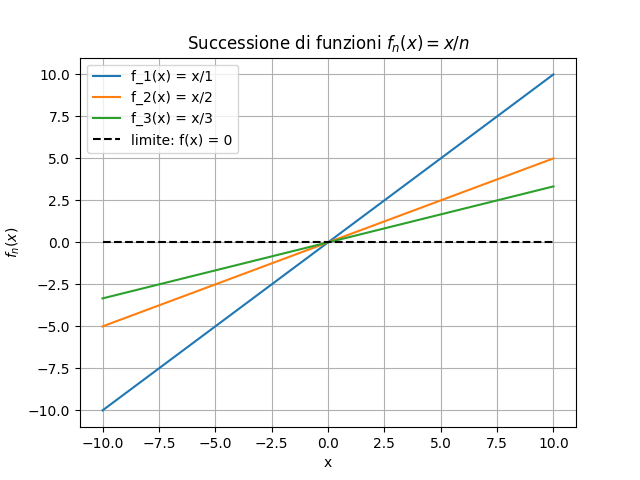
\includegraphics[width=0.5\textwidth]{./img/succ_funz_1.png}
    \caption{Grafico della successione di funzioni
    $f_n(x)=\frac{x}{n}$.}
    \label{fig:succ_funz_1}
\end{figure}

\end{example}


\begin{oss}

Viene naturale dunque domandarsi se esista una nozione di limite
per una successione di funzioni.

Fissato un $x$, la successione $f_n(x)$ è una successione numerica,
dunque posso definirne il limite

\[
\lim_{n\to\infty} f_n(x).
\]

\end{oss}


\subsection{Convergenza puntuale}

\begin{definition}

Diremo che la successione di funzioni $f_n(x)$
\textbf{converge puntualmente} alla funzione

\[
f : I \subseteq \mathbb{R} \to \mathbb{R}
\]

se

\[
\forall x \in I
\qquad
\lim_{n\to\infty} f_n(x) = f(x).
\]

Equivalentemente:
\begin{align*}
&\forall x \in I, \forall \epsilon > 0 \exists \nu_{\epsilon,x}> 0 : | f_{n} (x) - f(x) | < \epsilon \forall n > \nu_{\epsilon, x} \\
& \text{ e scriveremo } \lim_{n} f_{n} ( x) = f(x), x \in I    
\end{align*}

oppure: \(f_{n}(x) \conv{P} f(x)\) in I

\end{definition}


\begin{example}
    \[
    f_{n} (x) = \frac{x}{n} \forall x \in \R \conv{P} f(x) = 0 \forall x \in \R
    \]

    \[
    f_{n} (x) = \frac{n+x}{n+ (-1)^n + \sqrt{ n }} \conv{P} f(x) = 1
    \]
\end{example}

\begin{example}
    \[
    f_n(x) = \frac{n}{n^2x + 2n - 1}.
    \]

    Se $x=0$, il termine $n^2x$ si annulla e dunque devo distinguere
    il caso $x=0$ dal caso $x\neq 0$.

    \[
    \lim_{n\to\infty} f_n(x) =
    \begin{cases}
    0, & x \in \mathbb{R}\setminus\{0\},\\
    \dfrac{1}{2}, & x=0
    \end{cases}
    \]
\end{example}

\begin{example}
    \[
    f_{n}(x) = x^n, \; x \in [0,1]
    \]
    \[
    f_{n}(x) \conv{P} f(x) = \begin{cases}
        0, & x \in [0,1[,\\
        1, & x=1
    \end{cases}
    \]
    \begin{figure}[H]
    \centering
    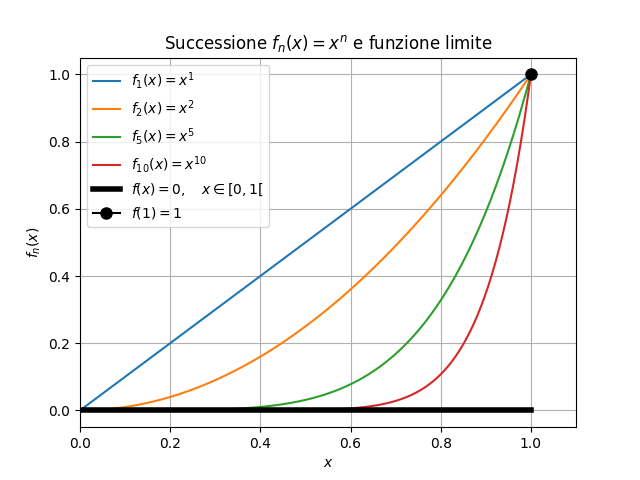
\includegraphics[width=0.5\textwidth]{./img/succ_funz_2.png}
    \caption{Grafico della successione di funzioni
    $f_n(x)=x^n$.}
    \label{fig:succ_funz_2}
    \end{figure}

\end{example}


    \begin{example}
        \[
        f_{n}(x) = x^\frac{1}{n}, \; x \in [0,1]
        \]
        \[
        f_{n}(x)\conv{P}f(x) = \begin{cases}
            1, & x \in ]0,1]\\
            0, & x =0
        \end{cases}
        \]
        \begin{figure}[H]
    \centering
    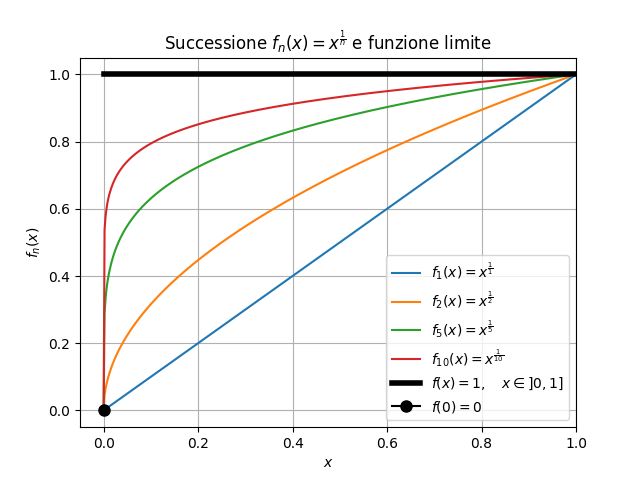
\includegraphics[width=0.5\textwidth]{./img/succ_funz_3.png}
    \caption{Grafico della successione di funzioni
    $f_n(x)=x^\frac{1}{n}$.}
    \label{fig:succ_funz_3}
    \end{figure}
        
    \end{example}

\subsection{Convergenza uniforme}

    \begin{definition}
        Sia \(f_{n}: I \sube \R \to \R, \; \forall n \in \N\)
        Diremo che \(f_{n}(x)\) \textbf{Converge Uniformemente} alla funzione \(f: I \sube \R \to \R\) e scriveremo: \(f_{n}(x)\conv{U}f(x)\) in \(I\)
        se \[\forall \epsilon > 0 \exists \nu_{\epsilon}>0 : |f_{n}(x)-f(x)| < \epsilon \, \forall n > \nu_{\epsilon}, \forall x \in I \iff\]
        \[
        \iff \forall \epsilon>0 \exists \nu_{\epsilon}>0 : \sup_{I}|f_{n}(x)-f(x)| <\epsilon \forall n > \nu_{\epsilon} \iff \lim_{n} \sup_{I}|f_{n}(x)-f(x)| = 0 \implies \lim_{n} M_{n} = 0
        \]
    \end{definition}

    \begin{example}
        \[
        f_{n} = \frac{x}{n} \conv{P} 0 \forall x\in \R \; U:?
        \]
        \[
        \sup_{\R} | \frac{x}{n} - 0| = \sup_{\R} \frac{|x|}{n} = \frac{1}{n} \sup_{\R} |x| = +\infty \implies \text{Non è Uniformemente Convergente}
        \] 
        È Unif Conv in ogni intervallo che non include una "semiretta".
    \end{example}
    \begin{example}
        \[
    f_{n}(x) = x^n, \; x \in [0,1]
    \]
    \[
    f_{n}(x) \conv{P} f(x) = \begin{cases}
        0, & x \in [0,1[,\\
        1, & x=1
    \end{cases}
    \]
    U:?
    \[
    \sup_{[0,1]} |x^n - f(x)| = 1 \not \to 0 \implies \text{Non è Unif Conv}
    \]
    È Unif Conv in \([0,b] \; 0<b<1\) 
    \end{example}

\subsection{Teorema di Continuità del Limite}
\begin{theorem}[Teo di Continuità del Limite]
    Sia \(f_{n}: I \sube\R \to \R \forall n\), una successione di funzioni continue.
    Sia \(f_{n}\conv{U} f\) in \(I\).
    Allora \(f\) è continua in I (\pencilnote{Non vale l'inversa, si pensi a \(f_{n}=\frac{x}{n}\conv{P}f=0\)}) ovvero:
    \[
    \forall x_{0} \in I \text{ si ha } \lim_{x\to x_{0}} f(x) = \lim_{x\to x_{0}}(\lim_{n\to +\infty} f_{n}(x))= f(x_{0}) =\lim_{n\to +\infty }(\lim_{x\to x_{0}} f_{n}(x)) = \lim_{n \to +\infty }f_{n}(x_{0})
    \]
    \pencilnote{Se mi voglio restringere per trovare un intervallo di uniformità, dovrò prenderne uno dove \(f(x)\) è continua.}
\end{theorem}

\begin{proof}
    Sia \(x_{0}\in I\) (\pencilnote{avendo fissato \(x_{0}\implies\)la def di continuità è \(\forall x_{0} \in I \forall \epsilon>0 \exists \delta_{\epsilon,x_{0}}\dots, \) avendolo fissato, posso scrivere \(\forall\epsilon>0\), vogliamo dimostrare che \(f\) è continua in \(x_{0}\).})
    Consideriamo le Hp:
    \begin{enumerate}
        \item \(f_{n}\) è continua in \(x_{0} \iff \forall \epsilon > 0 \exists \delta_{n}>0 : \forall x \in I, |x-x_{0}| < \delta_{n} \implies |f_{n}(x)-f_{n}(x_{0})|<\epsilon\)
        \item \(f_{n}\conv{U}f \text{ in } I \iff \forall \epsilon > 0 \exists \nu_{\epsilon}>0: |f_{n}(x)-f(x)|<\epsilon \forall n>\nu_{\epsilon}, \forall x \in I\)
    \end{enumerate}
    Th: \(\forall \epsilon>0 \exists \delta_{\epsilon}>0 : \forall x \in I, |x-x_{0}|<\delta_{\epsilon}\implies |f(x)-f(x_{0})|<\epsilon\)
    Sia \(\epsilon'>0\) e consideriamo (fissato un \(\overline{n}\) che superi la soglia)
    \begin{align*}
    &|f(x)-f(x_{0})|=|f(x)+f_{\overline{n}}(x)-f_{\overline{n}}(x)+f_{\overline{n}}(x_{0})-f_{\overline{n}}(x_{0})-f(x_{0})| \underset{\text{Dis. Tri.}}{\leq} \\ 
    &\leq \underset{(1)}{|f(x)-f_{\overline{n}}(x)|}+\underset{(2)}{|f_{\overline{n}}(x)-f_{\overline{n}}(x_{0})|}+\underset{(3)}{|f_{\overline{n}}(x_{0})-f(x_{0})|} < 3\epsilon'
    \end{align*}
\begin{oss}
\begin{enumerate}
    \item è minore di \(\epsilon'\) perchè \(f_{n}\conv{U}f\)
    \item fissato un \(\overline{n}\) se \(|x-x_{0}|<\delta_{\overline{n}}\equiv \delta_{\epsilon}\implies |f_{\overline{n}}(x)-f_{\overline{n}}(x_{0})|<\epsilon'\)
    \item analogo a (1) poichè essendo UNIFORME, vale \(\forall x \in I\)
\end{enumerate}
\end{oss}
Segue quindi \(|f(x)-f(x_{0})|<3\epsilon' \equiv \epsilon\), dunque vale la tesi.
\end{proof}


\subsection{Passaggio al limite sotto il segno di integrale}
\pencilnote{Immaginiamo di voler calcolare \(\int_{a}^{b}f(x)dx \implies \) per assicurare l'integrabilità mi serve che \(f_{n}\conv{U}f\), a questo punto \(\int_{a}^{b}\lim_{n}f_{n}(x)dx = \int_{a}^{b}f(x)dx\).

Ci chiediamo dunque se sia possibile cambiare l'ordine degli operatori, ovvero: \(\lim_{n}\int_{a}^{b}f_{n}(x)dx = \int_{a}^{b}\lim_{n}f_{n}(x)dx\)}

\begin{theorem}[Teorema Passaggio al limite sotto il segno di integrale]
    \begin{itemize}
        \item Sia \(f_{n}: [a,b]\sube\R \to \R\) continua \(\forall n\)
        \item Sia \(f_{n}\conv{U} f\) in \([a,b]\)
    \end{itemize}
    \pencilnote{(Con queste due hp mi sono assicurato la continuità di \(f\))}
    Allora: 
    \[
    \lim_{n} \int_{a}^{b} f_{n}(x) dx = \int_{a}^{b} \lim_{n} f_{n}(x) dx = \int_{a}^{b} f(x) dx
    \]
    \pencilnote{Non vale \((\impliedby)\), ovvero può valere il passaggio ma non la uniforme convergenza.}
\end{theorem}
\begin{proof}
    \pencilnote{Sia \(I_{n} = \int_{a}^{b} f_{n} (x) dx\), essa rappresenta la successione degli integrali, che essendo definiti, sono una successione numerica.}
    Per dimostrare che \(I_{n}\to I\) useremo il Teorema dei carabinieri:
    \[
    0\leq |I_{n} - I| \leq | \int_{a}^{b} f_{n}(x) - f(x) dx| \leq \int_{a}^{b} |f_{n}(x) - f(x)| dx \leq (\max_{[a,b]}|f_{n}(x) - f(x)|)(b-a)
    \]
    \pencilnote{Il massimo esiste perchè la differenza è continua in un compatto}
    A questo punto, considerando che il max esiste, esso è il sup. Sfruttiamo l'unif conv che ci dice che se \(n \to +\infty \implies sup \to 0 \) dunque:
    \[
    0 \leq \lim_{n} |I_{n} -I| \leq \lim_{n} (\max_{[a,b]}|f_{n}(x) - f(x)|)(b-a)
    \]
    Per il teo dei carabinieri, si ha che \(I_{n}\to I\)
\end{proof}


\begin{example}
    Sia \(f_{n}(x) = nx(1-x^2)^n,\; x\in[0,1]\)
    \(f_{n}(x)\conv{P}f(x)\equiv 0\) \pencilnote{è continua quindi per quello che sappiamo (escluso questo teorema), potrebbe essere unif.}
    Se integrando \(f(x)\), il valore risulta diverso da \(\lim_{n}\int_{0}^{1}f_{n}(x) dx\), allora la convergenza non è uniforme.
    \[
    \int_{0}^{1} 0 dx = 0
    \]
    \[
    \begin{aligned}
    \lim_{n\to\infty}\int_0^1 n(1-x^2)^n x\,dx
    &=\lim_{n\to\infty}\frac {n}{2}\int_0^1(1-x^2)^n2x\,dx\\
    &=\lim_{n\to\infty}\frac {n}{2}\int_0^1u^n\,du
    =\lim_{n\to\infty}\frac {n}{2}\left[\frac{u^{n+1}}{n+1}\right]_0^1\\
    &=\lim_{n\to\infty}\frac{n}{2(n+1)}
    =\boxed{\frac{1}{2}},
    \end{aligned}
    \]
    dunque la conv non è uniforme.    
\end{example}

\begin{example}
    \(f_{n}(x)=nxe^{-nx}, x \in[0,1]\)
    \pencilnote{Questo esempio dimostra che non vale l'inverso. Ovvero vale il passaggio ma non vi è unif conv.}
    \(f_{n}(x)\conv{P}f(x)\equiv 0\)
    \[
    \int_{0}^{1} f(x) dx = 0
    \]
    \[
    \lim_{n} \int_{0}^{1}nx e^{-nx} dx = \dots = \lim_{n} \left. (e^{-nx} (x+\frac{1}{n}))\right|_{1}^0 = 0
    \]
    Verifichiamo sia uniforme:
    \[
    |nx e^{-nx}|= nxe^{-nx} \implies \sup_{[0,1]} (nxe^{-nx}) = \text{\pencilnote{fai derivata e trovi max}} = \frac{1}{e} \implies \lim_{n} \sup = \frac{1}{e}
    \]
    Quindi \(f_{n}\) non conv unif.    
    
\end{example}


\subsection{Passaggio al limite sotto il segno di derivata}
\begin{theorem}[Teorema Passaggio al limite sotto il segno della derivata]
    \begin{itemize}
        \item Sia \(f_{n}:[a,b]\to \R, f_{n} \in C^1 ([a,b])\) \pencilnote{L'appartenenza a \(C^1\) non è un'hp necessaria ma facilita la dimostrazione}
        \item Sia \(x_{0}\in [a,b]: \lim_{n} f_{n}(x_{0})=l \in \R\) \pencilnote{(è conv almeno in un punto)}
        \item Sia \(g:[a,b]\to \R : f_{n}' (x) \conv{U} g(x) \text{ in } [a,b]\) \pencilnote{(\(f_{n}'\) è continua per Hp, g lo è per teo di continuità del limite)}
    \end{itemize}
    Allora:
    \begin{enumerate}
        \item \(f_{n} \conv{U} f\) in \([a,b]\)
        \item \(f\in C^1 ([a,b])\) e \(f'(x) = g(x) \iff f'(x) = \frac{d}{dx} (\lim_{n} f_{n}(x)) = \lim_{n}(\frac{d}{dx} f_{n} (x))= \lim_{n}f_{n}'(x) = g(x)\)
    \end{enumerate}
\end{theorem}
\begin{proof}
    \begin{enumerate}
        \item Costruiamo \(f\). Poiché \(f_{n}\in C^1([a,b])\), vale
        \[
        f_{n}(x) = f_{n}(x_{0}) + \int_{x_{0}}^{x} f_{n}'(t)\,dt
        \]
        \pencilnote{Posso integrare questo perché \(f_{n}'\) è continua per Hp.}
        Passando al limite per \(n\to+\infty\):
        \[
        f_{n}(x) \conv{P} l + \int_{x_{0}}^{x} \lim_{n} f_{n}'(t)\,dt = l + \int_{x_{0}}^{x} g(t)\,dt = f(x)
        \]
        \pencilnote{Il limite di \(f_{n}(x_{0})\) esiste per Hp. Poiché \(f_{n}'\conv{U} g\), posso usare il teorema di passaggio al limite sotto il segno di integrale.}
        \item Verifichiamo che vale il passaggio al limite sotto la derivata (Th 2).
        Per costruzione \(f(x) = l + \int_{x_{0}}^{x} g(t)\,dt\) con \(g\) continua, dunque per il teorema fondamentale del calcolo integrale \(f\) è derivabile e
        \[
        f'(x) = g(x),
        \]
        che è continua: quindi \(f\in C^1([a,b])\). Inoltre, per Hp, \(f_{n}'\conv{U} g = f'\).
        \item Verifichiamo che \(f_{n}\conv{U} f\) (Th 1). Per ogni \(x\in[a,b]\):
        \begin{align*}
        0 \leq |f_{n}(x)-f(x)| &= \left| f_{n}(x_{0}) - l + \int_{x_{0}}^{x} \big(f_{n}'(t) - g(t)\big)\,dt \right| \leq \\
        &\leq |f_{n}(x_{0}) - l| + \int_{x_{0}}^{x} |f_{n}'(t) - g(t)|\,dt \leq \\
        &\leq |f_{n}(x_{0}) - l| + \max_{[a,b]} |f_{n}'(x) - g(x)|\,(b-a)
        \end{align*}
        Poiché \(f_{n}'\conv{U}g\) e \(f_{n}(x_{0})\to l\), il membro di destra tende a \(0\) e non dipende da \(x\). Per il teorema dei carabinieri \(|f_{n}(x)-f(x)|\to 0\) \(\forall x\in[a,b]\); passando al sup, otteniamo che la convergenza è uniforme.
    \end{enumerate}
\end{proof}

\begin{example}
    Sia \(f_{n}(x)=\sqrt{x^{2}+\frac{1}{n}}, \; x\in\R\). Osserviamo che \(f_{n}\in C^{\infty}(\R)\) e che \(f_{n}\conv{P} f(x)=|x|\).
    La convergenza è uniforme:
    \[
    \left|\sqrt{x^{2}+\tfrac{1}{n}} - |x|\right| = \sqrt{x^{2}+\tfrac{1}{n}} - |x| = \frac{\frac{1}{n}}{\sqrt{x^{2}+\frac{1}{n}}+|x|} \leq \frac{\frac{1}{n}}{\frac{1}{\sqrt{n}}} = \frac{1}{\sqrt{n}} \to 0
    \]
    Dunque \(f_{n}\conv{U} f\), ma \(f(x)=|x|\) non è derivabile in \(0\): la convergenza uniforme di \(f_{n}\) non implica la derivabilità del limite. Ovvero, il limite di funzioni \(C^{\infty}\) può non essere nemmeno \(C^1\).
\end{example}

\begin{example}
    Sia \(f_{n}(x)=\frac{\sin(nx)}{n}\) in \(\R\), \(f_{n}\in C^{\infty}(\R)\).
    Si ha \(f_{n}\conv{P} f\equiv 0\) e la convergenza è uniforme, perché
    \[
    \left|\frac{\sin(nx)}{n}\right| = \frac{|\sin(nx)|}{n} \leq \frac{1}{n}\to 0 .
    \]
    \(f\) è derivabile. Possiamo dire che vale il passaggio? Le Hp 1 e 2 sono verificate, e l'Hp 3?
    \[
    f_{n}'(x)=\cos(nx)
    \]
    Questa è una successione che in generale non ammette limite. Inoltre, anche dove il limite esiste (ad esempio in \(x=0\)), vale \(f_{n}'(0)=1\to 1\), mentre \(f'(x)=0\).
    Ergo non vale il passaggio.
\end{example}

\begin{example}
    Sia \(f_{n}(x)=\frac{x}{1+n^{2}x^{2}}, \; x\in[0,1]\), \(f_{n}\in C^{\infty}([0,1])\).
    Si ha \(f_{n}\conv{P} f\equiv 0\). Inoltre
    \[
    f_{n}'(x)=\frac{1-n^{2}x^{2}}{(1+n^{2}x^{2})^{2}}
    \]
    e \(f_{n}'(x)\geq 0 \iff 1-n^{2}x^{2}\geq 0 \iff x\leq \frac{1}{n}\).
    Quindi il massimo di \(f_{n}\) è in \(x=\frac{1}{n}\) e
    \[
    \sup_{[0,1]} f_{n}(x) = f_{n}\left(\tfrac{1}{n}\right) = \frac{1}{2n}\to 0 \implies f_{n}\conv{U} f .
    \]
    Vale il passaggio? \(f'(x)=0\), ma
    \[
    f_{n}'(x)\conv{P}\begin{cases} 1 & x=0 \\ 0 & x\neq 0 \end{cases}
    \]
    che è discontinua: dunque \(f_{n}'\) non può convergere uniformemente (altrimenti il limite sarebbe continuo per il teorema di continuità del limite) e infatti non vale il passaggio, perché \(\lim_{n}f_{n}'(0)=1\neq 0=f'(0)\).
\end{example}


\subsection{Convergenza uniforme e discontinuità}
Finora abbiamo parlato di conservazione della continuità. La convergenza uniforme conserva anche la discontinuità?

\begin{oss}
    La convergenza uniforme \textbf{non} conserva la discontinuità: una successione di funzioni discontinue può convergere uniformemente a una funzione continua.
\end{oss}

\begin{example}
    Sia
    \[
    f_{n}(x)=\begin{cases} \frac{1}{n} & x\in\mathbb{Q} \\ 0 & x\in\R\setminus\mathbb{Q} \end{cases}
    \]
    Ogni \(f_{n}\) è discontinua in ogni punto per la densità di \(\mathbb{Q}\) in \(\R\).
    Si ha \(f_{n}\conv{P}0\) in \(\R\) e \(f_{n}\conv{U}0\) in \(\R\) \pencilnote{(per dimostrare l'uniforme basta osservare che il sup è \(\frac{1}{n}\to 0\))}.
\end{example}


\subsection{Criterio di Cauchy}
\subsubsection{Criterio di Cauchy per la convergenza puntuale}
\begin{theorem}[Criterio di Cauchy per la convergenza puntuale]
    Sia \(f_{n}:I\sube\R\to\R\) \(\forall n\in\mathbb{N}\) e sia \(f:I\sube\R\to\R\).
    \[
    f_{n}\conv{P}f \text{ in } I \iff \forall x\in I,\; \forall\epsilon>0\; \exists \nu_{\epsilon,x}>0 : |f_{n}(x)-f_{m}(x)|<\epsilon \quad \forall n,m>\nu_{\epsilon,x}
    \]
\end{theorem}
\begin{proof}
    Segue dal criterio di Cauchy per le successioni numeriche, poiché fissata una \(x\in I\), \(f_{n}(x)\) è una successione numerica.
\end{proof}

\subsubsection{Criterio di Cauchy per la convergenza uniforme}
\begin{theorem}[Criterio di Cauchy per la convergenza uniforme]
    Sia \(f_{n}:I\sube\R\to\R\) \(\forall n\in\mathbb{N}\) e sia \(f:I\sube\R\to\R\).
    \[
    f_{n}\conv{U}f \text{ in } I \iff \forall\epsilon>0\; \exists \nu_{\epsilon}>0 : |f_{n}(x)-f_{m}(x)|<\epsilon \quad \forall n,m>\nu_{\epsilon},\; \forall x\in I
    \]
    \pencilnote{Ogni volta che fisso una \(x\) in \(I\), ottengo una successione di Cauchy con lo stesso \(\nu\).}
\end{theorem}
\begin{proof}
    \((\implies)\) Se \(f_{n}\conv{U}f\) in \(I\), allora \(\forall\epsilon>0\; \exists\nu_{\epsilon}: |f_{n}(x)-f(x)|<\epsilon\) \(\forall n>\nu_{\epsilon}\), \(\forall x\in I\).
    Allora
    \[
    |f_{n}(x)-f_{m}(x)| = |f_{n}(x)-f(x)-f_{m}(x)+f(x)| \underset{\text{Dis. Tri.}}{\leq} |f_{n}(x)-f(x)|+|f_{m}(x)-f(x)| < 2\epsilon
    \]
    da cui la tesi. Se \(n,m>\nu_{\epsilon}\) e \(\forall x\in I\) otteniamo che i moduli sono \(<\epsilon\) per Hp.

    \((\impliedby)\) Supponiamo che \(\forall\epsilon>0\; \exists\nu_{\epsilon}>0: |f_{n}(x)-f_{m}(x)|<\epsilon\) \(\forall n,m>\nu_{\epsilon},\; \forall x\in I\) \hfill \((*)\) \pencilnote{(vale la condizione di Cauchy)}

    Fissata una \(x\in I\), la successione \(f_{n}(x)\) è una successione numerica di Cauchy che converge a un certo numero reale \(f(x)\). Possiamo quindi scrivere
    \[
    |f_{n}(x)-f(x)| = \lim_{m\to+\infty} |f_{n}(x)-f_{m}(x)|
    \]
    Dunque, passando al limite per \(m\to+\infty\) nella condizione di Cauchy \((*)\), otteniamo
    \[
    \forall\epsilon>0\; \exists\nu_{\epsilon}>0: |f_{n}(x)-f(x)|\leq\epsilon \quad \forall n>\nu_{\epsilon},\; \forall x\in I,
    \]
    cioè \(f_{n}\conv{U}f\) in \(I\).
\end{proof}

% !TeX root = ../analisi_2.tex

\section{Serie di funzioni}

\subsection{Definizioni e convergenza}

\begin{definition}
Sia $f_n : I \subseteq \mathbb{R} \to \mathbb{R}$, $\forall n \in \mathbb{N}$, una successione di funzioni. Si chiama \textbf{serie di funzioni} di termine generale $f_n(x)$, e si indica con
$$\sum_{n=1}^{+\infty} f_n(x),$$
la successione di funzioni delle \textbf{somme parziali} definita da
$$S_1(x) = f_1(x), \quad S_2(x) = S_1(x) + f_2(x), \quad \dots, \quad S_n(x) = S_{n-1}(x) + f_n(x).$$
\begin{itemize}
\item Diremo che la serie \textbf{converge puntualmente} alla somma $S(x)$ in $I$ se $S_n(x) \xrightarrow{\text{P}} S(x)$ in $I$.
\item Diremo che la serie \textbf{converge uniformemente} alla somma $S(x)$ in $I$ se $S_n(x) \xrightarrow{\text{U}} S(x)$ in $I$.
\end{itemize}
\end{definition}\begin{oss}
La convergenza uniforme della serie implica la convergenza puntuale della serie, ma non vale il viceversa:
$$\text{Conv. uniforme} \implies \text{Conv. puntuale}, \qquad \text{Conv. uniforme} \not\Longleftarrow \text{Conv. puntuale}.$$
\end{oss}\begin{example}[Serie geometrica di funzioni]
Consideriamo la serie
$$\sum_{n=0}^{\infty} x^n, \quad x \in \mathbb{R}.$$
\begin{itemize}
\item \textbf{Convergenza puntuale:} da quanto noto sulla serie geometrica numerica, la serie converge puntualmente in $]-1, 1[$ alla funzione somma
$$S(x) = \frac{1}{1 - x}.$$
\item \textbf{Convergenza uniforme:} calcoliamo l'estremo superiore dello scarto in $]-1, 1[$ \pencilnote{(ricordando che $S_n(x)$ è la somma parziale di una progressione geometrica)}:
$$\sup_{]-1, 1[} \vert{}S_n(x) - S(x)\vert{} = \sup_{]-1, 1[} \left\vert{} \frac{1 - x^{n+1}}{1 - x} - \frac{1}{1 - x} \right\vert{} = \sup_{]-1, 1[} \left\vert{} -\frac{x^{n+1}}{1 - x} \right\vert{} = \sup_{]-1, 1[} \frac{\vert{}x\vert{}^{n+1}}{1 - x} = +\infty$$
\pencilnote{(per $x \to 1^-$ il rapporto diverge a $+\infty$)}, quindi la serie \textbf{non converge uniformemente} in $]-1, 1[$.Per avere convergenza uniforme è necessario allontanarsi da $x = 1$, restringendosi a intervalli del tipo $\vert{}x\vert{} \le r$ (ovvero $[-r, r]$) con $0 < r < 1$.
\end{itemize}
\end{example}\begin{example}[Serie a segno alterno]
Studiamo la serie
$$\sum_{n=1}^{\infty} (-1)^n \frac{x^2 + n}{n^2}, \quad x \in [-1, 1].$$
\begin{itemize}
\item \textbf{Convergenza puntuale:} per ogni fissato $x \in [-1, 1]$, la serie converge puntualmente per il criterio di Leibniz.
\item \textbf{Convergenza uniforme:} sfruttiamo la stima del resto fornita dal criterio di Leibniz, secondo cui $\vert{}S_n(x) - S(x)\vert{} \le a_{n+1}(x)$ (il primo termine trascurato):
$$\sup_{[-1, 1]} \vert{}S_n(x) - S(x)\vert{} \le \sup_{[-1, 1]} a_{n+1}(x) = \sup_{[-1, 1]} \frac{x^2 + n + 1}{(n+1)^2} = \frac{n + 2}{(n+1)^2} \xrightarrow{n \to \infty} 0$$
\pencilnote{(dove l'estremo superiore è assunto per $x = \pm 1$)}. Pertanto la serie \textbf{converge uniformemente} in $[-1, 1]$.
\end{itemize}
\end{example}

\subsection{Convergenza assoluta}

\begin{definition}
Sia $f_n : I \subseteq \mathbb{R} \to \mathbb{R}$ per ogni $n \in \mathbb{N}$. La serie $\sum_{n=1}^{\infty} f_n(x)$ \textbf{converge assolutamente} in $I$ se converge puntualmente in $I$ la serie dei moduli
$$\sum_{n=1}^{\infty} \vert{}f_n(x)\vert{}.$$
\end{definition}\begin{example}
Riprendiamo il termine generale $f_n(x) = (-1)^n \frac{x^2 + n}{n^2}$ per $x \in [-1, 1]$. Passando ai moduli si ha
$$\vert{}f_n(x)\vert{} = \frac{x^2 + n}{n^2}.$$
Confrontando asintoticamente con $\frac{1}{n}$:
$$\lim_{n \to \infty} \frac{\frac{x^2 + n}{n^2}}{\frac{1}{n}} = \lim_{n \to \infty} \frac{n^2 + x^2 n}{n^2} = 1,$$
dunque $\sum_{n=1}^{\infty} \frac{x^2 + n}{n^2}$ \textbf{diverge} per confronto con la serie armonica con $\alpha = 1$.
\end{example}\begin{oss}
La serie dell'esempio precedente converge uniformemente in $[-1, 1]$ ma non converge assolutamente. Di conseguenza, non sussiste alcuna implicazione generale tra convergenza assoluta e convergenza uniforme.
\end{oss}

\subsection{Criteri di Cauchy per le serie}

Sia $f_n : I \subseteq \mathbb{R} \to \mathbb{R}$ una successione di funzioni.\begin{theorem}[Criterio di Cauchy per la convergenza puntuale]
La serie $\sum_{n=1}^{\infty} f_n(x)$ converge puntualmente in $I$ se e solo se
$$\forall x \in I, \ \forall \varepsilon > 0 \ \exists \nu_{\varepsilon, x} > 0 : \quad \vert{}S_{n+p}(x) - S_n(x)\vert{} = \vert{}f_{n+1}(x) + \dots + f_{n+p}(x)\vert{} < \varepsilon \quad \forall p \in \mathbb{N}, \ \forall n > \nu_{\varepsilon, x}.$$
\end{theorem}\begin{proof}
Discende direttamente dal criterio di Cauchy per le serie numeriche applicato punto per punto per ogni $x \in I$ fissato.
\end{proof}\begin{theorem}[Criterio di Cauchy per la convergenza uniforme]
La serie $\sum_{n=1}^{\infty} f_n(x)$ converge uniformemente in $I$ se e solo se
$$\forall \varepsilon > 0 \ \exists \nu_{\varepsilon} > 0 : \quad \vert{}S_{n+p}(x) - S_n(x)\vert{} = \vert{}f_{n+1}(x) + \dots + f_{n+p}(x)\vert{} < \varepsilon \quad \forall p \in \mathbb{N}, \ \forall n > \nu_{\varepsilon}, \ \forall x \in I.$$
\end{theorem}Dalla condizione di Cauchy segue la \textbf{condizione necessaria per la convergenza di una serie}:\begin{prop}[Condizione necessaria]
Sia $f_n : I \subseteq \mathbb{R} \to \mathbb{R}$ per ogni $n \in \mathbb{N}$.
\begin{itemize}
\item Se $\sum_{n=1}^{\infty} f_n(x)$ converge puntualmente in $I$, allora $f_n(x) \xrightarrow{\text{P}} 0$ in $I$.
\item Se $\sum_{n=1}^{\infty} f_n(x)$ converge uniformemente in $I$, allora $f_n(x) \xrightarrow{\text{U}} 0$ in $I$.
\end{itemize}
\end{prop}\begin{proof}
Dimostriamo il caso uniforme. Poiché $\sum_{n=1}^{\infty} f_n(x)$ converge uniformemente in $I$, verifica la condizione di Cauchy uniforme:
$$\forall \varepsilon > 0 \ \exists \nu_{\varepsilon} > 0 : \quad \vert{}f_{n+1}(x) + \dots + f_{n+p}(x)\vert{} < \varepsilon \quad \forall n > \nu_{\varepsilon}, \ \forall p \in \mathbb{N}, \ \forall x \in I.$$
Scelto $p = 1$, si ottiene $\vert{}f_{n+1}(x)\vert{} < \varepsilon$ per ogni $n > \nu_{\varepsilon}$ e per ogni $x \in I$, ovvero $\sup_{I} \vert{}f_{n+1}(x) - 0\vert{} \to 0$, cioè $f_n \xrightarrow{\text{U}} 0$ in $I$.
\end{proof}

\subsection{Totale convergenza}

Per formulare delle condizioni sufficienti alla convergenza uniforme è necessario introdurre una nuova nozione di convergenza.\begin{definition}
Sia $f_n : I \subseteq \mathbb{R} \to \mathbb{R}$ per ogni $n \in \mathbb{N}$. Diremo che $\sum_{n=1}^{\infty} f_n(x)$ \textbf{converge totalmente} in $I$ se esiste una successione numerica $M_n > 0$ tale che:
\begin{enumerate}
\item $\vert{}f_n(x)\vert{} \le M_n \quad \forall n \in \mathbb{N}, \ \forall x \in I$;
\item la serie numerica $\sum_{n=1}^{\infty} M_n$ converge.
\end{enumerate}
\end{definition}Nella pratica, la successione $M_n$ può essere scelta ponendo $M_n = \sup_{I} \vert{}f_n(x)\vert{}$, che coincide con la stessa quantità calcolata nella verifica della condizione necessaria per la convergenza uniforme di una serie.\begin{oss}[Implicazioni]
$$\text{Convergenza totale} \implies \text{Convergenza assoluta} \implies \text{Convergenza puntuale}.$$
Infatti, per confronto, la serie dei moduli $\sum_{n=1}^{\infty} \vert{}f_n(x)\vert{}$ è maggiorata dalla serie numerica convergente $\sum_{n=1}^{\infty} M_n$, e la convergenza assoluta implica a sua volta la convergenza semplice (puntuale).
\end{oss}\begin{theorem}[Criterio di Weierstrass]
Sia $f_n : I \subseteq \mathbb{R} \to \mathbb{R}$ per ogni $n \in \mathbb{N}$. Se la serie $\sum_{n=1}^{\infty} f_n(x)$ \textbf{converge totalmente} in $I$, allora $\sum_{n=1}^{\infty} f_n(x)$ \textbf{converge uniformemente} in $I$.
\end{theorem}\begin{proof}
Si sfrutta il criterio di Cauchy uniforme. Poiché per ipotesi la serie converge totalmente in $I$, esiste una successione $M_n > 0$ tale che:
\begin{enumerate}
\item $\vert{}f_n(x)\vert{} \le M_n \quad \forall n \in \mathbb{N}, \ \forall x \in I$;
\item $\sum_{n=1}^{\infty} M_n$ converge, dunque per il criterio di Cauchy per le serie numeriche si ha che
$$\forall \varepsilon > 0 \ \exists \nu_{\varepsilon} > 0 : \quad M_{n+1} + \dots + M_{n+p} < \varepsilon \quad \forall p \in \mathbb{N}, \ \forall n > \nu_{\varepsilon}.$$
\end{enumerate}
Mostriamo che vale la condizione di Cauchy uniforme. Fissato $\varepsilon > 0$, per ogni $p \in \mathbb{N}$, per ogni $n > \nu_{\varepsilon}$ e per ogni $x \in I$, stimiamo lo scarto $\vert{}S_{n+p}(x) - S_n(x)\vert{}$:
$$\vert{}f_{n+1}(x) + \dots + f_{n+p}(x)\vert{} \le \vert{}f_{n+1}(x)\vert{} + \dots + \vert{}f_{n+p}(x)\vert{} \le M_{n+1} + \dots + M_{n+p} < \varepsilon,$$
dove si sono usate nell'ordine la disuguaglianza triangolare, la prima ipotesi di maggiorazione e la condizione di Cauchy sulla serie $\sum M_n$. Pertanto la serie converge uniformemente in $I$.
\end{proof}\begin{oss}
Non vale il viceversa del criterio di Weierstrass: la convergenza uniforme non implica la convergenza totale. L'esempio della serie a segno alterno $\sum_{n=1}^{\infty} (-1)^n \frac{x^2 + n}{n^2}$ in $[-1, 1]$ lo dimostra: essa converge uniformemente ma non converge assolutamente, quindi non può convergere totalmente.
\end{oss}

\subsection{Criterio di integrazione per serie}

\begin{theorem}[Integrazione per serie]
Sia $f_n : [a, b] \to \mathbb{R}$ integrabile per ogni $n \in \mathbb{N}$. Se $\sum_{n=1}^{\infty} f_n(x)$ converge uniformemente a $S(x)$ in $[a, b]$, allora
$$\sum_{n=1}^{\infty} \int_a^b f_n(x) \, dx = \int_a^b \sum_{n=1}^{\infty} f_n(x) \, dx = \int_a^b S(x) \, dx.$$
\end{theorem}\begin{proof}
Consideriamo la successione delle somme parziali degli integrali:
$$I_n = \sum_{k=1}^{n} \int_a^b f_k(x) \, dx = \int_a^b f_1(x) \, dx + \dots + \int_a^b f_n(x) \, dx = \int_a^b \underbrace{\left[ f_1(x) + \dots + f_n(x) \right]}_{S_n(x)} \, dx.$$
\end{proof}

\subsection{Teorema di derivazione per serie}

\begin{theorem}[Derivazione per serie]
Sia $f_n : [a, b] \to \mathbb{R}$ una successione di funzioni tale che:
\begin{enumerate}
    \item $f_n \in C^1([a, b])$ per ogni $n \in \mathbb{N}$;
    \item $\sum_{n=1}^{\infty} f_n(x) \xrightarrow{\text{P}} S(x)$ in $[a, b]$;
    \item $\sum_{n=1}^{\infty} f'_n(x) \xrightarrow{\text{U}} G(x)$ in $[a, b]$.
\end{enumerate}
Allora $S(x) \in C^1([a, b])$ e
\[
S'(x) = G(x) \qquad \forall x \in [a, b].
\]
\end{theorem}

\begin{proof}
Per l'ipotesi (1), $f_n \in C^1([a, b]) \implies f'_n \in C^0([a, b])$. Per l'ipotesi (3), $\sum_{n=1}^{\infty} f'_n(x) \xrightarrow{\text{U}} G(x)$ in $[a, b]$, dunque $G(x)$ è continua su $[a, b]$ \pencilnote{(come limite uniforme di funzioni continue)}.

Applichiamo il teorema fondamentale del calcolo integrale a ciascuna $f_n$:
\[
f_n(x) = f_n(a) + \int_a^x f'_n(t) \, dt.
\]
Passando alle somme parziali di ordine $k$, si ottiene:
\[
\sum_{n=1}^{k} f_n(x) = \sum_{n=1}^{k} f_n(a) + \sum_{n=1}^{k} \int_a^x f'_n(t) \, dt.
\]
Passando al limite per $k \to +\infty$ e sfruttando il teorema di integrazione per serie sulla serie delle derivate (che converge uniformemente a $G$), segue che:
\[
S(x) = S(a) + \int_a^x G(t) \, dt
\]
\pencilnote{(dove la funzione integrale appartiene a $C^1([a, b])$ poiché $G$ è continua)}. Infine, per il teorema fondamentale del calcolo integrale, si conclude che $S \in C^1([a, b])$ e $S'(x) = G(x)$.
\end{proof}

% !TeX root = ../analisi_2.tex

\section{Serie di potenze}

\subsection{Definizione e insieme di convergenza}

\begin{definition}
Sia $\{a_n\}_{n \in \mathbb{N}_0}$ una successione numerica e sia $x_0 \in \mathbb{R}$. Si chiama \textbf{serie di potenze} di \textbf{punto iniziale} $x_0$ e \textbf{coefficienti} $a_n$ (detti anche termine generale) la seguente serie di funzioni:
\[
\sum_{n=0}^{+\infty} a_n (x - x_0)^n = a_0 + a_1 (x - x_0) + a_2 (x - x_0)^2 + \dots + a_n (x - x_0)^n + \dots, \quad x \in \mathbb{R}
\]
\pencilnote{(dove il termine generale della serie di funzioni è $f_n(x) = a_n (x - x_0)^n$)}.
\end{definition}

\begin{oss}
La serie di potenze converge sempre in almeno un punto: il suo punto iniziale $x = x_0$, dove ha per somma $a_0$.
\end{oss}

\begin{oss}
A meno di effettuare la sostituzione $y = x - x_0$, possiamo limitarci a studiare soltanto le serie di potenze centrate in $x_0 = 0$, ovvero della forma
\[
\sum_{n=0}^{\infty} a_n y^n.
\]
\end{oss}

\begin{definition}
Sia $\sum_{n=0}^{\infty} a_n x^n$ una serie di potenze. Si chiama \textbf{insieme di convergenza} della serie il seguente sottoinsieme di $\mathbb{R}$:
\[
X = \left\{ x \in \mathbb{R} \ \middle|\ \sum_{n=0}^{\infty} a_n x^n \text{ converge} \right\}.
\]
\end{definition}

\begin{oss}
L'insieme di convergenza è sempre non vuoto ($X \neq \emptyset$), poiché $0 \in X$.
\end{oss}

\begin{definition}
Si chiama \textbf{raggio di convergenza} della serie di potenze il valore
\[
\rho = \sup X.
\]
\end{definition}

\begin{oss}
Risulta sempre $\rho \ge 0$ (con $\rho \in [0, +\infty]$).
\end{oss}

\begin{example}
Consideriamo la serie geometrica $\sum_{n=0}^{\infty} x^n$.
\begin{itemize}
    \item L'insieme di convergenza puntuale è $X = ]-1, 1[$, da cui $\rho = 1$.
    \item In ogni intervallo chiuso $[-r, r]$ con $0 < r < 1$ ($\vert r \vert < 1$) si ha convergenza totale.
\end{itemize}
\end{example}

\subsection{Raggio di convergenza}

\begin{theorem}
Sia $\sum_{n=0}^{+\infty} a_n x^n$ una serie di potenze. Allora si ha:
\begin{enumerate}
    \item[(i)] Se esiste $x_1 \neq 0$ tale che $x_1 \in X$ (cioè la serie converge in $x_1$), allora la serie converge \textbf{assolutamente} per ogni $x \in ]-\vert x_1 \vert, \vert x_1 \vert[$ e \textbf{totalmente} in $[-r, r]$ per ogni $0 < r < \vert x_1 \vert$.
    \item[(ii)] Se la serie \textbf{non converge} in un certo $x_2 \in \mathbb{R}$, allora \textbf{non converge} per ogni $x \in \mathbb{R}$ tale che $\vert x \vert > \vert x_2 \vert$.
\end{enumerate}
\end{theorem}

\begin{proof}
\textbf{(i)} Sia $x_1 \neq 0$ tale che la serie converge in $x_1$, ovvero $\sum_{n=0}^{\infty} a_n x_1^n$ converge. Per la condizione necessaria di convergenza delle serie si ha
\[
a_n x_1^n \xrightarrow{n \to \infty} 0 \implies \vert a_n x_1^n \vert \le M \quad \forall n \in \mathbb{N}_0
\]
\pencilnote{(poiché ogni successione convergente è limitata)}.

Proviamo che vi è convergenza assoluta in $]-\vert x_1 \vert, \vert x_1 \vert[$. Sia $x \in \mathbb{R}$ tale che $0 \le \vert x \vert < \vert x_1 \vert$ e dimostriamo che converge la serie dei moduli $\sum_{n=0}^{+\infty} \vert a_n x^n \vert$. Poiché $x_1 \neq 0$, possiamo maggiorare il termine generale nel modo seguente:
\[
\vert a_n x^n \vert = \vert a_n x_1^n \vert \left\vert \frac{x}{x_1} \right\vert^n \le M \left( \frac{\vert x \vert}{\vert x_1 \vert} \right)^n = M \frac{\vert x \vert^n}{\vert x_1 \vert^n} \quad \forall n \in \mathbb{N}_0.
\]
Passando alle serie si ha dunque
\[
\sum_{n=0}^{+\infty} \vert a_n x^n \vert \le M \sum_{n=0}^{+\infty} \left( \frac{\vert x \vert}{\vert x_1 \vert} \right)^n,
\]
e il secondo membro converge per ogni $x$ con $\vert x \vert < \vert x_1 \vert$ in quanto serie geometrica di ragione $\frac{\vert x \vert}{\vert x_1 \vert} < 1$.

Inoltre, fissato $0 < r < \vert x_1 \vert$, per ogni $x \in [-r, r]$ (ossia $\vert x \vert \le r$) si ha
\[
\vert a_n x^n \vert \le M \left( \frac{r}{\vert x_1 \vert} \right)^n =: M_n.
\]
Poiché $\sum_{n=0}^{+\infty} M_n$ converge essendo una serie geometrica numerica di ragione $\frac{r}{\vert x_1 \vert} < 1$, la serie di potenze converge totalmente in $[-r, r]$.

\textbf{(ii)} Sia $x_2 \in \mathbb{R}$ tale che $\sum_{n=0}^{\infty} a_n x_2^n$ non converge; dobbiamo dimostrare che la serie non converge per alcun $x \in \mathbb{R}$ con $\vert x \vert > \vert x_2 \vert$.

Supponiamo, per fissare le idee, $x > 0$ \pencilnote{(il caso $x < 0$ è del tutto analogo)} con $\vert x \vert > \vert x_2 \vert$, e supponiamo \textbf{per assurdo} che la serie converga in $x$. Allora, per il punto (i), la serie dovrebbe convergere in tutto l'intervallo $]-\vert x \vert, \vert x \vert[$. Ma poiché $\vert x_2 \vert < \vert x \vert$, si ha $x_2 \in ]-\vert x \vert, \vert x \vert[$, quindi la serie convergerebbe anche in $x_2$, il che è assurdo.
\end{proof}

\begin{theorem}
Sia $\sum_{n=0}^{\infty} a_n x^n$ una serie di potenze e sia $\rho$ il suo raggio di convergenza. Allora si ha:
\begin{enumerate}
    \item[(i)] $\rho = 0 \iff$ la serie converge solo in $x = 0$ \pencilnote{(ovvero $X = \{0\}$)}.
    \item[(ii)] $\rho = +\infty \iff$ la serie converge \textbf{assolutamente} (e puntualmente) in tutto $\mathbb{R}$ e \textbf{totalmente} nei compatti $[-r, r]$ con $r > 0$ \pencilnote{(ovvero $X = \mathbb{R}$)}.
    \item[(iii)] Se $0 < \rho < +\infty$, allora la serie converge \textbf{assolutamente} in $]-\rho, \rho[$, converge \textbf{totalmente} in $[-r, r]$ per ogni $0 < r < \rho$, e \textbf{non converge} per $\vert x \vert > \rho$.
\end{enumerate}
\end{theorem}

\pencilnote{Nel caso $0 < \rho < +\infty$, l'insieme di convergenza $X$ può coincidere con $]-\rho, \rho[$, con $[-\rho, \rho]$, oppure con uno dei due intervalli semiaperti $]-\rho, \rho]$ o $[-\rho, \rho[$, a seconda del comportamento della serie agli estremi $\pm \rho$.}

\subsection{Calcolo del raggio di convergenza}

Sorgono quindi due domande naturali:
\begin{enumerate}
    \item Che cosa succede agli estremi $\pm \rho$ (anche rispetto alla convergenza uniforme)?
    \item Come si calcola il raggio di convergenza $\rho$?
\end{enumerate}

\begin{theorem}[Criterio di Hadamard]
Sia $\sum_{n=0}^{+\infty} a_n x^n$ una serie di potenze. Se esiste
\[
\lim_{n \to +\infty} \sqrt[n]{\vert a_n \vert} = \ell,
\]
allora il raggio di convergenza è dato da
\[
\rho = \begin{cases}
0 & \text{se } \ell = +\infty, \\
+\infty & \text{se } \ell = 0, \\
\dfrac{1}{\ell} & \text{se } 0 < \ell < +\infty,
\end{cases}
\]
ovvero, in forma compatta, $\rho = \dfrac{1}{\ell}$.
\end{theorem}

\pencilnote{Esempio: per la serie $\sum_{n=1}^{\infty} \frac{x^n}{n}$ si ha $a_n = \frac{1}{n}$, da cui $\frac{1}{\rho} = \lim_{n \to +\infty} \frac{1}{\sqrt[n]{n}} = 1 \implies \rho = 1$, quindi $X \supseteq ]-1, 1[$.}

\begin{proof}
Applichiamo il criterio della radice alla serie dei moduli $\sum_{n=0}^{+\infty} \vert a_n \vert \vert x \vert^n$:
\[
\lim_{n \to +\infty} \sqrt[n]{\vert a_n \vert \vert x \vert^n} = \lim_{n \to +\infty} \sqrt[n]{\vert a_n \vert} \cdot \vert x \vert = \ell \cdot \vert x \vert
\]
\pencilnote{(per ipotesi)}. Distinguiamo i tre casi possibili per $\ell$:
\begin{itemize}
    \item Se $\ell = +\infty$, allora $\ell \cdot \vert x \vert = +\infty > 1$ per ogni $x \neq 0$, dunque la serie non converge mai al di fuori dell'origine e $\rho = 0$.
    \item Se $\ell = 0$, allora $\ell \cdot \vert x \vert = 0 < 1$ per ogni $x \in \mathbb{R}$, dunque la serie converge sempre e $\rho = +\infty$.
    \item Se $0 < \ell < +\infty$, per il criterio della radice la serie converge quando $\ell \cdot \vert x \vert < 1$, ossia per $\vert x \vert < \frac{1}{\ell}$ (mentre non converge per $\vert x \vert > \frac{1}{\ell}$), da cui $\rho = \frac{1}{\ell}$.
\end{itemize}
\end{proof}

\begin{theorem}[Criterio di D'Alembert]
Sia $\sum_{n=0}^{+\infty} a_n x^n$ una serie di potenze (con $a_n \neq 0$ definitivamente). Se esiste
\[
\lim_{n \to +\infty} \left\vert \frac{a_{n+1}}{a_n} \right\vert = \ell,
\]
allora
\[
\rho = \frac{1}{\ell},
\]
dove si sottintende l'estensione dell'algebra dei limiti (ossia $\rho = +\infty$ se $\ell = 0$ e $\rho = 0$ se $\ell = +\infty$).
\end{theorem}

\begin{proof}
Ovvia, come conseguenza immediata del criterio del rapporto per le serie numeriche applicato alla serie dei moduli (oppure del legame tra criterio del rapporto e della radice).
\end{proof}

\subsection{Teorema di Abel (S.d.)}

\begin{theorem}[Teorema di Abel]
Sia $\sum_{n=0}^{+\infty} a_n x^n$ una serie di pot. e sia $0 < \rho < +\infty$ il suo raggio di conv. Se la serie conv. in $x = \rho$ (o in $x = -\rho$) allora la serie conv. \underline{uniformemente} in ogni intervallo del tipo $[y, \rho]$ (o $[-\rho, y]$) con $-\rho < y < \rho$.

Se conv. sia in $x = \rho$ che in $x = -\rho$ allora conv. unif. in $[-\rho, \rho]$.
\end{theorem}

\begin{example}
$\sum \frac{(-1)^n}{n} x^n$ \pencilnote{(con $a_n = \frac{(-1)^n}{n}$)} $\implies \frac{1}{\rho} = \lim_{n} \sqrt[n]{\vert a_n \vert} = \lim_{n} \sqrt[n]{\left\vert \frac{(-1)^n}{n} \right\vert} = 1 \implies \rho = 1 \implies$ la serie conv. punt. $]-1, 1[$ e tot. in $[-r, r]$, $0 < r < 1$.

Stud. conv. unif.:
\begin{itemize}
    \item $x = -1 : \sum \frac{(-1)^n}{n} (-1)^n = \sum \frac{1}{n} \implies$ diverge
    \item $x = 1 : \sum \frac{(-1)^n}{n} 1^n = \sum \frac{(-1)^n}{n} \implies$ Leibniz $\implies$ conv. $\implies$ la serie $\sum \frac{(-1)^n}{n} x^n$ conv. punt. in $]-1, 1]$ e unif. in $[y, 1]$ con $\vert y \vert < 1$.
\end{itemize}
\end{example}

\pencilnote{%
\begin{example*}
$\sum_{n=1}^{+\infty} \frac{(x-1)^n}{n^2} \to x - 1 = y \to \sum_{n=1}^{+\infty} \frac{y^n}{n^2} \to \rho = 1 \implies$ conviene studiare in $y = 1$ così che conv. ass. anche in $y = -1 \implies [-1, 1] \implies -1 \le x - 1 \le 1 \implies 0 \le x \le 2$.
\end{example*}%
}

\subsection{Continuità e convergenza totale}

\[
\sum_{n=0}^{+\infty} a_n x^n \to S(x) \text{ cont. in } ]-\rho, \rho[, \quad \rho > 0
\]
\pencilnote{(cont. e tot. nel compatto)}.

\subsection{Serie derivate}

\[
\sum_{n=0}^{+\infty} a_n x^n \xrightarrow{\text{serie der.}} \sum_{n=1}^{+\infty} n a_n x^{n-1} = \sum_{n=0}^{+\infty} b_{n+1} x^n \quad \text{serie di pot.}
\]
\pencilnote{(con $b_n = n a_n$)}.

\begin{prop}
Sia $\sum_{n=0}^{\infty} a_n x^n$ una serie di pot. e $\sum_{n=1}^{+\infty} n a_n x^{n-1}$ la sua serie derivata $\implies$ hanno lo stesso raggio di conv.
\end{prop}

\begin{proof}
\pencilnote{Uso il C.R.:} chiamiamo $\rho$ il rag. di conv. della ``serie madre'' e sia $\tilde{\rho}$ quello della serie der. Dim. che $\rho = \tilde{\rho}$.

Ma per il c. di Hadamard $\implies \frac{1}{\rho} = \lim_{n \to +\infty} \sqrt[n]{\vert a_n \vert}$
\[
\frac{1}{\tilde{\rho}} = \lim_{n \to +\infty} \sqrt[n]{n \vert a_n \vert} = \lim_{n} \sqrt[n]{n} \cdot \sqrt[n]{\vert a_n \vert} = \frac{1}{\rho}
\]
\pencilnote{(poiché $\lim_n \sqrt[n]{n} = 1$)}.
\end{proof}

\subsection{Serie degli integrali}

\[
\sum_{n=0}^{\infty} a_n x^n \xrightarrow{\text{serie degli integrali}} \implies \text{integro tra } [0, x], \quad \vert x \vert < \rho, \ \rho > 0 \implies
\]
\[
\implies \sum_{n=0}^{+\infty} a_n \int_0^x t^n \, dt = \sum_{n=0}^{+\infty} a_n \frac{x^{n+1}}{n+1} = \sum_{n=1}^{+\infty} a_{n-1} \frac{x^n}{n} \implies
\]
è una serie di pot., la uso come ``serie madre'' $\implies \sum_{n=0}^{\infty} a_n x^n$ ha lo stesso raggio di conv. (noto come serie delle der.)

\begin{theorem}[Teo der. per serie verso serie di pot.]
Sia $\sum_{n=0}^{\infty} a_n x^n$ una serie di pot. e sia $S(x)$ la sua somma in $]-\rho, \rho[$.

Allora $S(x)$ è derivabile in $]-\rho, \rho[$ e risulta che
\[
S'(x) = \sum_{n=1}^{+\infty} n a_n x^{n-1} \quad \text{in } ]-\rho, \rho[
\]
\pencilnote{(itero $\implies S(x) \in C^\infty(]-\rho, \rho[)$)}.
\end{theorem}

\begin{theorem}[Teo int. per serie verso serie di pot.]
Sia $\sum_{n=0}^{+\infty} a_n x^n$ con $\rho > 0$ e sia $S(x)$ la sua somma.

Allora
\[
\sum_{n=0}^{+\infty} a_n \frac{x^{n+1}}{n+1} = \int_0^x S(t) \, dt
\]
\end{theorem}

\pencilnote{%
\begin{example*}
$\sum_{n=1}^{+\infty} n x^n$ (scrivo come der. di una serie geom.) in $]-1, 1[$:
\[
x \sum_{n=1}^{+\infty} n x^{n-1} = x \sum_{n=0}^{+\infty} \frac{d}{dx}(x^n) = x \frac{d}{dx} \sum_{n=0}^{+\infty} x^n = x \cdot \frac{d}{dx}\left(\frac{1}{1-x}\right) = \frac{x}{(1-x)^2} \implies \sum_{n=1}^{+\infty} n x^n = \frac{x}{(1-x)^2}
\]
\end{example*}

\begin{example*}
$\sum \frac{x^n}{n^2 - 1} \to$ uso fratti semplici per avere somma.
\end{example*}

\begin{example*}
$\sum_{n=1}^{+\infty} \frac{(-1)^n (\log(x))^n}{n^3 + 1} \to -\log x = y \implies \sum_{n=1}^{+\infty} \frac{y^n}{n^3 + 1}$.
\end{example*}%
}

\subsection{Serie di Taylor}

\begin{definition}
Sia $f(x) \in C^\infty(]a, b[)$ e sia $x_0 \in ]a, b[$. Si chiama \underline{serie di Taylor} di $f$ di p. iniz. $x_0$ la seg.
\[
\sum_{n=0}^{+\infty} \frac{f^{(n)}(x_0)}{n!} (x - x_0)^n = f(x_0) + f'(x_0)(x - x_0) + \dots
\]
\pencilnote{(con $a_n = \frac{f^{(n)}(x_0)}{n!}$)}.
\end{definition}

\begin{example}[Es. 1]
\[
f(x) = \begin{cases}
e^{-1/x^2} & \text{se } x \neq 0 \\
0 & \text{se } x = 0
\end{cases}
\]
\[
f'(x) = \begin{cases}
e^{-1/x^2} \cdot \frac{2}{x^3} & \text{se } x \neq 0 \\
0 & \text{se } x = 0
\end{cases} \to f^{(n)}(0) = 0 \quad \forall n \implies f(x) \in C^\infty(\mathbb{R})
\]
Se scrivessi serie di Taylor in $x_0 = 0 \implies$ avrei $f(x) = 0 \to$ falso per $x \neq 0$.
\end{example}

\begin{theorem}[Teorema di analiticità della somma di una serie di pot.]
Sia $x_0 \in \mathbb{R}$ e sia $\sum_{n=0}^{\infty} a_n (x - x_0)^n$ una serie di pot. con $\rho > 0$ e sia $f(x)$ la somma in $]x_0 - \rho, x_0 + \rho[$.

Allora $f \in C^\infty(]x_0 - \rho, x_0 + \rho[)$ e la serie di partenza è la sua serie di Taylor centrata in $x_0$, ovvero
\[
a_n = \frac{f^{(n)}(x_0)}{n!}
\]
\end{theorem}

\begin{proof}
In $]x_0 - \rho, x_0 + \rho[$ si ha
\[
f(x) = \sum_{n=0}^{+\infty} a_n (x - x_0)^n \implies f(x_0) = a_0
\]
\[
f'(x) = \sum_{n=1}^{+\infty} a_n n (x - x_0)^{n-1} \implies f'(x_0) = a_1 \cdot 1 = a_1
\]
\[
f''(x) = \sum_{n=2}^{+\infty} a_n n(n-1)(x - x_0)^{n-2} \implies f''(x_0) = 2 a_2 \implies \frac{f''(x_0)}{2} = a_2
\]
\pencilnote{Si dim. per induzione.}
\end{proof}

\begin{definition}
Sia $f : ]a, b[ \to \mathbb{R}$ e $f \in C^\infty(]a, b[)$.

Sia $x_0 \in ]a, b[$, $f$ si dice \underline{analitica} in $x_0$ se
\[
\exists I(x_0) \text{ intorno di } x_0 : \quad f(x) = \sum_{n=0}^{\infty} \frac{f^{(n)}(x_0)}{n!} (x - x_0)^n \quad \text{in } I(x_0).
\]
Si dice analitica in $]a, b[$ se lo è $\forall x_0 \in ]a, b[$.
\end{definition}

\pencilnote{%
\begin{example*}
$\log(1+x) \xrightarrow{\text{der.}} \frac{1}{1+x} = \sum_{n=0}^{\infty} (-x)^n \xrightarrow{\text{integro}} \log(1+x) = \sum_{n=0}^{\infty} \int_0^x (-t)^n \, dt = \sum_{n=0}^{+\infty} (-1)^n \frac{x^{n+1}}{n+1} = \sum_{n=1}^{+\infty} \frac{x^n}{n} (-1)^{n+1} = x - \frac{x^2}{2} + \frac{x^3}{3} - \dots$
\end{example*}%
}

\subsection{Criterio di analiticità}

\begin{theorem}[Criterio di analiticità]
Sia $f \in C^\infty(]a, b[)$. Se $\exists M, L > 0$ tali che
\[
\vert f^{(k)}(x) \vert \le M L^k \qquad \forall x \in ]a, b[, \ \forall k \in \mathbb{N}
\]
allora $f$ è analitica in $]a, b[$.
\end{theorem}

\begin{proof}
Cons. il resto di Lagrange di $f$:
\[
R_n(x) = \frac{f^{(n+1)}(x_1)}{(n+1)!} (x - x_0)^{n+1}
\]
\[
f(x) = \underbrace{P_n(f, x_0)}_{\text{pol. di Tay.}} + \underbrace{R_n(x)}_{\text{resto}}
\]
\[
\vert R_n(x) \vert = \frac{\vert f^{(n+1)}(x_1) \vert \, \vert x - x_0 \vert^{n+1}}{(n+1)!} \stackrel{\text{Hp}}{\le} \frac{M L^{n+1} (b - a)^{n+1}}{(n+1)!} \to 0
\]
\pencilnote{(per le gerarchie)}.
\end{proof}


% --- Spazio R^n, curve e funzioni di più variabili ---
% !TeX root = ../analisi_2.tex

\section{Topologia in \texorpdfstring{$\mathbb{R}^n$ ($\mathbb{R}^2$)}{R n (R 2)}}

\subsection{Lo spazio \texorpdfstring{$\mathbb{R}^n$}{R n}}

Sia $\mathbb{R}^2 = \mathbb{R} \times \mathbb{R}$
\[
\mathbb{R}^n = \underbrace{\mathbb{R} \times \dots \times \mathbb{R}}_{n\text{-volte}}
\]
In $\mathbb{R}^2$ (e in $\mathbb{R}^n$) si def. le seguenti ``operazioni'':
\begin{itemize}
    \item[$\oplus$] $v_1, v_2 \in \mathbb{R}^2 \implies v_1 + v_2 = (x_1 + x_2, y_1 + y_2)$, dove $v_1 = (x_1, y_1)$, $v_2 = (x_2, y_2)$
    \item[$\odot$] Sia $\alpha \in \mathbb{R}$, $v \in \mathbb{R}^2$ si def.: $\alpha v = (\alpha x, \alpha y) \in \mathbb{R}^2$ dove $v = (x, y)$
\end{itemize}
$\implies (\mathbb{R}^2, +, \cdot)$ sp. vett. su $\mathbb{R}$.

\pencilnote{Scalari con lettere greche e vettori senza sottolineatura.}

\begin{oss}
Si può def. la diff. $v_1 - v_2 = v_1 + (-v_2)$.
\end{oss}

\subsection{Norma, distanza e prodotto scalare}

\begin{definition}
Sia $v \in \mathbb{R}^2$ ($v = (x, y)$), si chiama \underline{norma} di $v$ (o modulo) la seg. quantità:
\[
\vert v \vert = \sqrt{x^2 + y^2} \qquad \left(\text{in } \mathbb{R}^n \quad \vert v \vert = \sqrt{x_1^2 + \dots + x_n^2}\right)
\]
\end{definition}

\textbf{Proprietà:}
\begin{enumerate}
    \item $\forall v \in \mathbb{R}^2$ si ha $\vert v \vert \ge 0$ e $\vert v \vert = 0 \iff v = 0$
    \item $\vert \alpha v \vert = \vert \alpha \vert \vert v \vert \quad \forall \alpha \in \mathbb{R}, \ \forall v \in \mathbb{R}^2$
    \item $\vert v_1 + v_2 \vert \le \vert v_1 \vert + \vert v_2 \vert \quad \forall v_1, v_2 \in \mathbb{R}^2$ \pencilnote{dis. triang. (in un triangolo la lunghezza di un lato è sempre $\le$ somma degli altri 2 lati)}
\end{enumerate}

\pencilnote{Per le funzioni (serve a Metodi): sia $C([a, b]) = \{ f \text{ cont. su } [a, b] \}$, $\|f\| = \max_{[a, b]} \vert f \vert \ge 0$.}

\begin{definition}
Siano $v_1, v_2 \in \mathbb{R}^2$, si def. \underline{distanza} tra $v_1$ e $v_2$ la seg.:
\[
d(v_1, v_2) = \vert v_1 - v_2 \vert = \sqrt{(x_1 - x_2)^2 + (y_1 - y_2)^2}
\]
dove $v_1 = (x_1, y_1)$, $v_2 = (x_2, y_2)$.
\end{definition}

\begin{oss}
In $\mathbb{R}^2$ (in gen. in $\mathbb{R}^n$) non c'è $\le$.
\end{oss}

\begin{definition}
Siano $v_1, v_2 \in \mathbb{R}^2$ si chiama \underline{prodotto scalare} tra $v_1$ e $v_2$ il seguente:
\[
\langle v_1, v_2 \rangle := x_1 x_2 + y_1 y_2 \in \mathbb{R}
\]
se $v_1 = (x_1, y_1)$, $v_2 = (x_2, y_2)$.
\end{definition}

\textbf{Prop.:} $\forall v_1, v_2, v_3 \in \mathbb{R}^2, \ \forall \alpha \in \mathbb{R}$
\begin{enumerate}
    \item $\langle v_1, v_2 \rangle = \langle v_2, v_1 \rangle$
    \item $\langle v_1 + v_2, v_3 \rangle = \langle v_1, v_3 \rangle + \langle v_2, v_3 \rangle$
    \item $\alpha \langle v_1, v_2 \rangle = \langle \alpha v_1, v_2 \rangle = \langle v_1, \alpha v_2 \rangle$
    \item $\langle v, v \rangle = \vert v \vert^2$
    \item $\vert \langle v_1, v_2 \rangle \vert \le \vert v_1 \vert \vert v_2 \vert$
\end{enumerate}

\subsection{Intorni e classificazione dei punti}

\begin{definition}
Sia $v_0 = (x_0, y_0) \in \mathbb{R}^2$. Si chiama \underline{intorno sferico} di $v_0$ di raggio $\delta > 0$ il seg.:
\[
\begin{aligned}
I_\delta(v_0) &= \{ v \in \mathbb{R}^2, v = (x, y) : \vert v - v_0 \vert < \delta \} = \\
&= \{ (x, y) \in \mathbb{R}^2 : \sqrt{(x - x_0)^2 + (y - y_0)^2} < \delta \} = \\
&= \{ (x, y) \in \mathbb{R}^2 : (x - x_0)^2 + (y - y_0)^2 < \delta^2 \}
\end{aligned}
\]
\pencilnote{(senza ``bordo'')}
\end{definition}

\begin{center}
\begin{tikzpicture}[scale=0.85]
    \draw[->] (-0.3,0) -- (3.2,0) node[right] {$x$};
    \draw[->] (0,-0.3) -- (0,2.6) node[above] {$y$};
    \fill[gray!20] (1.6,1.3) circle (0.75);
    \draw[dashed] (1.6,1.3) circle (0.75);
    \fill (1.6,1.3) circle (1.5pt);
    \draw[dotted] (1.6,1.3) -- (1.6,0) node[below] {$x_0$};
    \draw[dotted] (1.6,1.3) -- (0,1.3) node[left] {$y_0$};
    \node[right] at (2.4,1.6) {\footnotesize \pencilnote{(senza ``bordo'')}};
\end{tikzpicture}
\end{center}

\begin{definition}
Sia $A \subseteq \mathbb{R}^2$, $(x_0, y_0) \in A$. $v_0 = (x_0, y_0)$ si dice \underline{punto interno} per $A$ se
\[
\exists I(x_0, y_0) = I(v_0) \subset A
\]
\end{definition}

\begin{center}
\begin{tikzpicture}[scale=0.85]
    % Primo grafico: punto interno
    \draw[->] (-0.3,0) -- (3.2,0);
    \draw[->] (0,-0.3) -- (0,2.4);
    \fill[gray!20] (0.7,0.5) rectangle (2.5,1.8);
    \draw[dashed] (0.7,0.5) rectangle (2.5,1.8);
    \fill (1.7,1.2) circle (1.5pt);
    \draw[dashed] (1.7,1.2) circle (0.35);
    \node at (1.1,0.8) {\footnotesize $A$};

    % Secondo grafico: punto non interno (sul bordo)
    \begin{scope}[xshift=4.5cm]
        \draw[->] (-0.3,0) -- (3.2,0);
        \draw[->] (0,-0.3) -- (0,2.4);
        \filldraw[fill=gray!20, draw=black] plot[smooth cycle, tension=0.8] coordinates {(0.7,0.7) (2.1,0.5) (2.5,1.4) (1.7,1.9) (0.8,1.5)};
        \fill (1.7,1.9) circle (1.5pt) node[above right] {\footnotesize $v_0$};
        \draw[dashed] (1.7,1.9) circle (0.35);
    \end{scope}
\end{tikzpicture}
\end{center}

Un punto $(x_0, y_0) \in \mathbb{R}^2$ si dice \underline{esterno} ad $A$ se
\[
\exists I_\delta(x_0, y_0) : I_\delta(x_0, y_0) \cap A = \emptyset
\]

\begin{itemize}
    \item $(x_0, y_0) \in \mathbb{R}^2$ si dice \underline{punto di frontiera} per $A$ se non è né interno né esterno ovvero $\forall I_\delta(x_0, y_0)$ si ha
    \[
    I_\delta(x_0, y_0) \cap A \neq \emptyset
    \]
    \[
    I_\delta(x_0, y_0) \setminus A \neq \emptyset
    \]
    L'ins. di pti di frontiera si indica con \underline{$\partial A$} e si chiama \underline{frontiera}.

    \item $(x_0, y_0) \in \mathbb{R}^2$ si dice \underline{isolato} se $\exists I_\delta(x_0, y_0)$:
    \[
    I_\delta(x_0, y_0) \cap A = \{ (x_0, y_0) \}
    \]
    \pencilnote{(i pti di front. non sono mai isolati)}

    \item Un ins. $A \subseteq \mathbb{R}^2, A \neq \emptyset$ si dice \underline{aperto} se tutti i suoi punti sono interni.

    \item $C \subseteq \mathbb{R}^2$ si dice \underline{chiuso} se $\mathbb{R}^2 \setminus C$ è aperto.
    \pencilnote{(gli aperti non devono contenere i propri ``contorni'')}
\end{itemize}

\begin{center}
\begin{tikzpicture}[scale=0.85]
    % Aperto
    \node[above] at (1.5,2.2) {\footnotesize Aperto:};
    \draw[->] (-0.3,0) -- (3.0,0);
    \draw[->] (0,-0.3) -- (0,2.1);
    \fill[gray!20] (1.5,1.1) ellipse (0.9 and 0.55);
    \draw[dashed] (1.5,1.1) ellipse (0.9 and 0.55);
    \node at (1.5,1.1) {\footnotesize $A$};

    % Chiuso
    \begin{scope}[xshift=4.5cm]
        \node[above] at (1.5,2.2) {\footnotesize Chiuso:};
        \draw[->] (-0.3,0) -- (3.0,0);
        \draw[->] (0,-0.3) -- (0,2.1);
        \fill[gray!25] (1.5,1.1) ellipse (0.9 and 0.55);
        \draw (1.5,1.1) ellipse (0.9 and 0.55);
        \node[right] at (2.45,1.1) {\footnotesize $C$};
    \end{scope}
\end{tikzpicture}
\end{center}

\begin{itemize}
    \item Sia $A \subseteq \mathbb{R}^2, A \neq \emptyset$. $(x_0, y_0)$ si dice \underline{pto di acc.} per $A$ se $\forall I_\delta(x_0, y_0)$ risulta
    \[
    I_\delta(x_0, y_0) \cap A \setminus \{ (x_0, y_0) \} \neq \emptyset
    \]

    \item $A \subseteq \mathbb{R}^2, A \neq \emptyset$ si dice \underline{limitato} se $\exists I_R(v_0)$ tale che
    \[
    A \subset I_R(v_0)
    \]

    \item Un ins. $K \subseteq \mathbb{R}^2$ si ``dice'' \underline{compatto} se è chiuso e limitato \pencilnote{(in realtà è Heine-Borel)}.
\end{itemize}

\begin{center}
\begin{tikzpicture}[scale=0.85]
    \node[left, align=left] at (-0.2,1.2) {\footnotesize Non limitato \\ \footnotesize ma chiuso:};
    \fill[gray!20] (-0.8,-0.8) -- (2.0,2.0) -- (0.7,2.0) -- (-0.8,-0.8);
    \draw[->] (-1.2,0) -- (2.5,0);
    \draw[->] (0,-1.0) -- (0,2.3);
    \draw (-0.8,-0.8) -- (2.0,2.0);
    \draw (-0.8,-0.8) -- (0.7,2.0);
\end{tikzpicture}
\end{center}

\begin{note*}
$\mathring{A} =$ \underline{parte interna} di $A$: è il più grande aperto contenuto in $A$.

$\overline{A} =$ \underline{chiusura} di $A = A \cup \partial A$.
\end{note*}

\begin{example}
Dominio di $f(x, y)$:
\[
f(x, y) = \frac{\log(x - \vert y \vert) + \sqrt{3 - (x^2 + y^2)}}{\sqrt[4]{x^2 - y}}
\]
\[
E = \{ (x, y) \in \mathbb{R}^2 : \vert y \vert < x, \ x^2 + y^2 \le 3, \ x^2 > y \}
\]
\begin{center}
\begin{tikzpicture}[scale=1.1]
    % Regione E: -x < y < x, x^2 + y^2 <= 3, y < x^2
    \fill[gray!25] (0,0) -- plot[domain=0:1, samples=30] (\x, {\x*\x}) -- plot[domain=45:-45, samples=40] ({sqrt(3)*cos(\x)}, {sqrt(3)*sin(\x)}) -- cycle;
    % Assi
    \draw[->] (-2.2,0) -- (2.4,0) node[right] {$x$};
    \draw[->] (0,-2.2) -- (0,2.4) node[above] {$y$};
    % Circonferenza x^2 + y^2 = 3 (tratteggiata fuori, continua sul bordo di E)
    \draw[dashed] (0,0) circle ({sqrt(3)});
    \draw[thick] plot[domain=-45:45, samples=40] ({sqrt(3)*cos(\x)}, {sqrt(3)*sin(\x)});
    % Bisettrici y = x e y = -x
    \draw[dashed] (-1.5,-1.5) -- (1.9,1.9);
    \draw[dashed] (-1.5,1.5) -- (1.9,-1.9);
    % Parabola y = x^2
    \draw[dashed] plot[domain=-1.45:1.45, samples=50] (\x, {\x*\x});
\end{tikzpicture}
\end{center}
\end{example}

\subsection{Insiemi connessi, convessi e stellati}

\begin{definition}
Sia $A \subseteq \mathbb{R}^2$, $A \neq \emptyset$ e $A$ \underline{aperto}. $A$ si dice \underline{connesso} se ogni volta che $\exists A_1, A_2$ aperti:
\begin{enumerate}
    \item $A = A_1 \cup A_2$
    \item $A_1 \cap A_2 = \emptyset$
\end{enumerate}
allora deve accadere che $A_1 = \emptyset$, $A_2 = A$.
\end{definition}

\begin{center}
\begin{tikzpicture}[scale=0.85]
    \node[above] at (0,1.6) {\footnotesize Non connesso:};
    \fill[gray!20] (0,0) -- (1.2,0.9) -- (1.2,-0.9) -- cycle;
    \fill[gray!20] (0,0) -- (-1.2,0.9) -- (-1.2,-0.9) -- cycle;
    \draw[->] (-1.6,0) -- (1.6,0);
    \draw[->] (0,-1.3) -- (0,1.4);
    \draw[dashed] (-1.2,-0.9) -- (1.2,0.9);
    \draw[dashed] (-1.2,0.9) -- (1.2,-0.9);
\end{tikzpicture}
\end{center}

\begin{oss}
$A \subseteq \mathbb{R}^2, A \neq \emptyset$ è connesso se lo è $\mathring{A}$.
\end{oss}

\begin{definition}
$A \subseteq \mathbb{R}^2, A \neq \emptyset$ si dice \underline{convesso} se $\forall$ coppia di suoi punti $P, Q \in A$, il seg. che li cong. è contenuto in $A$.

È ovvio che $\text{conv.} \implies \text{conn.}$
\end{definition}

\begin{definition}
$A \subseteq \mathbb{R}^2$ si dice \underline{stellato} rispetto a $(x_0, y_0)$ se $\forall$ punto $P \in A$ il segmento che congiunge $P$ ad $(x_0, y_0)$ è contenuto in $A$. $(x_0, y_0)$ si dice \underline{centro della stella}.
\end{definition}

\begin{center}
\begin{tikzpicture}[scale=0.9]
    \fill[gray!20] (-1,1) -- (1,1) -- (0,0) -- (1,-1) -- (-1,-1) -- (0,0) -- cycle;
    \draw (-1,1) -- (1,1) -- (-1,-1) -- (1,-1) -- cycle;
    \draw[gray!70!black] (0,0) -- (-0.4,1);
    \draw[gray!70!black] (0,0) -- (0.3,-1);
    \fill (0,0) circle (1.5pt) node[right=2pt] {\footnotesize $(x_0, y_0)$};
\end{tikzpicture}
\end{center}

\begin{definition}
$A \subseteq \mathbb{R}^2, A \neq \emptyset$, si dice \underline{connesso per poligonali} se $\forall P, Q$ di $A$ $\exists$ una spezzata che li congiunge e contenuta in $A$.
\end{definition}

\begin{oss}
Se $A$ è aperto $\implies$ connesso $=$ connesso per poligonali.

Se $A$ non è aperto $\implies$ connesso $\neq$ conn. per poligonali.
\end{oss}

% !TeX root = ../analisi_2.tex

\section{Curve (\texorpdfstring{$\mathbb{R} \to \mathbb{R}^n$}{R to R n})}

\subsection{Definizioni ed esempi}

\begin{definition}
Sia $\varphi : [a, b] \to \mathbb{R}^n$ che a $t \in [a, b] \to \varphi(t) = (x_1(t), \dots, x_n(t)) \in \mathbb{R}^n$ dove $x_i(t) : [a, b] \to \mathbb{R}$ continua, $i = 1, \dots, n$, allora diremo che $\varphi$ è continua \pencilnote{(in $\mathbb{R}^2$ $\varphi(t) = (x(t), y(t))$).}

Allora $\varphi$ si chiama \underline{curva}.
\end{definition}

Le equazioni
\[
\varphi : \begin{cases}
x_1 = x_1(t) \\
x_2 = x_2(t) \\
\vdots \\
x_n = x_n(t)
\end{cases} \quad t \in [a, b]
\]
si chiamano eq. param. della curva e si possono anche scrivere in riga: $\varphi(t) = (x_1(t), \dots, x_n(t))$.

Si chiama \underline{sostegno} della curva il suo \underline{codominio}.

I punti $\varphi(a)$ e $\varphi(b)$ si chiamano punto iniziale e punto finale della curva.

Una curva si dice \underline{chiusa} se $\varphi(a) = \varphi(b)$.

\begin{example}
$\varphi_1 : [0, 2\pi] \to \varphi_1(t) = (\cos t, \sin t)$ chiusa

$\varphi_2 : [0, 3\pi] \to \varphi_2(t) = (\cos t, \sin t)$ non chiusa

\begin{center}
\begin{tikzpicture}[scale=0.85]
    \draw[->] (-1.4,0) -- (1.6,0);
    \draw[->] (0,-1.4) -- (0,1.5);
    \draw (0,0) circle (1);
    \node[below right] at (0.95,0) {\footnotesize $1, 2$};
    \node[right] at (1.5,0.7) {\footnotesize Sostegno di $\varphi_1$ e $\varphi_2$};
\end{tikzpicture}
\end{center}
\end{example}

\begin{oss}
Due curve che hanno lo stesso sostegno, non sono necessariamente la stessa curva!
\end{oss}

\begin{definition}
Una curva $\varphi : [a, b] \to \mathbb{R}^n$ si dice \underline{semplice} se $\forall t_1 \neq t_2$, con almeno uno dei due interno ad $[a, b]$, risulta $\varphi(t_1) \neq \varphi(t_2)$.
\end{definition}

\begin{oss}
Le chiuse possono essere semplici.
\end{oss}

\begin{definition}
Una curva $\varphi : [a, b] \to \mathbb{R}^n$ si dice \underline{regolare} se:
\begin{enumerate}
    \item $\varphi \in C^1([a, b])$
    \item posto $\varphi'(t) = (x'_1(t), \dots, x'_n(t)) \neq (0, \dots, 0)$ ovvero $\vert \varphi'(t) \vert > 0 \quad \forall t \in ]a, b[$
\end{enumerate}
\end{definition}

$\varphi'(t)$ si chiama vettore tangente alla curva ed il versore tangente è:
\[
T(t) = \frac{\varphi'(t)}{\vert \varphi'(t) \vert}
\]

\begin{center}
\begin{tikzpicture}[scale=0.85]
    \draw[->] (-0.3,0) -- (3.5,0);
    \draw[->] (0,-0.3) -- (0,2.3);
    \draw (0.4,0.4) .. controls (0.9,1.4) and (2.0,1.5) .. (3.0,1.8);
    \fill (0.4,0.4) circle (1.3pt) node[below right] {\footnotesize $\varphi(a)$};
    \fill (3.0,1.8) circle (1.3pt) node[right] {\footnotesize $\varphi(b)$};
    \fill (1.45,1.32) circle (1.3pt);
    \draw[->, thick] (1.45,1.32) -- (2.3,1.65) node[above left] {\footnotesize $\varphi'(t)$};
\end{tikzpicture}
\end{center}

\pencilnote{Oss.: posso vedere le funz. come curve $\varphi = (x, f(x))$.}

\begin{example}[Curve cartesiane]
Sia $f : [a, b] \to \mathbb{R}$, $f \in C^1([a, b])$.

Si chiama curva cartesiana la seg.:
\[
\varphi : t \in [a, b] \to \varphi(t) = (t, f(t)) \in \mathbb{R}^2
\]
\[
\varphi : \begin{cases}
x = t \\
y = f(x)
\end{cases}
\]
Osserviamo che il sostegno è il grafico di $f$.

\begin{center}
\begin{tikzpicture}[scale=0.85]
    \draw[->] (-0.3,0) -- (3.2,0);
    \draw[->] (0,-0.3) -- (0,2.2);
    \draw (0.7,1.2) .. controls (1.2,1.6) and (1.8,0.8) .. (2.4,1.5);
    \fill (0.7,1.2) circle (1.3pt) node[above] {\footnotesize $f(a)$};
    \fill (2.4,1.5) circle (1.3pt) node[above] {\footnotesize $f(b)$};
    \draw[dotted] (0.7,1.2) -- (0.7,0) node[below] {\footnotesize $a$};
    \draw[dotted] (2.4,1.5) -- (2.4,0) node[below] {\footnotesize $b$};
\end{tikzpicture}
\end{center}

Oss.:
\begin{enumerate}
    \item non è chiusa
    \item è semplice
    \item è regolare:
    \[
    \begin{cases}
    \varphi'(t) = (1, f'(t)) \\
    \vert \varphi'(t) \vert = \sqrt{1 + f'^2(t)} > 0 \quad \forall t \in [a, b]
    \end{cases}
    \]
\end{enumerate}
\end{example}

\begin{example}
Sia $\varphi(t) : [0, 2\pi] \to \mathbb{R}^2$ definita da
\[
\varphi : \begin{cases}
x(t) = x_0 + R \cos t \\
y(t) = y_0 + R \sin t
\end{cases} \quad t \in [0, 2\pi]
\]
dove $(x_0, y_0) \in \mathbb{R}^2$ e $R > 0$.

Il sostegno è:
\begin{center}
\begin{tikzpicture}[scale=0.85]
    \draw[->] (-0.4,0) -- (3.0,0);
    \draw[->] (0,-0.4) -- (0,2.5);
    \draw (1.5,1.2) circle (0.9);
    \fill (1.5,1.2) circle (1.2pt);
    \draw[dotted] (1.5,1.2) -- (1.5,0) node[below] {\footnotesize $x_0$};
    \draw[dotted] (1.5,1.2) -- (0,1.2) node[left] {\footnotesize $y_0$};
    \draw[dashed] (1.5,1.2) -- ({1.5 + 0.9*cos(45)}, {1.2 + 0.9*sin(45)}) node[midway, below right=-2pt] {\footnotesize $R$};
\end{tikzpicture}
\end{center}
\begin{enumerate}
    \item è chiusa
    \item è semplice
    \item è regolare: $\varphi'(t) = (-R \sin t, R \cos t)$, $\vert \varphi'(t) \vert = R > 0 \quad \forall t \in ]0, 2\pi[$
\end{enumerate}
\end{example}

\begin{example}
Sia $\varphi(t) : [0, 2\pi] \to \mathbb{R}^2$ def. come segue:
\[
\varphi(t) = \begin{cases}
x(t) = x_0 + a \cos t \\
y(t) = y_0 + b \sin t
\end{cases} \quad t \in [0, 2\pi]
\]
dove $(x_0, y_0) \in \mathbb{R}^2$ e $a, b > 0$ si dicono semiassi.

Il sostegno è:
\begin{center}
\begin{tikzpicture}[scale=0.85]
    % Se a > b
    \node[above] at (1.4,2.2) {\footnotesize Se $a > b$};
    \draw[->] (-0.3,0) -- (3.0,0);
    \draw[->] (0,-0.3) -- (0,2.1);
    \draw (1.5,1.1) ellipse (1.05 and 0.6);
    \draw[dotted] (1.5,1.1) -- (1.5,0) node[below] {\footnotesize $x_0$};
    \draw[dotted] (1.5,1.1) -- (0,1.1) node[left] {\footnotesize $y_0$};
    \draw (1.5,1.1) -- (2.55,1.1) node[midway, above=-1pt] {\footnotesize $a$};
    \draw (1.5,1.1) -- (1.5,1.7) node[midway, left=-1pt] {\footnotesize $b$};

    % Se a < b
    \begin{scope}[xshift=4.5cm]
        \node[above] at (1.4,2.2) {\footnotesize Se $a < b$};
        \draw[->] (-0.3,0) -- (3.0,0);
        \draw[->] (0,-0.3) -- (0,2.2);
        \draw (1.5,1.1) ellipse (0.6 and 1.0);
        \draw[dotted] (1.5,1.1) -- (1.5,0) node[below] {\footnotesize $x_0$};
        \draw[dotted] (1.5,1.1) -- (0,1.1) node[left] {\footnotesize $y_0$};
        \draw (1.5,1.1) -- (2.1,1.1) node[midway, above=-1pt] {\footnotesize $a$};
        \draw (1.5,1.1) -- (1.5,2.1) node[midway, left=-1pt] {\footnotesize $b$};
    \end{scope}
\end{tikzpicture}
\end{center}
\begin{enumerate}
    \item è chiusa
    \item è semplice
    \item è regolare: $\varphi'(t) = (-a \sin t, b \cos t)$, $\vert \varphi'(t) \vert = \sqrt{a^2 \sin^2 t + b^2 \cos^2 t} > 0$
\end{enumerate}
\end{example}

\begin{example}
$\varphi(t) = (-t^3 - 2t^2 - t, \ t^3 + t^2) \quad t \in [-a, a], \ a > 1$ \pencilnote{(dove $t^3 + t^2 = t^2(t+1)$)}.
\begin{enumerate}
    \item $\varphi(-a), \varphi(a) \to$ sono diversi $\implies$ non è chiusa
    \item non è semplice: $\varphi(0) = \varphi(-1) = (0, 0)$ \pencilnote{(si deve calcolare $\varphi(t_1) = \varphi(t_2)$ e verificare se $t_1 = t_2$)}
    \item è regolare? $\varphi'(t) = (-3t^2 - 4t - 1, \ 3t^2 + 2t)$ \pencilnote{($t(3t+2) = 0 \implies t = 0 \lor t = -\frac{2}{3}$; se annullano il primo membro $\implies$ non è reg.)} $\implies$ è regolare
\end{enumerate}

\begin{center}
\begin{tikzpicture}[scale=1.1]
    \draw[->] (-1.5,0) -- (1.2,0);
    \draw[->] (0,-1.1) -- (0,1.1);
    \draw[smooth, samples=80, domain=-1.25:0.30] plot ({2.5*(-\x*\x*\x - 2*\x*\x - \x)}, {2.5*(\x*\x*\x + \x*\x)});
    \node[above left] at (-0.6,0.5) {\footnotesize $\varphi(a)$};
    \node[below left] at (0,-0.45) {\footnotesize $\varphi(-a)$};
\end{tikzpicture}
\end{center}

Verso? $\varphi'(0) = (-1, 0)$, $\varphi'(-1) = (0, 1)$.
\end{example}

\begin{example}[Cuspide]
$\varphi(t) = (t^3, t^2)$, $t \in [-1, 1]$.
\begin{enumerate}
    \item non è chiusa
    \item è semplice
    \item non è regolare: $\varphi'(t) = (3t^2, 2t) = (0, 0)$ se $t = 0 \implies$ non è regolare
\end{enumerate}

\begin{center}
\begin{tikzpicture}[scale=0.9]
    \draw[->] (-1.4,0) -- (1.5,0);
    \draw[->] (0,-0.4) -- (0,1.4);
    \draw[smooth, samples=60, domain=-1:1] plot ({\x*\x*\x}, {\x*\x});
\end{tikzpicture}
\end{center}
\end{example}

\begin{example}[Cicloide]
\[
\varphi : \begin{cases}
x(t) = r(t - \sin t) \\
y(t) = r(1 - \cos t)
\end{cases} \quad t \in [0, 2\pi], \ r > 0
\]

\begin{center}
\begin{tikzpicture}[scale=0.9]
    \draw[->] (-0.3,0) -- (3.3,0);
    \draw[->] (0,-0.3) -- (0,1.4);
    \draw[smooth, samples=60, domain=0:6.2832] plot ({0.45*(\x - sin(\x r))}, {0.45*(1 - cos(\x r))});
    \node[below left] at (0,0) {\footnotesize $0$};
    \node[below] at (2.83,0) {\footnotesize $2\pi r$};
\end{tikzpicture}
\end{center}

\begin{enumerate}
    \item non è chiusa
    \item è semplice
    \item $\varphi'(t) = (1 - \cos t, \ \sin t) \cdot r$, $\vert \varphi'(t) \vert = r\sqrt{1 + \cos^2 t - 2\cos t + \sin^2 t} = r\sqrt{2}\sqrt{1 - \cos t} \neq 0$ in $]0, 2\pi[$
\end{enumerate}
\end{example}

\begin{example}[Elica $\mathbb{R}^3$]
\[
\varphi : \begin{cases}
x(t) = R \cos t \\
y(t) = R \sin t \\
z(t) = t
\end{cases} \quad t \in [0, 2\pi]
\]
\begin{enumerate}
    \item non è chiusa
    \item è semplice
    \item è regolare
\end{enumerate}

\begin{center}
\begin{tikzpicture}[scale=0.85]
    \draw[->] (0,0) -- (0,2.5);
    \draw[->] (0,0) -- (1.3,0.7);
    \draw[->] (0,0) -- (1.1,-0.65);
    \draw[smooth, samples=100, domain=0:12.566] plot ({0.45*cos(\x r)}, {0.16*\x + 0.15*sin(\x r)});
\end{tikzpicture}
\end{center}
\end{example}

\subsection{Curve in coord. polari (\texorpdfstring{$\mathbb{R}^2$}{R 2})}

$\varphi : [a, b] \to \mathbb{R}^2$

\begin{center}
\begin{tikzpicture}[scale=0.9]
    \draw[->] (-0.3,0) -- (3.3,0) node[right] {$x$};
    \draw[->] (0,-0.3) -- (0,2.3) node[above] {$y$};
    \draw (0.5,0.4) .. controls (1.1,1.5) and (2.0,1.7) .. (2.8,1.5);
    \fill (0.5,0.4) circle (1.2pt) node[right] {\footnotesize $\varphi(a)$};
    \fill (2.8,1.5) circle (1.2pt) node[right] {\footnotesize $\varphi(b)$};
    \fill (1.7,1.45) circle (1.3pt) node[above=2pt] {\footnotesize $P = (x(t), y(t)) \implies P = (\rho(\theta), \theta )$};
    \draw (0,0) -- (1.7,1.45) node[midway, above left=-2pt] {\footnotesize $\rho$};
    \draw[dotted] (1.7,1.45) -- (1.7,0) node[below] {\footnotesize $x(t)$};
    \draw[dotted] (1.7,1.45) -- (0,1.45) node[left] {\footnotesize $y(t)$};
    \draw (0.55,0) arc (0:40:0.55);
    \node at (0.8,0.25) {\footnotesize $\theta$};
\end{tikzpicture}
\end{center}

Per il passaggio:
\[
\begin{cases}
x = \rho(\theta) \cos\theta \\
y = \rho(\theta) \sin\theta
\end{cases} \quad \theta \in [\theta_1, \theta_2]
\]

In coord. pol.:
\[
\varphi = \begin{cases}
\rho = \rho(\theta) \\
\theta = \theta
\end{cases}
\]
\pencilnote{$\to$ ($\rho$ può dip. anche da altro)}

Supp. che $\varphi$ sia assegnata nel piano polare e abbia eq.:
\[
\begin{cases}
\rho = \rho(\theta) \\
\theta = \theta
\end{cases} \quad \theta \in [\theta_1, \theta_2]
\]

\begin{center}
\begin{tikzpicture}[scale=0.8]
    \node[left, align=left] at (-0.3,1.0) {\footnotesize \pencilnote{Es.:} \\ \footnotesize \pencilnote{circonf.}};
    \draw[->] (-0.2,0) -- (2.5,0) node[right] {\footnotesize $\theta$};
    \draw[->] (0,-0.2) -- (0,1.8) node[above] {\footnotesize $\rho$};
    \draw (0,1.1) -- (1.9,1.1);
    \node[left] at (0,1.1) {\footnotesize $R$};
    \node[below left] at (0,0) {\footnotesize $0$};
    \draw[dotted] (1.9,1.1) -- (1.9,0) node[below] {\footnotesize $2\pi$};
\end{tikzpicture}
\end{center}

Sia $\rho \in C^1([\theta_1, \theta_2])$. Quali cond. deve assecondare $\rho(\theta)$ affinché $\varphi$ sia regolare?

Usando le formule di passaggio, calcolo $\varphi'(\theta)$:
\[
x'(\theta) = \rho'(\theta) \cos\theta - \rho(\theta) \sin\theta
\]
\[
y'(\theta) = \rho'(\theta) \sin\theta + \rho(\theta) \cos\theta
\]
\[
\vert \varphi'(\theta) \vert^2 = (\rho')^2 \cos^2\theta + \rho^2 \sin^2\theta + (\rho')^2 \sin^2\theta + \rho^2 \cos^2\theta - 2\rho'\rho \sin\theta \cos\theta + 2\rho'\rho \sin\theta \cos\theta = \underline{(\rho')^2 + \rho^2}
\]

\begin{prop}
Se $\varphi$ è in coord. polari
\[
\varphi : \begin{cases}
\rho = \rho(\theta) \\
\theta = \theta
\end{cases} \quad \text{con } \theta \in [\theta_1, \theta_2]
\]
Allora $\varphi$ è regolare se
\begin{enumerate}
    \item $\varphi \in C^1([\theta_1, \theta_2])$
    \item $(\rho')^2 + \rho^2 > 0 \quad \forall \theta \in ]\theta_1, \theta_2[$
\end{enumerate}
\end{prop}

\begin{example*}
\pencilnote{Exe: circonferenza in $[0, 2\pi]$

$\varphi \in C^1([0, 2\pi])$

$\rho' = 0, \ \rho^2 = R^2 \to \vert \varphi'(\theta) \vert^2 = \rho^2 \implies \vert \varphi'(\theta) \vert = \rho \implies$ è regolare}
\end{example*}

\begin{example}[Cardioide]
$\rho(\theta) = a(1 + \cos\theta)$ dove $a > 0$ fissato
\begin{itemize}
    \item $\theta \in [-\pi, \pi]$
\end{itemize}

Il sostegno è nel piano cartesiano
\[
\begin{cases}
x(\theta) = \rho(\theta) \cos\theta \\
y(\theta) = \rho(\theta) \sin\theta
\end{cases} \quad \theta \in [-\pi, \pi]
\]
\pencilnote{(è regolare; in $[0, 2\pi]$ non lo sarebbe)}

\begin{center}
\begin{tikzpicture}[scale=0.95]
    \draw[->] (-0.8,0) -- (2.1,0) node[right] {$x$};
    \draw[->] (0,-1.3) -- (0,1.4) node[above] {$y$};
    \draw[smooth, samples=100, domain=-3.1416:3.1416] plot ({0.75*(1 + cos(\x r))*cos(\x r)}, {0.75*(1 + cos(\x r))*sin(\x r)});
    \node[above left] at (0,0.75) {\footnotesize $a$};
    \node[below left] at (0,-0.75) {\footnotesize $-a$};
    \node[below right] at (1.5,0) {\footnotesize $2a$};
\end{tikzpicture}
\end{center}

\pencilnote{Se $\theta = \pm\pi \implies \rho(\theta) = 0$; \quad $\theta = 0 \implies \rho(\theta) = 2a$; \quad $\theta = \frac{\pi}{2} \implies \rho(\theta) = a$.}

\begin{itemize}
    \item è semplice
    \item è regolare? $\rho' = -a \sin\theta \implies \vert \varphi'(\theta) \vert^2 = \underbrace{a^2 \sin^2\theta}_{(\rho')^2} + \underbrace{a^2(1 + \cos^2\theta + 2\cos\theta)}_{\rho^2} = 2a^2(1 + \cos\theta) > 0$ se $\cos\theta \neq -1$, ma $\theta \in ]-\pi, \pi[ \implies$ è vero $\implies$ è reg. in $[-\pi, \pi]$
\end{itemize}
\end{example}

\begin{example}[Spirale di Archimede]
$\rho(\theta) = a\theta$
\begin{itemize}
    \item $a > 0$, $\theta \in [0, 2\pi]$
    \item non chiusa
    \item semplice
    \item regolare
\end{itemize}

\begin{center}
\begin{tikzpicture}[scale=0.9]
    \draw[->] (-1.2,0) -- (1.6,0) node[right] {\footnotesize $x(\theta)$};
    \draw[->] (0,-1.2) -- (0,1.4) node[above] {\footnotesize $y(\theta)$};
    \draw[smooth, samples=100, domain=0:6.2832] plot ({0.16*\x*cos(\x r)}, {0.16*\x*sin(\x r)});
\end{tikzpicture}
\end{center}
\end{example}

\[
\psi(t) = (\sqrt{1 - t^2}, t) \quad t \in \left[-\frac{\sqrt{3}}{2}, \frac{\sqrt{3}}{2}\right]
\]
\[
\gamma(t) = (\cos t, \sin t) \quad t \in \left[-\frac{\pi}{3}, \frac{\pi}{3}\right]
\]
\pencilnote{(stesso sostegno)}

\[
\varphi_1 : \begin{cases}
x = \cos t \\
y = \sin t
\end{cases} \quad t \in [0, 2\pi], \qquad
\varphi_2 : \begin{cases}
x = \cos t \\
y = \sin t
\end{cases} \quad t \in [0, 3\pi]
\]
\[
\varphi_3 : \begin{cases}
x = \cos t \\
y = -\sin t
\end{cases} \quad t \in [0, 2\pi]
\]
\pencilnote{(stesso sostegno)}

\begin{center}
\begin{tikzpicture}[scale=0.85]
    \draw[->] (-0.5,0) -- (1.6,0);
    \draw[->] (0,-1.2) -- (0,1.2);
    \draw (0,0) ++(-60:1) arc (-60:60:1);
    \node[above right] at (0.6,0.7) {\footnotesize $\psi, \gamma$};
\end{tikzpicture}
\end{center}

\subsection{Curve equivalenti e versore tangente}

\begin{definition}
Siano $\varphi : [a, b] \to \mathbb{R}^2$ e $\psi : [c, d] \to \mathbb{R}^2$ due curve, esse si dicono \underline{eq.} se esiste $g : [a, b] \to [c, d]$ tale che:
\begin{enumerate}
    \item $g \in C^1([a, b])$
    \item $g'(t) \neq 0 \quad \forall t \in ]a, b[$ \pencilnote{($g$ è monotona e invertibile)}
    \item $\varphi(t) = \psi(g(t)) \quad \forall t \in [a, b]$
    
    $\psi(\tau) = \varphi(g^{-1}(\tau)) \quad \forall \tau \in [c, d]$ dato $g^{-1}$ esiste per (2).
\end{enumerate}
$g$ prende il nome di \underline{diffeomorfismo} o \underline{cambiamento ammissibile di parametro} e scriveremo $\varphi \sim \psi$.
\end{definition}

Si dim. che $\sim$ è una \underline{relazione d'eq.}

\begin{example}
$\psi(t) = (\sqrt{1 - t^2}, t) \quad t \in \left[-\frac{\sqrt{3}}{2}, \frac{\sqrt{3}}{2}\right]$

$\gamma(t) = (\cos t, \sin t) \quad t \in \left[-\frac{\pi}{3}, \frac{\pi}{3}\right]$

\begin{center}
\begin{tikzpicture}[scale=0.85]
    \draw[->] (-0.5,0) -- (1.7,0);
    \draw[->] (0,-1.2) -- (0,1.2);
    \draw (0,0) ++(-60:1) arc (-60:60:1);
    \node[below right] at (1,0) {\footnotesize $1$};
    \node[right] at (0.6,0.9) {\footnotesize $\frac{\pi}{3}$};
    \node[right] at (0.6,-0.9) {\footnotesize $-\frac{\pi}{3}$};
\end{tikzpicture}
\end{center}

Mi domando:
\[
\exists g : \left[-\frac{\pi}{3}, \frac{\pi}{3}\right] \to \left[-\frac{\sqrt{3}}{2}, \frac{\sqrt{3}}{2}\right] \text{ tale che: } \psi(g(t)) = \gamma(t)
\]
\[
(\cos t, \sin t) = (\sqrt{1 - g^2(t)}, g(t)) \implies \begin{cases}
\sin(t) = g(t) \\
\cos t = \sqrt{1 - \sin^2 t} = \vert \cos t \vert = \cos t \quad t \in \left[-\frac{\pi}{3}, \frac{\pi}{3}\right]
\end{cases}
\]
\[
g'(t) = \cos t > 0 \quad \text{per } t \in \left[-\frac{\pi}{3}, \frac{\pi}{3}\right]
\]
\end{example}

\[
\varphi_1 = \begin{cases}
x = \cos t \\
y = \sin t
\end{cases} \quad t \in [0, 2\pi] \qquad
\varphi_2 = \begin{cases}
x = \cos t \\
y = -\sin t
\end{cases} \quad t \in [0, 2\pi]
\]

\begin{center}
\begin{tikzpicture}[scale=0.85]
    % Cerchio phi_1 (antiorario)
    \draw[->] (-1.1,0) -- (1.2,0);
    \draw[->] (0,-1.1) -- (0,1.2);
    \draw (0,0) circle (0.7);
    \draw[->] (60:0.88) arc (60:120:0.88);

    % Cerchio phi_2 (orario)
    \begin{scope}[xshift=4cm]
        \draw[->] (-1.1,0) -- (1.2,0);
        \draw[->] (0,-1.1) -- (0,1.2);
        \draw (0,0) circle (0.7);
        \draw[->] (120:0.88) arc (120:60:0.88);
    \end{scope}
\end{tikzpicture}
\end{center}

\[
g(t) = -t + 2\pi
\]
\[
\varphi_2(g(t)) = \varphi_2(-t + 2\pi) = (\cos t, \sin t) = \varphi_1(t)
\]

\begin{oss}
Il verso di percorrenza è superfluo ai fini dell'equivalenza.
\end{oss}

\begin{definition}
\underline{``Verso di percorrenza''}: $P = \varphi(t_1)$ ``precede'' $Q = \varphi(t_2)$ se $t_1 < t_2$.
\end{definition}

\begin{definition}
$\varphi \stackrel{\circ}{\sim} \psi$ se $\varphi \sim \psi$ e $g' > 0$ \pencilnote{(equivalenti con stesso verso di percorrenza)}.
\end{definition}

\begin{prop}
Siano $\varphi : [a, b] \to \mathbb{R}^2$ e $\psi : [c, d] \to \mathbb{R}^2$ due curve equivalenti $\varphi \sim \psi$.

Se le curve hanno lo stesso orientamento \pencilnote{($\stackrel{\circ}{\sim}$)}, allora hanno lo stesso versore tangente, altrimenti sono opposti.
\end{prop}

\begin{proof}
$\varphi \sim \psi \implies \exists g : [a, b] \to [c, d]$ diffeomorfismo \pencilnote{($g' > 0$ o $g' < 0$)} tale che $\varphi(t) = \psi(g(t))$.

Sia $t_0 \in [a, b]$, calc. il vers. tang.: $T_\varphi(t_0)$.

Sia $P_0 = \varphi(t_0)$ e sia $\tau_0 : g(t_0) = \tau_0$ e $P_0 = \psi(\tau_0)$
\[
T_\varphi(t_0) = \frac{\varphi'(t_0)}{\vert \varphi'(t_0) \vert} = \frac{\frac{d}{dt}(\psi(g(t)))}{\left\vert \frac{d}{dt}(\psi(g(t))) \right\vert} \Bigg|_{t = t_0} = \frac{\psi'(\overbrace{g(t_0)}^{\tau_0}) g'(t_0)}{\vert \psi'(\underbrace{g(t_0)}_{\tau_0}) \vert \, \vert g'(t_0) \vert} = T_\psi(\tau_0) \frac{g'(t_0)}{\vert g'(t_0) \vert}
\]
\pencilnote{(dove $\frac{g'(t_0)}{\vert g'(t_0) \vert}$ vale $+1$ oppure $-1$)}.
\end{proof}

\subsection{Lunghezza di una curva}

$\varphi : [a, b] \to \mathbb{R}^2$

$t_0 = a < t_1 < t_2 < \dots < t_k = b$

\begin{center}
\begin{tikzpicture}[scale=0.95]
    \draw[thick] (0,0.2) .. controls (1.0,1.2) and (1.8,0.4) .. (3.2,1.1);
    \coordinate (P0) at (0,0.2);
    \coordinate (P1) at (0.85,0.75);
    \coordinate (P2) at (1.75,0.72);
    \coordinate (P3) at (2.5,0.82);
    \coordinate (Pk) at (3.2,1.1);
    \draw[gray!80!black] (P0) -- (P1) -- (P2) -- (P3) -- (Pk);
    \fill (P0) circle (1.3pt) node[above left] {\footnotesize $P_0$} node[below] {\footnotesize \pencilnote{$\varphi(a)$}};
    \fill (P1) circle (1.3pt) node[above] {\footnotesize $P_1$};
    \fill (P2) circle (1.3pt) node[above] {\footnotesize $P_2$};
    \fill (P3) circle (1.3pt) node[above] {\footnotesize $P_3$};
    \fill (Pk) circle (1.3pt) node[above] {\footnotesize $P_k$} node[below right] {\footnotesize \pencilnote{$\varphi(b)$}};
    \node[below] at (2.1,0.35) {\footnotesize $\mathcal{P} \equiv \text{poligonale}$};
\end{tikzpicture}
\end{center}

$\implies P_i = \varphi(t_i) \implies P_0 = \varphi(a), \ P_1 = \varphi(t_1), \ \dots, \ P_k = \varphi(b)$
\[
\begin{aligned}
l(\mathcal{P}) &= \underbrace{\vert P_0 - P_1 \vert}_{\text{lunghezza del segmento}} + \vert P_1 - P_2 \vert + \dots + \vert P_{k-1} - P_k \vert > 0 \\
&= \sqrt{(x_0 - x_1)^2 + (y_0 - y_1)^2} + \dots + \sqrt{(x_{k-1} - x_k)^2 + (y_{k-1} - y_k)^2} \\
&= \sum_{i=1}^{k} \vert \varphi(t_i) - \varphi(t_{i-1}) \vert = \sum_{i=1}^{k} \sqrt{(x(t_i) - x(t_{i-1}))^2 + (y(t_i) - y(t_{i-1}))^2}
\end{aligned}
\]
\pencilnote{(dove $P_i = (x_i, y_i) = (x(t_i), y(t_i))$)}.

Per def.: \underline{lunghezza di $\varphi$}:
\[
l(\varphi) = \sup \{ l(\mathcal{P}), \ \mathcal{P} \text{ spezzata} \}
\]
Diremo che la curva $\varphi$ è ``rettificabile'' se $l(\varphi)$ è finita, $l(\varphi) < +\infty$.

\begin{theorem}[Teo di rettificabilità (SD)]
Sia $\varphi : [a, b] \to \mathbb{R}^2$ una curva \underline{regolare}.

Allora $\varphi$ è \underline{rettificabile} e si ha che
\[
l(\varphi) = \int_a^b \vert \varphi'(t) \vert \, dt
\]
\end{theorem}

Perimetro: se $\varphi$ è semplice, esso è uguale a $l(\varphi)$.

\begin{prop}
Se $\gamma$ e $\psi$ sono due curve regolari con $\gamma : [a, b] \to \mathbb{R}^2$ e $\psi : [c, d] \to \mathbb{R}^2$.

Se $\gamma \sim \psi$ allora $l(\gamma) = l(\psi)$
\end{prop}

\begin{proof}
Sia $g$ un diff., $g : [a, b] \to [c, d]$ e $\gamma(t) = \psi(g(t))$ $t \in [a, b]$.

Per il teo di rettificabilità: $l(\gamma) = \int_a^b \vert \gamma'(t) \vert \, dt$ e $l(\psi) = \int_c^d \vert \psi'(\tau) \vert \, d\tau$. Dim. che coincidono:
\[
l(\gamma) = \int_a^b \vert \psi'(g(t)) \vert \, \vert g'(t) \vert \, dt =
\]
Se pongo $g(t) = \tau$ allora $g'(t) \, dt = d\tau$
\[
= \int \vert \psi'(\tau) \vert \frac{\vert g'(t) \vert}{g'(t)} \, d\tau = \begin{cases}
g' > 0 \to \int_c^d \vert \psi'(\tau) \vert \, d\tau \\
g' < 0 \to -\int_d^c \vert \psi'(\tau) \vert \, d\tau = \int_c^d \vert \psi'(\tau) \vert \, d\tau
\end{cases}
\]
\end{proof}

\begin{example}
\[
f(x) = \begin{cases}
0 & \text{se } x = 0 \\
x \sin\left(\frac{\pi}{2x}\right) & 0 < x \le 1
\end{cases}
\]
$f : [0, 1] \to \mathbb{R}$, $f \in C^0([0, 1])$ non $C^1$.

$\gamma(t) = (t, f(t))$

$t_0 = 1 > \dots > t_i = \frac{1}{2i+1} > \dots > t_{k-1} = \frac{1}{2k-1} > t_k = 0$ \pencilnote{($\to$ sfrutto parità di varie $f_i$)}

$P_i = (t_i, f(t_i)) = \left(t_i, t_i \sin\left(\frac{\pi}{2t_i}\right)\right)$

Allora $l(\mathcal{P}) > \sum_{i=1}^{k} \frac{1}{i}$

\begin{center}
\begin{tikzpicture}[scale=0.95]
    \draw[->] (-0.8,0) -- (2.5,0);
    \draw[->] (0,-1.2) -- (0,1.3);
    \draw[dashed, gray] (-0.7,-0.7) -- (1.3,1.3);
    \draw[dashed, gray] (-0.7,0.7) -- (1.3,-1.3);
    \draw[smooth, samples=250, domain=0.04:1.3] plot (\x, {\x * sin(90/\x)});
\end{tikzpicture}
\end{center}
\end{example}

$\gamma : [a, b] \to \mathbb{R}^2$ regolare
\[
s(t) : t \in [a, b] \to \int_a^t \vert \gamma'(\tau) \vert \, d\tau = s(t) \in [0, l(\gamma)]
\]

\begin{center}
\begin{tikzpicture}[scale=0.95]
    \draw (0,0.2) .. controls (0.9,1.2) and (1.8,0.6) .. (2.8,1.0);
    \fill (0,0.2) circle (1.2pt) node[below] {\footnotesize $\gamma(a)$};
    \fill (2.8,1.0) circle (1.2pt) node[right] {\footnotesize $\gamma(b)$};
    \fill (0.65,0.75) circle (1.2pt) node[above left=-1pt] {\footnotesize $\gamma(t_1)$};
    \fill (1.35,0.88) circle (1.2pt) node[above] {\footnotesize $\gamma(t_2)$};
    \draw[thick] (0.65,0.75) .. controls (0.9,0.88) and (1.15,0.9) .. (1.35,0.88);
    \node[below right] at (0.85,0.65) {\footnotesize $s(t_2) - s(t_1)$};
\end{tikzpicture}
\end{center}

\begin{enumerate}
    \item $s(t) : [a, b] \to [0, l(\gamma)]$ \pencilnote{($c = 0, \ d = l(\gamma)$)}
    \item $s(t) \in C^1([a, b])$ e $s'(t) = \vert \gamma'(t) \vert$ \pencilnote{(teo fond. c. int.)}
    \item $s'(t) \neq 0 \quad t \in ]a, b[$ \pencilnote{($\leftarrow$ per regolarità)}
\end{enumerate}

\underline{Definisco} $\psi : [0, l(\gamma)] \to \mathbb{R}^2$, $\psi(\tau) = \gamma(s^{-1}(\tau))$

Per costruzione $\gamma \sim \psi$

$s$ si chiama \underline{ascissa curvilinea} o \underline{lunghezza d'arco} \pencilnote{(è un diffeomorfismo)}.
\[
\psi'(\tau) = \gamma'(s^{-1}(\tau)) \cdot \frac{1}{s'(s^{-1}(\tau))} = \frac{\gamma'(s^{-1}(\tau))}{\vert \gamma'(s^{-1}(\tau)) \vert} \quad \text{\pencilnote{è un versore}}
\]
Posso dire che $\underbrace{\vert \gamma'(t) \vert}_{\frac{ds}{dt}} \, dt = ds$

\subsection{Versore normale}

Vers. tang. ruotato di $\frac{\pi}{2}$ in verso \underline{orario}.

\underline{Per le superfici lo prendiamo che punta verso ``fuori''}.

\begin{center}
\begin{tikzpicture}[scale=0.9]
    % Curva con versore tangente e normale
    \draw (0,0.4) .. controls (0.8,1.1) and (1.6,0.9) .. (2.4,0.4);
    \coordinate (P) at (1.35,0.88);
    \fill (P) circle (1.2pt);
    \draw[->, thick] (P) -- (2.15,0.62);
    \draw[->, thick] (P) -- (1.09,0.08);

    % Superficie A con normale esterna
    \begin{scope}[xshift=4.5cm, yshift=0.1cm]
        \filldraw[fill=gray!20, draw=black] plot[smooth cycle, tension=0.8] coordinates {(0.2,0.3) (1.2,0.1) (1.7,0.7) (1.1,1.3) (0.3,1.0)};
        \node at (0.95,0.7) {\footnotesize $A$};
        \draw[->, thick] (1.55,0.95) -- (2.1,1.35);
    \end{scope}
\end{tikzpicture}
\end{center}
\[
N(t) = \frac{(y'(t), -x'(t))}{\sqrt{x'(t)^2 + y'(t)^2}}
\]

% !TeX root = ../analisi_2.tex

\section{Funzioni di più variabili}

\subsection{Funzioni di più variabili e grafici}

$f : A \subseteq \mathbb{R}^n \to \mathbb{R}$, $A \neq \emptyset$ e sia $A$ aperto \pencilnote{($f(x) = f(x_1, x_2, \dots, x_n)$)}.

\pencilnote{Come $f : [a, b] \to \mathbb{R}$, $y = f(x)$: il grafico ha una dim. in più.}

$n = 2$, $z = f(x, y)$

ovvero:
\[
f : A \subseteq \mathbb{R}^2 \to \mathbb{R}, \qquad z = f(x, y)
\]

\begin{center}
\begin{tikzpicture}[scale=0.95]
    % Assi 3D
    \draw[->] (0,0) -- (-1.1,-0.9) node[below left] {\footnotesize $x$};
    \draw[->] (0,0) -- (2.3,0.2) node[right] {\footnotesize $y$};
    \draw[->] (0,0) -- (0,1.9) node[above] {\footnotesize $z = f(x, y)$};

    % Regione A nel piano xy
    \draw[dashed, fill=gray!15] plot[smooth cycle, tension=0.75] coordinates {(0.1,-0.7) (1.2,-0.8) (1.7,-0.3) (1.0,-0.1) (0.2,-0.3)};
    \node at (0.85,-0.5) {\footnotesize $A$};

    % Superficie sopra A
    \draw[dashed] (0.1,-0.7) -- (0.1,0.9);
    \draw[dashed] (1.7,-0.3) -- (1.7,1.1);
    \draw[fill=gray!25, opacity=0.85] (0.1,0.9) .. controls (0.5,1.5) and (1.3,1.5) .. (1.7,1.1) .. controls (1.3,0.8) and (0.5,0.7) .. (0.1,0.9);
\end{tikzpicture}
\end{center}

\begin{example}
\begin{enumerate}
    \item $z = f(x, y) = x^2 + y^2$
    \begin{center}
    \begin{tikzpicture}[scale=0.85]
        \draw[->] (0,0) -- (-1.0,-0.9) node[below left] {\footnotesize $x$};
        \draw[->] (0,0) -- (2.0,0.15) node[right] {\footnotesize $y$};
        \draw[->] (0,0) -- (0,1.9) node[left] {\footnotesize $z$};
        % Paraboloide
        \draw[domain=-1:1, samples=50] plot ({0.85*\x}, {1.5*\x*\x});
        \draw (0,1.5) ellipse (0.85 and 0.22);
        \draw (0,0.96) ellipse (0.68 and 0.18);
    \end{tikzpicture}
    \end{center}

    \item $z = f(x, y) = \sqrt{x^2 + y^2}$
    \begin{center}
    \begin{tikzpicture}[scale=0.85]
        \draw[->] (0,0) -- (-1.0,-0.9) node[below left] {\footnotesize $x$};
        \draw[->] (0,0) -- (2.0,0.15) node[right] {\footnotesize $y$};
        \draw[->] (0,0) -- (0,1.9) node[left] {\footnotesize $z$};
        % Cono
        \draw (0,0) -- (-0.85,1.5);
        \draw (0,0) -- (0.85,1.5);
        \draw (0,1.5) ellipse (0.85 and 0.22);
        \draw (0,0.85) ellipse (0.48 and 0.13);
    \end{tikzpicture}
    \end{center}
\end{enumerate}
\end{example}

\subsection{Limiti}

\begin{definition}
Sia $f : A \subseteq \mathbb{R}^2 \to \mathbb{R}$, $A \neq \emptyset$ e \underline{aperto}.

Sia $(x_0, y_0)$ un pto di acc. per $A$; diremo che $\lim_{(x, y) \to (x_0, y_0)} f(x, y) = l \in \mathbb{R}$ se
\[
\forall \varepsilon > 0 \ \exists I_\delta(x_0, y_0) : \vert f(x, y) - l \vert < \varepsilon \quad \forall (x, y) \in I_\delta(x_0, y_0) \cap A, \ (x_0, y_0) \neq (x, y)
\]
ovvero \pencilnote{($v = (x, y)$ e $v_0 = (x_0, y_0)$)}:
\[
\forall \varepsilon > 0 \ \exists \underbrace{I_\delta(v_0)}_{\text{usa nozione di distanza}} : \underbrace{\vert f(v) - l \vert}_{\text{val. assoluto}} < \varepsilon \quad \forall v \in I_\delta(v_0) \cap A, \ v \neq v_0
\]
Diremo che $\lim_{v \to v_0} f(x, y) = +\infty$ (o $-\infty$) se
\[
\forall M > 0 \ \exists I_\delta(v_0) : f(v) > M \ (\text{o } < -M) \quad \forall v \in I_\delta(v_0) \cap A \setminus \{v_0\}
\]
\end{definition}

\pencilnote{Valgono unicità, operazioni, T.P.S., etc.}

\begin{center}
\begin{tikzpicture}[scale=0.9]
    \draw[->] (-0.3,0) -- (3.0,0) node[right] {\footnotesize $x$};
    \draw[->] (0,-0.3) -- (0,2.3) node[above] {\footnotesize $y$};
    \draw[dashed, gray] plot[smooth cycle, tension=0.8] coordinates {(0.5,0.4) (2.3,0.3) (2.6,1.7) (1.2,2.0) (0.4,1.3)};
    \node[right] at (2.5,1.2) {\footnotesize $A$};
    \fill (1.4,1.1) circle (1.3pt) node[below] {\footnotesize $(x_0, y_0)$};
    \draw[dashed] (1.4,1.1) circle (0.65);
    \fill (1.75,1.4) circle (1.2pt) node[right] {\footnotesize $(x, y)$};
    \draw[dotted] (1.4,1.1) -- (1.4,0) node[below] {\footnotesize $x_0$};
    \draw[dotted] (1.4,1.1) -- (0,1.1) node[left] {\footnotesize $y_0$};
\end{tikzpicture}
\end{center}

\underline{IDEA} per calcolo limite:
\[
\lim_{x \to x_0} \left( \lim_{y \to y_0} f(x, y) \right) \neq \lim_{y \to y_0} \left( \lim_{x \to x_0} f(x, y) \right) \quad \text{\pencilnote{(non sono necessariamente uguali)}}
\]

\pencilnote{(Non richiedo ``connessione'' perché considerando un intorno sono ``vicino'' $\implies$ è connesso)}

\begin{example}
\begin{enumerate}
    \item $f(x, y) = \begin{cases}
    1 & \text{se } \vert x \vert < \vert y \vert \\
    0 & \text{se } \vert x \vert > \vert y \vert
    \end{cases}$

    \pencilnote{$\vert x \vert < \vert y \vert \implies y < -\vert x \vert \lor y > \vert x \vert$}
    \begin{center}
    \begin{tikzpicture}[scale=0.8]
        \draw[->] (-1.3,0) -- (1.4,0);
        \draw[->] (0,-1.3) -- (0,1.4);
        \draw (-1.0,-1.0) -- (1.0,1.0);
        \draw (-1.0,1.0) -- (1.0,-1.0);
        \node at (0.3,0.75) {\footnotesize $1$};
        \node at (-0.3,-0.75) {\footnotesize $1$};
        \node at (0.75,0.25) {\footnotesize $0$};
        \node at (-0.75,-0.25) {\footnotesize $0$};
    \end{tikzpicture}
    \end{center}
    \[
    \lim_{(x, y) \to (0, 0)} f(x, y) = \nexists
    \]
    \[
    \lim_{x \to 0} \left( \lim_{y \to 0} f(x, y) \right) = \lim_{x \to 0} (f(x, 0)) = \lim_{x \to 0} 1 = 1
    \]
    \[
    \lim_{y \to 0} \left( \lim_{x \to 0} f(x, y) \right) = \lim_{y \to 0} (f(0, y)) = \lim_{y \to 0} 0 = 0
    \]
    sono diversi.

    \item $f(x, y) = x \sin\frac{1}{y} + y \sin\frac{1}{x}$

    \pencilnote{$\lim_{(x, y) \to (0, 0)} f(x, y) = 0$ perché? $\left( f(x, y) = \underbrace{x \sin\frac{1}{y}}_{\text{limitata } \cdot \text{ infinitesima } \to 0} + y \sin\frac{1}{x} \right)$
    \[
    \left\vert x \sin\frac{1}{y} + y \sin\frac{1}{x} \right\vert \le \vert x \vert + \vert y \vert < \sqrt{x^2 + y^2} + \sqrt{x^2 + y^2} = 2\underbrace{\sqrt{x^2 + y^2}}_{\delta} < \varepsilon
    \]
    (maggioro i seni con $1$ e poi dis. tri.) $\implies \delta < \frac{\varepsilon}{2} \implies$ il lim. esiste.

    Ma non posso fare il limite prima per $x$ e poi per $y$ (o viceversa) poiché $\lim_{x \to 0} \left( \underbrace{\lim_{y \to 0} x \sin\frac{1}{y}}_{\nexists} \right) = \nexists$.}

    \item $\lim_{(x, y) \to (0, 0)} \frac{x^2 - y^2}{x^2 + y^2} = \nexists$ \quad \pencilnote{(verrebbe $1$ e $-1$)}

    \item $\lim_{(x, y) \to (0, 0)} \frac{xy}{x^2 + y^2} = ?$ Se esiste deve essere $0$.

    Calcolo lungo la bisettrice ($y = x$): $\lim_{x \to 0} f(x, x) = \frac{x^2}{2x^2} = \frac{1}{2}$.

    Dunque il limite non esiste.

    \item \pencilnote{$\lim_{(x, y) \to (0, 0)} \frac{x y^2}{x^2 + y^4} = \nexists$

    Considero una qualunque retta: $\lim_{x \to 0} f(x, mx) = \lim_{x \to 0} \frac{m^2 x^3}{x^2 + m^4 x^4} = \lim_{x \to 0} \frac{m^2 x}{1 + m^4 x^2} = 0 \quad \forall m$ (ma non basta usare le rette).

    Uso le parabole:
    \begin{itemize}
        \item $\lim_{x \to 0} f(x, mx^2) = \lim_{x \to 0} \frac{m^2 x^5}{x^2 + m^4 x^8} = 0 \quad \forall m$
        \item $\lim_{y \to 0} f(my^2, y) = \lim_{y \to 0} \frac{m y^4}{m^2 y^4 + y^4} = \lim_{y \to 0} \frac{m}{m^2 + 1} = \nexists$ (dipende da $m$)
    \end{itemize}
    $\triangle$ Guarda ordine di infinitesimo.}
\end{enumerate}
\end{example}

\begin{oss}
Se $\lim_{(x, y) \to (x_0, y_0)} f(x, y) = l \implies \forall \varphi(t) = (x(t), y(t))$ tale che $\varphi(t_0) = (x_0, y_0)$ deve risultare che
\[
\lim_{t \to t_0} f(\varphi(t)) = \lim_{t \to t_0} f(x(t), y(t)) = l \quad \text{se il limite } \exists
\]
\end{oss}

\subsection{Continuità}

\begin{definition}
Sia $f : A \subseteq \mathbb{R}^2 \to \mathbb{R}$, $A \neq \emptyset$ e aperto.

Sia $(x_0, y_0) \in A$. $f$ si dice \underline{continua} in $(x_0, y_0)$ se
\[
\lim_{(x, y) \to (x_0, y_0)} f(x, y) = f(x_0, y_0) \iff \forall \varepsilon > 0 \ \exists \delta > 0 : \vert f(x, y) - f(x_0, y_0) \vert < \varepsilon \quad \forall (x, y) \in I_\delta(x_0, y_0) \cap A
\]
\end{definition}

\pencilnote{Insiemi particolari se $f$ è continua ($c \in \mathbb{R}$):
\begin{itemize}
    \item $\{ f(x, y) > c \}$ (o $< c$) aperti (sopralivelli o sottolivelli)
    \item $\{ f(x, y) \ge c \}$ (o $\le c$) chiusi
    \item $\{ (x, y) : f(x, y) = c \}$ curve di livello
\end{itemize}}

\begin{center}
\begin{tikzpicture}[scale=0.85]
    \draw[->] (0,0) -- (-1.0,-0.9) node[below left] {\footnotesize $x$};
    \draw[->] (0,0) -- (2.0,0.15) node[right] {\footnotesize $y$};
    \draw[->] (0,0) -- (0,1.9) node[above] {\footnotesize $z$};
    % Paraboloide con curva di livello z = c
    \draw[domain=-1:1, samples=50] plot ({0.85*\x}, {1.5*\x*\x});
    \draw (0,1.5) ellipse (0.85 and 0.22);
    \draw[thick] (0,0.96) ellipse (0.68 and 0.18);
    \fill (0,0.96) circle (1.2pt) node[right] {\footnotesize $c$};
    \draw[->] (0.68,0.96) -- (1.45,1.05) node[right] {\footnotesize \pencilnote{curva di livello}};
\end{tikzpicture}
\end{center}

% !TeX root = ../analisi_2.tex

\section{Integrali curvilinei}

\subsection{Definizione e proprietà}

\begin{definition}
Sia $f : A \subseteq \mathbb{R}^2 \to \mathbb{R}$, $A \neq \emptyset$, $A$ aperto, $f$ continua.

Sia $\gamma : [a, b] \to \gamma([a, b]) \subseteq A \subseteq \mathbb{R}^2$, regolare.

Si chiama \underline{integr. curvilineo} di $f$ lungo $\gamma$ il seguente
\[
\int_\gamma f \, ds = \int_a^b f(\gamma(t)) \vert \gamma'(t) \vert \, dt
\]
\end{definition}

\begin{center}
\begin{tikzpicture}[scale=0.95]
    % Assi 3D
    \draw[->] (0,0) -- (-1.0,-0.85) node[below left] {\footnotesize $x$};
    \draw[->] (0,0) -- (2.2,0.2) node[right] {\footnotesize $y$};
    \draw[->] (0,0) -- (0,1.9) node[left] {\footnotesize $z$};

    % Curva gamma([a,b]) nel piano xy
    \draw[thick] (0.35,-0.35) .. controls (0.85,-0.15) and (1.3,-0.45) .. (1.85,-0.25);
    \node[below right] at (1.5,-0.35) {\footnotesize $\gamma([a, b])$};

    % Proiezione verticale sulla superficie
    \draw[dashed] (0.35,-0.35) -- (0.35,1.05);
    \draw[dashed] (1.85,-0.25) -- (1.85,1.15);

    % Porzione di superficie f e curva sollevata
    \draw[fill=gray!15, opacity=0.7] (0.15,1.15) .. controls (0.7,1.65) and (1.5,1.6) .. (2.05,1.2) .. controls (1.5,0.85) and (0.7,0.8) .. (0.15,1.15);
    \draw[thick] (0.35,1.05) .. controls (0.85,1.35) and (1.3,1.0) .. (1.85,1.15);
    \node[above] at (1.1,1.65) {\footnotesize \pencilnote{$f(x(t), y(t)) = F(t)$, $f(\gamma(t))$}};
\end{tikzpicture}
\end{center}

\pencilnote{$\gamma$ può essere reg. a tratti.}

\begin{prop}[Es. obbligatorio]
Se $f : A \subseteq \mathbb{R}^2 \to \mathbb{R}$, $A \neq \emptyset$ e aperto e se $\gamma$ e $\psi$ sono 2 curve regolari con sostegno in $A$ t.c. $\gamma \sim \psi$ \pencilnote{($\gamma : [a, b] \to \mathbb{R}^2$, $\psi : [c, d] \to \mathbb{R}^2$)} allora
\[
\int_\gamma f \, ds = \int_\psi f \, ds
\]
\end{prop}

\begin{proof}
Per HP $\exists g \in C^1([c, d])$ \pencilnote{($g'(\tau) \neq 0$)} : $\psi(t) = \gamma(g(t))$ $\forall t \in [c, d] \implies \int_\psi f \, ds = \int_c^d f(\psi(t)) \vert \psi'(t) \vert \, dt$.

$\psi'(t) = \gamma'(g(t)) \cdot g'(t) \implies \vert \psi'(t) \vert = \vert \gamma'(g(t)) \vert \cdot \vert g'(t) \vert$, pongo $g(t) = \tau \to g'(t) \, dt = d\tau$ ottengo:
\begin{itemize}
    \item Se $g' > 0$:
    \[
    \int_a^b f(\gamma(\tau)) \vert \gamma'(\tau) \vert \, d\tau = \int_\gamma f \, ds = \int_\psi f \, ds
    \]
    \item Se $g' < 0$: ottengo:
    \[
    \int_c^d f(\gamma(g(t))) \vert \gamma'(g(t)) \vert \cdot (-g'(t)) \, dt = -\int_b^a f(\gamma(\tau)) \vert \gamma'(\tau) \vert \, d\tau = \int_a^b f(\gamma(\tau)) \vert \gamma'(\tau) \vert \, d\tau = \int_\gamma f \, ds = \int_\psi f \, ds
    \]
\end{itemize}
\end{proof}

\textbf{Proprietà:}
\begin{enumerate}
    \item \underline{Linearità}:
    \[
    \int_\gamma (\alpha f + \beta g) \, ds = \alpha \int_\gamma f \, ds + \beta \int_\gamma g \, ds
    \]
    \item \underline{Monotonia}:
    \[
    \text{Se } f \le g \implies \int_\gamma f \, ds \le \int_\gamma g \, ds
    \]
    \item \[
    \int_{\gamma_1 \cup \gamma_2} f \, ds = \int_{\gamma_1} f \, ds + \int_{\gamma_2} f \, ds \quad \text{\pencilnote{(additività su ``pezzi'' di curva)}}
    \]
    \item \[
    \left\vert \int_\gamma f \, ds \right\vert \le \int_\gamma \vert f \vert \, ds
    \]
    \item \[
    \int_\gamma 1 \, ds = l(\gamma)
    \]
\end{enumerate}

\subsection{Baricentro di una curva}

\begin{definition}
Sia $\gamma : [a, b] \to \mathbb{R}^2$ regolare e semplice e indichiamo con $\Gamma$ il suo sostegno; si chiama \underline{baricentro di $\Gamma$} è il punto $B = (x_B, y_B)$ dove
\[
x_B = \frac{1}{l(\gamma)} \int_\gamma x \, ds, \qquad y_B = \frac{1}{l(\gamma)} \int_\gamma y \, ds
\]
\end{definition}

\begin{example}[Calcolare il baricentro della cicloide]
\[
x_B = \frac{1}{l(\gamma)} \int_\gamma x \, ds \qquad y_B = \frac{1}{l(\gamma)} \int_\gamma y \, ds
\]
\[
\gamma : \begin{cases}
x(t) = r(t - \sin t) \\
y(t) = r(1 - \cos t)
\end{cases} \quad t \in [0, 2\pi], \ r > 0
\]
\[
\vert \gamma'(t) \vert^2 = 2r^2(1 - \cos t)
\]
\[
\begin{aligned}
l(\gamma)
&= \int_0^{2\pi} \sqrt{2r^2(1-\cos t)}\,dt \\[4pt]
&= 2r \int_0^{2\pi}
\sqrt{\frac{1-\cos t}{2}}\,dt \\[4pt]
&= 2r \int_0^{2\pi}
\underbrace{\sin\frac{t}{2}}_{\geq 0}\,dt \\[4pt]
&= 2r \left[-2\cos\frac{t}{2}\right]_0^{2\pi} \\[4pt]
&= 8r.
\end{aligned}
\]
\[
x_B = \frac{1}{8r} \int_0^{2\pi} \underbrace{r(t - \sin t)}_{x(t)} \underbrace{\sqrt{2}\, r \sqrt{1 - \cos t} \, dt}_{ds} = \frac{\sqrt{2}\, r}{8} \int_0^{2\pi} \left( t\sqrt{1 - \cos t} - \sin t \sqrt{1 - \cos t} \right) dt =
\]
\[
= \frac{r}{4} \left[ \int_0^{2\pi} t \sin\frac{t}{2} \, dt - \int_0^{2\pi} \underbrace{\sin t}_{2\cos\frac{t}{2}\sin\frac{t}{2}} \sin\frac{t}{2} \, dt \right] = \dots = \pi r
\]
\[
y_B = \frac{4}{3} r
\]
\end{example}

\subsection{Esempi di calcolo}

\begin{example}
Calcolare $\int_\gamma \left( x^2 + \frac{y}{\sqrt{x^2 + 1}} \right) ds$ dove $\gamma$ è il bordo della porzione di piano racchiusa dal grafico del $\log$ per $x \in [1, e]$ e dall'asse $x$.

\begin{center}
\begin{tikzpicture}[scale=0.95]
    % Regione D
    \fill[gray!20] (1,0) -- (2.718,0) -- (2.718,1) -- plot[domain=2.718:1, samples=40] (\x, {ln(\x)}) -- cycle;
    % Assi
    \draw[->] (-0.3,0) -- (3.5,0) node[right] {\footnotesize $x$};
    \draw[->] (0,-0.4) -- (0,1.6) node[above] {\footnotesize $y$};
    % Bordi gamma_1, gamma_2, gamma_3
    \draw[thick] (1,0) -- (2.718,0) node[midway, below] {\footnotesize $\gamma_1$};
    \draw[thick] (2.718,0) -- (2.718,1) node[midway, right] {\footnotesize $\gamma_2$};
    \draw[thick, domain=1:2.718, samples=40] plot (\x, {ln(\x)});
    \node[above left] at (1.85,0.62) {\footnotesize $\gamma_3$};
    \node[right] at (2.8,1.15) {\footnotesize $y = \log x$};
    \node[below] at (1,0) {\footnotesize $1$};
    \node[below] at (2.718,0) {\footnotesize $e$};
    \node at (2.15,0.32) {\footnotesize $D$};
\end{tikzpicture}
\end{center}

$\gamma = \gamma_1 \cup \gamma_2 \cup \gamma_3$
\[
\int_\gamma f \, ds = \int_{\gamma_1} f \, ds + \int_{\gamma_2} f \, ds + \int_{\gamma_3} f \, ds
\]
\[
\gamma_1 = \begin{cases}
x = t \\
y = 0
\end{cases} \quad t \in [1, e] \qquad \vert \gamma'_1(t) \vert = 1
\]
\[
\gamma_2 = \begin{cases}
x = e \\
y = t
\end{cases} \quad t \in [0, 1] \qquad \vert \gamma'_2(t) \vert = 1
\]
\[
\gamma_3 = \begin{cases}
x = t \\
y = \log t
\end{cases} \quad t \in [1, e] \qquad \vert \gamma'_3(t) \vert = \sqrt{1 + \frac{1}{t^2}}
\]
\[
\begin{aligned}
\int_\gamma f \, ds &= \int_1^e t^2 \, dt + \int_0^1 \left( e^2 + \frac{t}{\sqrt{1 + e^2}} \right) dt + \int_1^e \left( t^2 + \frac{\log t}{\sqrt{t^2 + 1}} \right) \frac{\sqrt{t^2 + 1}}{t} \, dt = \\
&= \left[ \frac{t^3}{3} \right]_1^e + \left[ e^2 + \frac{1}{\sqrt{1 + e^2}} \cdot \frac{1}{2} \right] + \left[ \frac{2}{3} \cdot \frac{1}{2} (1 + t^2)^{\frac{3}{2}} + \frac{\log^2 t}{2} \right]_1^e = \dots
\end{aligned}
\]
\end{example}


% --- Calcolo differenziale ---
% !TeX root = ../analisi_2.tex

\section{Calcolo differenziale}

\subsection{Derivate parziali e derivate direzionali}

\begin{definition}
Sia $f : A \subseteq \mathbb{R}^2 \to \mathbb{R}$, $A \neq \emptyset$, $A$ aperto.

Sia $(x_0, y_0) \in A$. Allora si chiama \underline{derivata parziale} di $f$ rispetto a $x$ nel pto $(x_0, y_0)$ il seguente limite se $\exists$ finito
\[
\lim_{h \to 0} \frac{f(x_0 + h, y_0) - f(x_0, y_0)}{h}
\]
e si denota con uno dei seguenti:
\[
D_x f(x_0, y_0), \quad f_x(x_0, y_0), \quad \frac{\partial f}{\partial x}(x_0, y_0)
\]
Si chiama \underline{der. parz.} di $f$ rispetto a $y$ nel pto $(x_0, y_0)$ il seguente se $\exists$ finito
\[
\lim_{h \to 0} \frac{f(x_0, y_0 + h) - f(x_0, y_0)}{h}
\]
e si denota con:
\[
D_y f(x_0, y_0), \quad f_y(x_0, y_0), \quad \frac{\partial f}{\partial y}(x_0, y_0)
\]
\end{definition}

$f$ si dice \underline{derivabile in $(x_0, y_0)$} se $\exists$ il vettore
\[
\nabla f(x_0, y_0) = (f_x(x_0, y_0), f_y(x_0, y_0))
\]
\pencilnote{($\nabla$ nabla)} che si chiama \underline{gradiente di $f$ in $(x_0, y_0)$}.

$f$ si dice \underline{derivabile in $A$} se $\exists$ il gradiente in ogni pto.

\begin{example}
\begin{enumerate}
    \item $f(x, y) = x^3 y + \log\left(\frac{x}{y}\right) - 3x^2$

    \begin{center}
    \begin{tikzpicture}[scale=0.75]
        \fill[gray!20] (0,0) rectangle (1.3,1.3);
        \fill[gray!20] (0,0) rectangle (-1.3,-1.3);
        \draw[->] (-1.5,0) -- (1.6,0) node[right] {\footnotesize $x$};
        \draw[->] (0,-1.5) -- (0,1.6) node[above] {\footnotesize $y$};
        \node[right] at (1.7,0.4) {\footnotesize \pencilnote{dominio}};
    \end{tikzpicture}
    \end{center}
    \[
    f_x(x, y) = 3x^2 y + \frac{y}{x} \cdot \frac{1}{y} - 6x
    \]
    \[
    f_y(x, y) = x^3 + \frac{y}{x} \cdot \left(-\frac{x}{y^2}\right) = x^3 - \frac{1}{y}
    \]

    \item $f(x, y) = \sqrt{x^2 + y^2} = \vert (x, y) \vert$
    \[
    f_x(x, y) = \frac{x}{\sqrt{x^2 + y^2}}, \qquad f_y(x, y) = \frac{y}{\sqrt{x^2 + y^2}} \implies \nabla f(x, y) = \frac{(x, y)}{\vert (x, y) \vert}
    \]
    \[
    f_x(0, 0) = \lim_{h \to 0} \frac{f(h, 0) - f(0, 0)}{h} = \lim_{h \to 0} \frac{\vert h \vert}{h} = \nexists
    \]
    \[
    f_y(0, 0) = \lim_{h \to 0} \frac{f(0, h) - f(0, 0)}{h} = \lim_{h \to 0} \frac{\vert h \vert}{h} = \nexists
    \]

    \item $f(x, y) = x\sqrt{y} \qquad y \ge 0$
    \[
    f_x(x, y) = \sqrt{y}, \qquad f_y(x, y) = \frac{x}{2\sqrt{y}} \implies y > 0 \quad \text{\pencilnote{dunque $f_y(x, y)$ è def. in $\mathbb{R}^2 \setminus \{ (x, 0) \}$}}
    \]
    \[
    \frac{\partial f}{\partial y}(0, 0) = \lim_{h \to 0} \frac{f(0, h) - f(0, 0)}{h} = 0
    \]
\end{enumerate}
\end{example}

\begin{oss}
$f$ der. in $(x_0, y_0) \not\implies f$ cont. in $(x_0, y_0)$

\pencilnote{Es.:
\[
f(x, y) = \begin{cases}
\frac{xy}{x^2 + y^2} & \text{se } (x, y) \neq (0, 0) \\
0 & \text{se } (x, y) = (0, 0)
\end{cases}
\]
non è cont. in $(0, 0)$, ma $f_x(0, 0) = \lim_{h \to 0} \frac{f(h, 0) - f(0, 0)}{h} = 0 = f_y(0, 0)$.}
\end{oss}

\begin{definition}
Sia $v = (v_1, v_2)$ una \underline{direzione} ovvero $\vert v \vert = 1$.

Sia $f : A \subseteq \mathbb{R}^2 \to \mathbb{R}$, $A \neq \emptyset$ e aperto e sia $(x_0, y_0) \in A$. Si chiama \underline{derivata direzionale} di $f$ nel pto $(x_0, y_0)$ nella direzione $v$ il seguente limite se $\exists$ finito
\[
\frac{\partial f}{\partial v}(x_0, y_0) = \lim_{h \to 0} \frac{f(x_0 + h v_1, y_0 + h v_2) - f(x_0, y_0)}{h}
\]
\end{definition}

\begin{example}
\[
f(x, y) = \begin{cases}
x e^{\frac{x}{y}} & \text{se } y \neq 0 \\
0 & \text{se } y = 0
\end{cases}
\]
\begin{itemize}
    \item Verificare che $f$ non è continua in $(0, 0)$
    \item $\exists \frac{\partial f}{\partial v}(0, 0) \quad \forall v$
\end{itemize}
\end{example}

\begin{oss}
\underline{L'esistenza di tutte le der. direzionali (lineari), non basta ad implicare la continuità} \pencilnote{(le der. lungo le parabole potrebbero non esistere)}.
\end{oss}

\subsection{Differenziabilità}

\begin{oss}[Idea geometrica]
Sia $f : A \subseteq \mathbb{R}^2 \to \mathbb{R}$, $A \neq \emptyset$, $A$ aperto, e sia $f$ derivabile in un pto $(x_0, y_0) \in A$.

Sezionando il grafico di $f$ con il piano $x = x_0$ si ottiene la curva $z = g(y) = f(x_0, y)$, la cui retta tangente in $y_0$ è
\[
r : \begin{cases}
z = g(y_0) + g'(y_0)(y - y_0) \\
x = x_0
\end{cases}
\implies
\begin{cases}
z = f(x_0, y_0) + \dfrac{\partial f}{\partial y}(x_0, y_0)(y - y_0) \\
x = x_0
\end{cases}
\]
Sezionando con il piano $y = y_0$ si ottiene la curva $z = h(x) = f(x, y_0)$, la cui retta tangente in $x_0$ è
\[
t : \begin{cases}
z = h(x_0) + h'(x_0)(x - x_0) \\
y = y_0
\end{cases}
\implies
\begin{cases}
z = f(x_0, y_0) + \dfrac{\partial f}{\partial x}(x_0, y_0)(x - x_0) \\
y = y_0
\end{cases}
\]
Sia $\pi$ il piano generato da $r$ e $t$, ovvero
\[
\boxed{\pi : z = f(x_0, y_0) + \frac{\partial f}{\partial x}(x_0, y_0)(x - x_0) + \frac{\partial f}{\partial y}(x_0, y_0)(y - y_0)}
\]
\end{oss}

\begin{definition}
Sia $f : A \subseteq \mathbb{R}^2 \to \mathbb{R}$, $A \neq \emptyset$, $A$ aperto, e sia $(x_0, y_0) \in A$.

$f$ si dice \underline{differenziabile} in $(x_0, y_0)$ se:
\begin{enumerate}
    \item $f$ è derivabile in $(x_0, y_0)$, cioè $\exists \nabla f(x_0, y_0)$;
    \item \[
    \lim_{(h, k) \to (0, 0)} \frac{f(x_0 + h, y_0 + k) - f(x_0, y_0) - f_x(x_0, y_0)\, h - f_y(x_0, y_0)\, k}{\sqrt{h^2 + k^2}} = 0
    \]
\end{enumerate}
\end{definition}

La condizione 2) si può riscrivere in modo equivalente:
\begin{align*}
&\iff \lim_{(x, y) \to (x_0, y_0)} \frac{f(x, y) - \left( f(x_0, y_0) + f_x(x_0, y_0)(x - x_0) + f_y(x_0, y_0)(y - y_0) \right)}{\sqrt{(x - x_0)^2 + (y - y_0)^2}} = 0 \quad \text{\pencilnote{(piano $\pi$)}} \\[6pt]
&\iff \lim_{(x, y) \to (x_0, y_0)} \frac{f(x, y) - \left[ f(x_0, y_0) + \langle \nabla f(x_0, y_0), (x - x_0, y - y_0) \rangle \right]}{\sqrt{(x - x_0)^2 + (y - y_0)^2}} = 0 \\[6pt]
&\iff f(x, y) - f(x_0, y_0) - \langle \nabla f(x_0, y_0), (x - x_0, y - y_0) \rangle = o\left( \sqrt{(x - x_0)^2 + (y - y_0)^2} \right)
\end{align*}
\pencilnote{$\implies f(x, y) = f(x_0, y_0) + \langle \nabla f(x_0, y_0), (x - x_0, y - y_0) \rangle + o\left( \sqrt{(x - x_0)^2 + (y - y_0)^2} \right)$, cioè
$\pi : z = f(x_0, y_0) + f_x(x_0, y_0)(x - x_0) + f_y(x_0, y_0)(y - y_0)$.}

\begin{definition}[Piano tangente]
Per definizione data, se $f$ è differenziabile in $(x_0, y_0)$ chiamiamo \underline{piano tangente al grafico di $f$} nel pto $(x_0, y_0, f(x_0, y_0))$ il piano di equazione
\[
z = f(x_0, y_0) + f_x(x_0, y_0)(x - x_0) + f_y(x_0, y_0)(y - y_0)
\]
\end{definition}

\subsubsection*{Il differenziale}

Per la differenziabilità si ha
\[
\underbrace{f(x, y) - f(x_0, y_0)}_{\Delta f} = f_x(x_0, y_0)(x - x_0) + f_y(x_0, y_0)(y - y_0) + o\left( \sqrt{(x - x_0)^2 + (y - y_0)^2} \right)
\]
ovvero, ponendo $x = x_0 + h$, $y = y_0 + k$,
\[
\underbrace{f(x_0 + h, y_0 + k) - f(x_0, y_0)}_{\Delta f(x_0, y_0)} = df(x_0, y_0) + o\left( \sqrt{h^2 + k^2} \right)
\]
dove
\[
df(x_0, y_0) = f_x(x_0, y_0)\, h + f_y(x_0, y_0)\, k
\]
è il \underline{differenziale} di $f$ in $(x_0, y_0)$ \pencilnote{(è una funzione lineare $g(h, k) = ah + bk$ di $(h, k)$)}.

\begin{example}
Sia $f(x, y) = x$. Allora $\nabla f(x_0, y_0) = (1, 0)$ $\forall (x_0, y_0) \in \mathbb{R}^2$ e
\[
df(x_0, y_0) = h \implies dx = h \quad \text{\pencilnote{(non dipende dal punto)}}
\]
Analogamente, se $f(x, y) = y$ allora $dy = k$ \pencilnote{(funzioni proiezione)}.

Allora
\[
\Delta f(x_0, y_0) = f_x(x_0, y_0)\, dx + f_y(x_0, y_0)\, dy + o\left( \sqrt{h^2 + k^2} \right)
\]
cioè
\[
\Delta f(x_0, y_0) = df(x_0, y_0) + o\left( \sqrt{dx^2 + dy^2} \right)
\]
\end{example}

\pencilnote{($df$, $dx$ e $dy$ sono funzionali lineari: $dx$ e $dy$ sono la base canonica dello spazio duale. Vedi bene!)}

\subsection{Differenziabilità e continuità}

\begin{theorem}
Sia $f : A \subseteq \mathbb{R}^2 \to \mathbb{R}$, $A \neq \emptyset$, $A$ aperto.

Se $f$ è differenziabile in $(x_0, y_0)$, allora $f$ è continua in $(x_0, y_0)$.
\end{theorem}

\begin{proof}
Dobbiamo mostrare che $\displaystyle\lim_{(x, y) \to (x_0, y_0)} f(x, y) - f(x_0, y_0) = 0$. Per la differenziabilità:
\[
\lim_{(x, y) \to (x_0, y_0)} f(x, y) - f(x_0, y_0) = \lim_{(x, y) \to (x_0, y_0)} \langle \nabla f(x_0, y_0), (x - x_0, y - y_0) \rangle + o\left( \sqrt{(x - x_0)^2 + (y - y_0)^2} \right)
\]
Ma $\langle \nabla f(x_0, y_0), (x - x_0, y - y_0) \rangle \to 0$ in quanto, per la disuguaglianza di Cauchy--Schwarz,
\[
0 \le \left| \langle \nabla f(x_0, y_0), (x - x_0, y - y_0) \rangle \right| \underset{\text{C.S.}}{\le} \left| \nabla f(x_0, y_0) \right| \cdot \sqrt{(x - x_0)^2 + (y - y_0)^2} \to 0
\]
mentre l'$o(\cdot)$ tende a $0$ per definizione.
\end{proof}

\begin{oss}
\begin{itemize}
    \item $f$ diff. $\implies$ $f$ der. \quad ($\impliedby$ non vale)
    \item $f$ diff. $\implies$ $f$ cont. \quad ($\impliedby$ non vale)
    \item $f$ diff. $\implies$ $\exists \dfrac{\partial f}{\partial v}$ \quad \pencilnote{(?)} \quad ($\impliedby$ non vale)
\end{itemize}
\end{oss}

\subsection{Derivazione delle funzioni composte}

\textbf{Recap:} $f : A \subseteq \mathbb{R}^2 \to \mathbb{R}$, $A \neq \emptyset$, aperto e $f$ diff. e derivabile in $(x_0, y_0)$.
\[
\underbrace{df(x_0, y_0)(h, k)}_{\text{\pencilnote{è un'app. lin.}}} : (h, k) \in \mathbb{R}^2 \to f_x(x_0, y_0)\overbrace{dx}^{h} + f_y(x_0, y_0)\overbrace{dy}^{k} = \Delta f(x_0, y_0) + o\left(\sqrt{(x - x_0)^2 + (y - y_0)^2}\right)
\]

\pencilnote{Si chiamerà ``forma differenziale'' il seguente:
\[
\omega : F_1(x, y)\, dx + F_2(x, y)\, dy
\]}

\begin{theorem}[Der. delle funz. composte]
Sia $f : A \subseteq \mathbb{R}^2 \to \mathbb{R}$, $A \neq \emptyset$ e aperto e sia $\gamma : [a, b] \to A \subseteq \mathbb{R}^2$ e sia $\gamma$ regolare di eq. param. $\gamma(t) = (x(t), y(t))$ e sia $\Gamma$ il suo sostegno ovvero $\gamma([a, b]) = \Gamma \subseteq A$.

Consideriamo $F(t) = f(\gamma(t)) = f(x(t), y(t)) : [a, b] \to \mathbb{R}$.

Allora se $f$ è differenziabile, si ha che $F$ è derivabile e risulta:
\[
\underline{F'(t) = \langle \nabla f(\gamma(t)), \gamma'(t) \rangle} = f_x(x(t), y(t))\, x'(t) + f_y(x(t), y(t))\, y'(t)
\]
\end{theorem}

\begin{proof}
\[
\begin{aligned}
F'(t) &= \lim_{h \to 0} \frac{F(t + h) - F(t)}{h} = \\
&= \lim_{h \to 0} \frac{\overbrace{f(x(t + h), y(t + h)) - f(x(t), y(t))}^{\Delta f}}{h} = \quad \text{\pencilnote{($(x(t), y(t)) = (x_0, y_0)$)}} \\
&= \lim_{h \to 0} \frac{f_x(x(t), y(t))\overbrace{(x(t + h) - x(t))}^{\to x'(t)}}{h} + \\
&\quad + \frac{f_y(x(t), y(t))\overbrace{(y(t + h) - y(t))}^{\to y'(t)}}{h} + \frac{o\left(\sqrt{(x(t + h) - x(t))^2 + (y(t + h) - y(t))^2}\right)}{h} =
\end{aligned}
\]
Devo dim. che $\lim_{h \to 0} \frac{o(\sqrt{u})}{h} = 0 \implies$
\[
\implies \lim_{h \to 0} \underbrace{\frac{o(\sqrt{u})}{\sqrt{u}}}_{\text{\pencilnote{$\to 0$ per def. di $o(u)$}}} \cdot \underbrace{\frac{\sqrt{u}}{h}}_{\text{\pencilnote{devo dim. che sia limitata}}}
\]
Si può scrivere:
\[
\pm \sqrt{\left(\frac{x(t + h) - x(t)}{h}\right)^2 + \left(\frac{y(t + h) - y(t)}{h}\right)^2} \to \pm \sqrt{x'(t)^2 + y'(t)^2} = \pm \vert \gamma'(t) \vert \implies
\]
\[
\implies \lim_{h \to 0} \underbrace{\frac{o(\sqrt{u})}{\sqrt{u}}}_{\text{inf.}} \cdot \underbrace{\frac{\sqrt{u}}{h}}_{\text{limitata}} = 0
\]
\end{proof}

\subsection{Conseguenze e prima interpretazione geometrica del gradiente}

$f$ diff. in $A \subseteq \mathbb{R}^2$, $\vert \nabla f \vert \neq 0$ \pencilnote{(sulla linea di livello)}.

Considero il paraboloide $z = f(x, y) = x^2 + y^2$, $f$ è diff.

\begin{center}
\begin{tikzpicture}[scale=0.85]
    \draw[->] (0,0) -- (-1.0,-0.9) node[below left] {\footnotesize $x$};
    \draw[->] (0,0) -- (2.0,0.15) node[right] {\footnotesize $y$};
    \draw[->] (0,0) -- (0,1.9) node[left] {\footnotesize $z$};
    % Paraboloide con linea di livello z = c
    \draw[domain=-1:1, samples=50] plot ({0.85*\x}, {1.5*\x*\x});
    \draw (0,1.5) ellipse (0.85 and 0.22);
    \draw[thick] (0,0.96) ellipse (0.68 and 0.18);
    \fill (0,0.96) circle (1.2pt) node[right] {\footnotesize $c$};
    \draw[->] (0.68,0.96) .. controls (1.1,1.15) and (1.35,1.3) .. (1.65,1.4) node[right] {\footnotesize $z = c \implies \gamma(t) = (x(t), y(t))$};
\end{tikzpicture}
\end{center}

Sia $\{ f(x, y) = c \}$ una linea di livello:
\[
F(t) = f(\gamma(t)) = c \to F'(t) = 0 \implies \langle \nabla f(\gamma(t)), \gamma'(t) \rangle = 0
\]
Dunque \underline{il gradiente è ortogonale al vett. tang.} \pencilnote{(opp. uno dei due è nullo)}:
\[
\nabla f(\gamma(t)) \perp \gamma'(t)
\]
\pencilnote{(Non mi dà il ``verso'') (Mi dà la direzione).}

\begin{theorem}[Formula del gradiente]
Sia $f : A \subseteq \mathbb{R}^2 \to \mathbb{R}$, $A \neq \emptyset$, aperto, diff. in $(x_0, y_0) \in A$.

Sia $v = (v_1, v_2)$ una direzione di $\mathbb{R}^2$.

Allora $\exists \frac{\partial f}{\partial v}(x_0, y_0)$ e vale:
\[
\boxed{\frac{\partial f}{\partial v}(x_0, y_0) = \langle \nabla f(x_0, y_0), v \rangle = f_x(x_0, y_0)\, v_1 + f_y(x_0, y_0)\, v_2}
\]
\end{theorem}

\begin{proof}
Sia $\gamma(t) = (x_0 + t v_1, y_0 + t v_2)$, $t \in [-\delta, \delta] \implies \gamma'(t) = v$.

$F(t) = f(\gamma(t)) = f(x_0 + t v_1, y_0 + t v_2)$.

Oss. che
\[
\frac{\partial f}{\partial v}(x_0, y_0) \stackrel{?}{=} F'(0) = \lim_{h \to 0} \frac{F(h) - F(0)}{h} = \lim_{h \to 0} \frac{f(x_0 + h v_1, y_0 + h v_2) - f(x_0, y_0)}{h} = \frac{\partial f}{\partial v}(x_0, y_0) \ \checkmark
\]
Quindi $\langle \nabla f(x_0, y_0), \gamma'(0) \rangle = \langle \nabla f(x_0, y_0), v \rangle$.
\end{proof}

\begin{oss}
Dunque:
\begin{itemize}
    \item $f \text{ diff.} \underset{\not\Longleftarrow}{\implies} f \text{ cont.}$
    \item $f \text{ diff.} \underset{\not\Longleftarrow}{\implies} f \text{ der.}$
    \item $f \text{ diff.} \underset{\not\Longleftarrow}{\implies} \exists \frac{\partial f}{\partial v} \quad \forall v$
    \item $f \text{ diff.} \underset{\not\Longleftarrow}{\implies} \text{form. del gradiente}$
    \item $f \text{ diff.} \underset{\not\Longleftarrow}{\implies} \exists \text{ piano tangente}$
\end{itemize}
\end{oss}

\begin{example*}
\pencilnote{
\[
f(x, y) = \begin{cases}
\frac{x^3 y}{x^4 + y^2} & (x, y) \neq (0, 0) \\
0 & \text{altrove}
\end{cases}
\]
Dim. che vale f. del grad. ma non è diff.}
\end{example*}

\subsection{Seconda interpretazione geometrica del gradiente}

$f$ sia diff. in $(x_0, y_0)$, $\vert \nabla f \vert \neq 0$:
\[
\pm v_g = \pm \frac{\nabla f(x_0, y_0)}{\vert \nabla f(x_0, y_0) \vert}
\]
$v_g =$ quella con $+$.
\[
\frac{\partial f}{\partial v_g}(x_0, y_0) = \langle \nabla f(x_0, y_0), v_g \rangle = \vert \nabla f(x_0, y_0) \vert
\]
\[
\frac{\partial f}{\partial (-v_g)}(x_0, y_0) = -\vert \nabla f(x_0, y_0) \vert
\]
Sia $v$ una dir. generica:
\[
\left\vert \frac{\partial f}{\partial v}(x_0, y_0) \right\vert = \vert \langle \nabla f(x_0, y_0), v \rangle \vert \underset{\text{C.S.}}{\le} \vert \nabla f(x_0, y_0) \vert \cdot \underbrace{\vert v \vert}_{= 1}
\]
Dunque
\[
-\vert \nabla f(x_0, y_0) \vert \le \frac{\partial f}{\partial v}(x_0, y_0) \le \vert \nabla f(x_0, y_0) \vert
\]
\[
\frac{\partial f}{\partial (-v_g)}(x_0, y_0) \le \frac{\partial f}{\partial v}(x_0, y_0) \le \frac{\partial f}{\partial v_g}(x_0, y_0) \implies
\]
$\implies$ \underline{La dir. del gradiente è la dir. di massima pendenza}.

\begin{example*}
\pencilnote{
\[
f(x, y) = \begin{cases}
\frac{x^2 y}{x^2 + y^2} & \text{se } (x, y) \neq (0, 0) \\
0 & \text{se } (x, y) = (0, 0)
\end{cases}
\]
Verifica che se è diff. etc.
\begin{enumerate}
    \item $0 \le \frac{\vert x^2 y \vert}{x^2 + y^2} \le \frac{x^2 \vert y \vert}{x^2} \to 0 \implies f$ è cont. in $(0, 0)$.
    \item $\frac{\partial f}{\partial v}(0, 0) = \lim_{h \to 0} \frac{f(h v_1, h v_2) - f(0, 0)}{h} = \lim_{h \to 0} \frac{h^3 v_1^2 v_2}{h^2 \cdot h} = v_1^2 v_2 \implies f_x(0, 0) = 0 = f_y(0, 0)$ (se $v = (1, 0)$ o $(0, 1)$).
\end{enumerate}
Controlla che la f.d.g. non vale $\implies$ non è diff.}
\end{example*}

\subsection{Teorema del differenziale totale}

\begin{theorem}[Teo del differenziale totale]
Sia $f : A \subseteq \mathbb{R}^2 \to \mathbb{R}$, $A \neq \emptyset$ e aperto.

Sia $f$ derivabile in $A$. Sia $(x_0, y_0) \in A$:
\[
\underline{f_x, f_y \text{ siano cont. in } (x_0, y_0) \implies f \text{ è diff. in } (x_0, y_0)}
\]
\end{theorem}

\begin{example*}[Controesempio]
\pencilnote{
\[
f(x, y) = \begin{cases}
y^2 \cos\frac{x}{y} & \text{se } y \neq 0 \\
0 & \text{se } y = 0
\end{cases}
\]
non è $C^1$ ma è diff.}
\end{example*}

\subsection{Teorema di differenziabilità diretta}

\begin{theorem}[Teo differenziabilità diretta]
$f \in C^1(A) \implies f$ è diff. in $A$.
\end{theorem}

\begin{proof}
Scegliamo 1 pto $(x_0, y_0)$ arbitrario $\in A$ e mostriamo che $f$ è diff. in $(x_0, y_0)$.

$\implies$ Per Hp: $f$ è derivabile in $(x_0, y_0)$, quindi devo solo dim.:
\begin{equation*}
\lim_{(h, k) \to (0, 0)} \frac{f(x_0 + h, y_0 + k) - f(x_0, y_0) - f_x(x_0, y_0)\, h - f_y(x_0, y_0)\, k}{\sqrt{h^2 + k^2}} = 0 \tag{I}
\end{equation*}
Questo è vero se e solo se
\begin{equation*}
\lim_{(h, k) \to (0, 0)} \frac{\left| f(x_0 + h, y_0 + k) - f(x_0, y_0) - f_x(x_0, y_0)\, h - f_y(x_0, y_0)\, k \right|}{\sqrt{h^2 + k^2}} = 0 \tag{II}
\end{equation*}
Dimostro che il val. ass. $\to 0$. \pencilnote{($0 \le \text{II} \le ? \implies \text{se } ? \to 0 \text{ ho finito}$)}

Studio
\begin{align*}
f(x_0 + h, y_0 + k) - f(x_0, y_0) &= f(x_0 + h, y_0 + k) + f(x_0, y_0 + k) - f(x_0, y_0 + k) - f(x_0, y_0) = \\
&= \underbrace{f(x_0 + h, y_0 + k) - f(x_0, y_0 + k)}_{\substack{y \text{ è bloccata, mi muovo solo lungo } x \\ g(x) = f(x, y_0 + k)}} + \underbrace{f(x_0, y_0 + k) - f(x_0, y_0)}_{\substack{x \text{ è bloccata} \implies p(y) = f(x_0, y)}} = \\
&= g(x_0 + h) - g(x_0) + p(y_0 + k) - p(y_0) = *
\end{align*}
\pencilnote{Applico Lagrange ad entrambe (per Hp le der. sono cont.):}
\begin{align*}
&\implies \exists x_1 \in [x_0, x_0 + h] : h\, g'(x_1) = g(x_0 + h) - g(x_0) \\
&\implies \exists y_1 \in [y_0, y_0 + k] : k\, p'(y_1) = p(y_0 + k) - p(y_0)
\end{align*}
\[
* = h\, g'(x_1) + k\, p'(y_1) = h\, f_x(x_1, y_0 + k) + k\, f_y(x_0, y_1)
\]
Dunque $\text{II}$ diventa:
\begin{align*}
&\lim_{(h, k) \to (0, 0)} \frac{\left| [f_x(x_1, y_0 + k) - f_x(x_0, y_0)]\, h + [f_y(x_0, y_1) - f_y(x_0, y_0)]\, k \right|}{\sqrt{h^2 + k^2}} \le \\
&\le \lim_{(h, k) \to (0, 0)} \left| f_x(x_1, y_0 + k) - f_x(x_0, y_0) \right| \underbrace{\frac{|h|}{\sqrt{h^2 + k^2}}}_{\le 1} + \left| f_y(x_0, y_1) - f_y(x_0, y_0) \right| \underbrace{\frac{|k|}{\sqrt{h^2 + k^2}}}_{\le 1} \le \\
&\le \lim_{(h, k) \to (0, 0)} \underbrace{\left| f_x(x_1, y_0 + k) - f_x(x_0, y_0) \right|}_{\to 0} + \underbrace{\left| f_y(x_0, y_1) - f_y(x_0, y_0) \right|}_{\to 0} = 0
\end{align*}
\pencilnote{(tutte le der. continue $\implies$ porto il limite ``nella'' funzione)}
\end{proof}

\begin{esercizio}[Studio di funzione]
\[
f(x, y) = e^{2x^2 + y} + \frac{x + 1}{y} \qquad \text{\pencilnote{(nel dominio)}}
\]
Studio in $P = (0, 1)$:
\begin{align*}
f_x(x, y) &= 4x e^{2x^2 + y} + \frac{1}{y} \Bigg|_{(0, 1)} = 1 \\
f_y(x, y) &= e^{2x^2 + y} - \frac{x + 1}{y^2} \Bigg|_{(0, 1)} = e - 1
\end{align*}
\[
\implies \nabla f = (1, e - 1), \qquad |\nabla f| = \sqrt{1 + (e - 1)^2} = \sqrt{2 + e^2 - 2e}
\]
\[
v_g = \frac{\nabla f}{|\nabla f|}
\]
\[
v_g(0, 1) = \left( \frac{1}{\sqrt{e^2 - 2e + 2}}, \frac{e - 1}{\sqrt{e^2 - 2e + 2}} \right)
\]
\end{esercizio}

\subsection{Funzioni a gradiente nullo e Teorema di Lagrange}

\begin{theorem}[Funz. a gradiente nullo in un connesso]
Sia $f : A \subseteq \mathbb{R}^2 \to \mathbb{R}$, $A \neq \emptyset$, aperto e \underline{connesso}.

Sia $f$ deriv. in $A$ con $\nabla f = (0, 0)$ $\forall (x, y) \in A$.

Allora $f$ è \underline{costante}.
\end{theorem}

\begin{proof}
Sia $(x_0, y_0) \in A$.

Sia $(x, y) \neq (x_0, y_0)$, $(x, y) \in A$.

\begin{center}
\begin{tikzpicture}[scale=0.9]
    \draw[dashed] plot[smooth cycle, tension=0.75] coordinates {(0,0) (2.6,-0.2) (3.4,1.3) (2.1,2.5) (0.3,2.2) (-0.4,1.0)};
    \node[below right] at (3.0,0.3) {\footnotesize $A$};
    \coordinate (V0) at (0.4,0.5);
    \coordinate (V1) at (1.5,0.4);
    \coordinate (V2) at (2.4,1.0);
    \coordinate (V3) at (1.1,1.3);
    \coordinate (V)  at (1.7,2.0);
    \draw[thick] (V0) -- (V1) -- (V2) -- (V3) -- (V);
    \fill (V0) circle (1.5pt) node[below] {\footnotesize $V_0 = (x_0, y_0)$};
    \fill (V1) circle (1.5pt) node[below right] {\footnotesize $V_1$};
    \fill (V2) circle (1.5pt) node[right] {\footnotesize $V_2$};
    \fill (V3) circle (1.5pt) node[left] {\footnotesize $V_3$};
    \fill (V)  circle (1.5pt) node[above] {\footnotesize $V = (x, y)$};
    \node[below] at (1.5,-0.4) {\footnotesize \pencilnote{$A$ connesso e aperto}};
\end{tikzpicture}
\end{center}

\pencilnote{Per dim. che $f$ è costante, devo dim. che la funz. è costante in quei punti. Dimostriamo che sono connessi per poligonali.}

$V_1 = (x_1, y_1)$ (1° vertice della poligonale), $\gamma(t) = (\text{segmento da } V_0 \text{ a } V_1)$:
\[
\gamma(t) = \begin{cases}
x(t) = x_0 + t(x_1 - x_0) \\
y(t) = y_0 + t(y_1 - y_0)
\end{cases} \qquad t \in [0, 1]
\]
\[
F(t) = f(\gamma(t)) = f(x_0 + t(x_1 - x_0), y_0 + t(y_1 - y_0))
\]
Voglio dim. che la der. è $= 0$ (per dire che è costante):
\[
F'(t) = \langle \underbrace{\nabla f(\gamma(t))}_{= 0}, \gamma'(t) \rangle = 0
\]
Poiché $F'$ è sempre $= 0 \implies F(0) = F(1) \implies f(V_0) = f(V_1)$, cioè $f(x_0, y_0) = f(x_1, y_1)$ \pencilnote{($F$ è costante, quindi lo è anche nei vertici)}.

Ma se con l'Hp che $V_0$ ha un certo val. di $f \implies V_1$ ha lo stesso val. di $f$. Allora con l'Hp che $V_1$ ha una certa $f \implies V_2$ ha la stessa $f \implies \dots \implies$ anche $V$ ha la stessa $f$.
\end{proof}

\begin{example*}[Controesempio]
\[
f(x, y) = \operatorname{arctg} \frac{x}{y} + \operatorname{arctg} \frac{y}{x}
\]
\begin{center}
\begin{tikzpicture}[scale=0.85]
    \draw[dashed, ->] (-1.8,0) -- (1.8,0) node[right] {$x$};
    \draw[dashed, ->] (0,-1.5) -- (0,1.5) node[above] {$y$};
    \node at (0.85,0.75) {\footnotesize $A_1$};
    \node at (-0.85,0.75) {\footnotesize $A_4$};
    \node at (-0.85,-0.75) {\footnotesize $A_3$};
    \node at (0.85,-0.75) {\footnotesize $A_2$};
\end{tikzpicture}
\end{center}
\[
A = A_1 \cup A_2 \cup A_3 \cup A_4 \implies \text{sconnesso}
\]
$\implies$ non si applica il teorema, anche se $\nabla f(x, y) = (0, 0)$.
\end{example*}

\begin{theorem}[Teo di Lagrange]
Sia $f \in C^1(A)$, $A \subseteq \mathbb{R}^2$, $A \neq \emptyset$, aperto.

Siano $P(x_0, y_0)$ e $Q = (x_1, y_1) \in A$ tale che $\overline{PQ} \subseteq A$ \pencilnote{($A$ convesso)}.

Allora $\exists (\bar{x}, \bar{y}) \in A$ (è sul segmento $\overline{PQ}$):
\[
f(Q) - f(P) = \langle \nabla f(\bar{x}, \bar{y}), (x_1 - x_0, y_1 - y_0) \rangle
\]
\pencilnote{DIM (\#todo)}
% #todo: dimostrazione del Teorema di Lagrange nell'ultima pagina
\end{theorem}

% !TeX root = ../analisi_2.tex

\section{Estremi liberi e formula di Taylor}

\subsection{Estremi relativi e condizione necessaria del 1° ordine}

\begin{definition}
Sia $f : A \subseteq \mathbb{R}^2 \to \mathbb{R}$, $A \neq \emptyset$ aperto.

$(x_0, y_0) \in A$ si dice \underline{pto di minimo relativo} per $f$ se $\exists I_\delta(x_0, y_0)$ tale che:
\[
f(x, y) \ge f(x_0, y_0) \quad \forall (x, y) \in I_\delta(x_0, y_0)
\]
\[
\Downarrow
\]
\[
f(x, y) - f(x_0, y_0) \ge 0
\]
\end{definition}

\begin{theorem}[Cond. nec. del 1° ordine]
Sia $f : A \subseteq \mathbb{R}^2 \to \mathbb{R}$, $A$ aperto, $A \neq \emptyset$, $(x_0, y_0) \in A$ estremo relativo.

Allora se $f$ è derivabile nel punto $\implies \nabla f(x_0, y_0) = (0, 0)$ \pencilnote{ovvero gli estremi relativi hanno $\text{grad} = 0$}, cioè
\[
\begin{cases}
f_x(x_0, y_0) = 0 \\
f_y(x_0, y_0) = 0
\end{cases} \qquad \text{\pencilnote{chiameremo punti critici le sol. del sist.}}
\]
\end{theorem}

\begin{proof}
\begin{center}
\begin{tikzpicture}[scale=0.85]
    \draw[dashed] (0,0) circle (0.75);
    \draw (-0.75,0) -- (0.75,0) node[right] {\footnotesize $y = y_0$};
    \fill (0,0) circle (1.5pt);
    \node[below] at (0,-0.75) {\footnotesize $I_\delta$};
\end{tikzpicture}
\end{center}
$\Delta f$ ha segno \pencilnote{(suppongo $\ge 0$)}.

Se considero in $y = y_0$, $f(x, y_0)$ per Fermat su questo segmento il punto ha derivata $= 0$ \pencilnote{(la der. in quel punto)}.
\end{proof}

\begin{proof}[Dimostrazione per def. (stesso teo)]
$\exists I_\delta(x_0, y_0) : \Delta f \ge 0$ in $I_\delta(x_0, y_0)$ \pencilnote{(se assumo che è minimo)}
\[
\implies g(x) = f(x, y_0), \qquad x \in ]x_0 - \delta, x_0 + \delta[
\]
ha estremo relativo in $x = x_0$.

\pencilnote{Se fisso una variabile, facendo la der. faccio la parziale, quindi il gradiente mi dice che la derivata su quel diametro è $= 0$ (per Fermat è minimo).}
\end{proof}

\subsection{Esercizi sugli estremi e Matrice Hessiana}

\begin{esercizio}[EXE 1]
\[
f(x, y) = e^{-x^2 + 2x - y^2} \qquad C = \{ x^2 + y^2 \le 4, \ 0 \le x \le y \}
\]
\end{esercizio}

\begin{esercizio}[EXE 2]
\[
f(x, y) = (x^2 - y^2)(1 - x^2)
\]
$T =$ triangolo di vertici $(-1, 1)$, $(1, 1)$, $(-1, -1)$.
\end{esercizio}

\subsubsection*{Recap}

\begin{definition}
Sia $f : A \subseteq \mathbb{R}^2 \to \mathbb{R}$, $A \neq \emptyset$, $A$ aperto. $(x_0, y_0) \in A$.

Si dice \underline{pto di est. relativo} se:
\[
\exists I_\delta(x_0, y_0) : \Delta f(x_0, y_0)
\begin{cases}
\ge 0 \to \text{min rel} \\
\le 0 \to \text{max rel}
\end{cases}
\quad \text{in } I_\delta(x_0, y_0)
\]
ovvero $(f(x, y) - f(x_0, y_0))$ ha segno.
\end{definition}

\begin{theorem}[Teo cond. nec. del 1° ordine]
Sia $f : A \subseteq \mathbb{R}^2 \to \mathbb{R}$, $A \neq \emptyset$, $A$ aperto e se $(x_0, y_0) \in A$ è un estremo relativo. Allora se $\exists \nabla f(x_0, y_0) \implies$
\[
\begin{cases}
f_x(x_0, y_0) = 0 \\
f_y(x_0, y_0) = 0
\end{cases}
\]
\end{theorem}

\begin{example*}[Controesempio]
\[
f(x, y) = x^2 - y^2
\]
Troviamo i pti critici:
\[
\nabla f(x, y) = 0 \iff \begin{cases} f_x = 0 \\ f_y = 0 \end{cases} \iff \begin{cases} 2x = 0 \\ -2y = 0 \end{cases} \to (0, 0)
\]
È un estremo rel.?
\[
\Delta f(0, 0) = \underbrace{x^2 - y^2}_{f} - \underbrace{0}_{f(0, 0)} = x^2 - y^2 \ge 0 \implies y^2 \le x^2 \implies |y| \le |x|
\]
\begin{center}
\begin{tikzpicture}[scale=0.9]
    \draw[->] (-1.8,0) -- (1.8,0) node[right] {$x$};
    \draw[->] (0,-1.6) -- (0,1.6) node[above] {$y$};
    \draw (-1.4,-1.4) -- (1.4,1.4);
    \draw (-1.4,1.4) -- (1.4,-1.4);
    \draw[dashed] (0,0) circle (0.45);
    \node[above right] at (0.3,0.3) {\footnotesize $I_\delta$};
    \node at (1.1,0.35) {\footnotesize $+$};
    \node at (-1.1,0.35) {\footnotesize $+$};
    \node at (0.35,1.1) {\footnotesize $-$};
    \node at (0.35,-1.1) {\footnotesize $-$};
\end{tikzpicture}
\end{center}
In un qualunque $I_\delta(0, 0)$ non ho segno $\implies (0, 0)$ non è né un max né un min rel.

\pencilnote{(Blocco 1 comp.: per $f(x, 0) \to f(x) = x^2 \implies (0, 0)$ è minimo rel.; per $f(0, y) \to f(y) = -y^2 \implies (0, 0)$ è max rel. Assurdo.)}
\end{example*}

\begin{esercizio}[EXE in $\mathbb{R}$]
$f(x) : [a, b] \to \mathbb{R}$ deriv. in $[a, b]$:
\[
f(x) = e^{x^2} - 3x^2 \quad \text{in } [0, 1]
\]
Candidati \pencilnote{(ad estr. rel.)}:
\begin{enumerate}
    \item $x = 0, \ x = 1$ \quad ``Tappi''
    \item $f'(x) = 0$
    \item pti di non der.
\end{enumerate}
\[
f'(x) = 2x e^{x^2} - 6x = 0 \implies e^{x^2} = 3 \implies x^2 = \log 3
\]
\[
x = 0, \ x = 1 \to f(0) = 0, \quad f(1) = e - 3
\]
\[
x = \pm\sqrt{\log 3} \to x = +\sqrt{\log 3}
\]
\end{esercizio}

\begin{esercizio}[EXE in $\mathbb{R}^2$ (EXE 1)]

\noindent\begin{minipage}{\linewidth}
\centering
\begin{tikzpicture}[scale=0.9]
    \fill[gray!25] (0,0) -- (0,1.5) arc (90:45:1.5) -- cycle;
    \draw[->] (-1.9,0) -- (1.9,0) node[right] {$x$};
    \draw[->] (0,-1.8) -- (0,1.9) node[above] {$y$};
    \draw (0,0) circle (1.5);
    \draw (-1.4,-1.4) -- (1.6,1.6);
    \node at (0.4,0.95) {\footnotesize $C$};
\end{tikzpicture}
\end{minipage}

\vspace{0.5em}
\noindent$\implies C$ è un compatto $\to f(x, y) = e^{-x^2 + 2x - y^2}$ è continua per il teo del diff. totale.


\[
\begin{cases}
f_x = 0 \\
f_y = 0
\end{cases}
\iff
\begin{cases}
(-2x + 2) e^{-x^2 + 2x - y^2} = 0 \\
(-2y) e^{-x^2 + 2x - y^2} = 0
\end{cases}
\implies
\begin{cases}
x = 1 \\
y = 0
\end{cases}
\implies P(1, 0) \notin C
\]
\pencilnote{In $\mathbb{R}^2$ i ``tappi'' $\to$ curve (frontiera).}

\textbf{Su $C_1$} (intero disco di raggio $2$): $\partial C_1 = \gamma$, $\gamma(t) = (2\cos t, 2\sin t)$, $t \in [0, 2\pi]$:
\[
f(\gamma(t)) = e^{-4 + 4\cos t} = g(t) \qquad t \in [0, 2\pi]
\]
$Q_1 = (x(0), y(0)) = (2, 0)$ \quad $|$ \quad $P(1, 0)$
\begin{itemize}
    \item $g'(t) = 0 \qquad t \in ]0, 2\pi[$
    \[
    g'(t) = e^{-4 + 4\cos t} \cdot (-4\sin t) = 0 \qquad t \in ]0, 2\pi[ \implies \sin t = 0 \implies t = \pi
    \]
    $Q_2 = (x(\pi), y(\pi)) = (-2, 0)$
\end{itemize}
\begin{align*}
f(P) &= f(1, 0) = e \to \text{max ass.} \\
f(Q_1) &= f(2, 0) = 1 \\
f(Q_2) &= f(-2, 0) = 1/e^8 \to \text{min ass.}
\end{align*}

\textbf{In $C$:}
\begin{center}
\begin{tikzpicture}[scale=1.1]
    \fill[gray!20] (0,0) -- (0,1.6) arc (90:45:1.6) -- cycle;
    \draw[->] (-0.5,0) -- (1.8,0);
    \draw[->] (0,-0.4) -- (0,2.0);
    \draw[thick] (0,0) -- node[left] {\footnotesize $\gamma_1$} (0,1.6);
    \draw[thick] (0,0) -- node[below right] {\footnotesize $\gamma_2$} (1.131,1.131);
    \draw[thick] (0,1.6) arc (90:45:1.6) node[midway, above right] {\footnotesize $\gamma_3$};
    \fill (0,0) circle (1.3pt) node[below left] {\footnotesize $O$};
    \fill (0,1.6) circle (1.3pt) node[left] {\footnotesize $P_1$};
    \fill (1.131,1.131) circle (1.3pt) node[right] {\footnotesize $P_2$};
    \node at (0.4,0.95) {\footnotesize $C$};
\end{tikzpicture}
\end{center}
Lista:
\[
O = (0, 0), \qquad P_1 = (0, 2), \qquad P_2 = \left( 2\cos\frac{\pi}{4}, 2\sin\frac{\pi}{4} \right) = (\sqrt{2}, \sqrt{2})
\]
Lo studio su $\gamma_3$ è già stato fatto prima (su $C_1$).
\[
\gamma_1 = \begin{cases} x = 0 \\ y = t \end{cases} \quad t \in [0, 2], \qquad
\gamma_2 = \begin{cases} x = t \\ y = t \end{cases} \quad t \in [0, \sqrt{2}]
\]
\begin{itemize}
    \item $f(\gamma_1(t)) = e^{-t^2}$ in $]0, 2[$ non ha pti critici interni \pencilnote{(potrei considerare $t = 0$ e $t = 2$ ma già li ho considerati)}.
    \item $f(\gamma_2(t)) = e^{-2t^2 + 2t} = g(t) \qquad t \in ]0, \sqrt{2}[$
    \[
    g'(t) = e^{-2t^2 + 2t} (-4t + 2) = 0 \implies t = \frac{2}{4} = \frac{1}{2} \in ]0, \sqrt{2}[ \implies P_3 = \left( \frac{1}{2}, \frac{1}{2} \right)
    \]
\end{itemize}
Lista: $O, P_1, P_2, P_3$:
\[
f(O) = 1, \qquad
f(P_1) = 1/e^4 \ \text{(min ass.)}, \qquad
f(P_2) = e^{-4 + 2\sqrt{2}} = \frac{1}{e^{4 - 2\sqrt{2}}}, \qquad
f(P_3) = e^{1/2} \ \text{(max ass.)}
\]
\end{esercizio}

\subsubsection*{Cond. necessaria del II° ordine (Analisi 1)}

$f : [a, b] \to \mathbb{R}$, $f \in C^2([a, b])$, se $x_0$ è un estr. $\implies$
\[
\begin{cases}
f'(x_0) = 0 \\
f''(x_0) \begin{cases} \ge 0 & \text{min} \\ \le 0 & \text{max} \end{cases}
\end{cases}
\]

\begin{definition}[Matrice Hessiana]
Sia $f : A \subseteq \mathbb{R}^2 \to \mathbb{R}$, $A \neq \emptyset$ e $A$ aperto, derivabile. Allora sono definite due funzioni:
\[
\begin{cases}
f_x : A \to \mathbb{R} \\
f_y : A \to \mathbb{R}
\end{cases}
\qquad \text{poiché } \exists \nabla f(x, y) \ \forall (x, y) \in A
\]
Se $f_x$ e $f_y$ sono a loro volta derivabili in $A$, risulta:
\begin{itemize}
    \item $f_x \xrightarrow{\frac{\partial}{\partial x}} f_{xx}(x, y)$ \quad (pura), \qquad $f_x \xrightarrow{\frac{\partial}{\partial y}} f_{xy}(x, y)$ \quad (mista)
    \item $f_y \xrightarrow{\frac{\partial}{\partial x}} f_{yx}(x, y)$ \quad (mista), \qquad $f_y \xrightarrow{\frac{\partial}{\partial y}} f_{yy}(x, y)$ \quad (pura)
\end{itemize}
\[
\implies D^2 f = \begin{pmatrix} \nabla f_x(x, y) \\ \nabla f_y(x, y) \end{pmatrix} = \begin{pmatrix} f_{xx}(x, y) & f_{xy}(x, y) \\ f_{yx}(x, y) & f_{yy}(x, y) \end{pmatrix}
\]
che si chiama \underline{Matrice Hessiana}.
\[
H_f(x, y) = \det D^2 f(x, y) = f_{xx} f_{yy} - f_{xy} f_{yx}
\]
si chiama \underline{Determinante Hessiano} o \underline{Hessiano}.

Sulla diagonale magg.: derivate \underline{pure}; nel rest. della matrice: le \underline{miste}.
\end{definition}

\begin{esercizio}
$f(x, y) = x^4 y - e^{xy}$, \quad $D^2 f(1, 0) = ?$
\begin{align*}
f_x &= 4x^3 y - y e^{xy} &\implies f_{xx} &= 12x^2 y - y^2 e^{xy}, \quad f_{xy} = 4x^3 - x y e^{xy} - e^{xy} \\
f_y &= x^4 - x e^{xy} &\implies f_{yx} &= 4x^3 - x y e^{xy} - e^{xy}, \quad f_{yy} = -x^2 e^{xy}
\end{align*}
Valutate in $(1, 0)$:
\[
f_{xx} = 0, \quad f_{xy} = 3, \quad f_{yx} = 3, \quad f_{yy} = -1
\]
\[
D^2 f(1, 0) = \begin{pmatrix} 0 & 3 \\ 3 & -1 \end{pmatrix} \implies H_f(1, 0) = -9
\]
\end{esercizio}

\begin{oss}
In questo caso le miste sono uguali, dunque la matrice $D^2 f(x, y)$ è simmetrica $\implies$ è diagonalizzabile.
\end{oss}

\subsection{Teorema di Schwarz e operatori differenziali}

\begin{theorem}[Teo di Schwarz (s.d.)]
Sia $f : A \subseteq \mathbb{R}^2 \to \mathbb{R}$, $A \neq \emptyset$, $A$ aperto. Sia $f$ derivabile 2 volte in $A$, sia $(x_0, y_0) \in A$ t.c. $f_{xy}$ e $f_{yx}$ sono continue in $(x_0, y_0)$.

Allora
\[
f_{xy}(x_0, y_0) = f_{yx}(x_0, y_0)
\]
Ovvero $f \in C^2 \implies D^2 f$ simmetrica! \quad ($\not\impliedby$)
\end{theorem}

\begin{oss}
\underline{Non} è vero che se le miste coincidono allora $f_{xy}$ e $f_{yx}$ sono continue.
\end{oss}

\begin{example*}[Controesempio]
\[
f(x, y) = \begin{cases}
\dfrac{x^3 y - x y^3}{x^2 + y^2} & \text{se } (x, y) \neq (0, 0) \\
0 & \text{se } (x, y) = (0, 0)
\end{cases}
\]
Provare che:
\begin{itemize}
    \item $f$ è derivabile 2 volte in $(0, 0)$ e che $f_{xy}(0, 0) \neq f_{yx}(0, 0)$ e $f_{xy}$ e $f_{yx}$ non sono continue.
\end{itemize}
\end{example*}

\subsubsection*{Conseguenze}

Sia $F : A \subseteq \mathbb{R}^n \to \mathbb{R}^n$, $A \neq \emptyset$, aperto \pencilnote{(campo vettoriale, funzione da $\mathbb{R}^n \to \mathbb{R}^n$)}:
\[
\underbrace{F(x_1, x_2, \dots, x_n)}_{x \in A} = \underbrace{(F_1(x), F_2(x), \dots, F_n(x))}_{n \text{ funz. di } n \text{ variabili}} \in \mathbb{R}^n
\]
in $\mathbb{R}^3$: $F(x, y, z) = (F_1(x, y, z), F_2(x, y, z), F_3(x, y, z))$.

\begin{itemize}
    \item La \underline{divergenza} è per definizione:
    \[
    \underbrace{\operatorname{div} F(x, y, z)}_{\text{è uno scalare}} = \frac{\partial F_1}{\partial x}(x, y, z) + \frac{\partial F_2}{\partial y}(x, y, z) + \frac{\partial F_3}{\partial z}(x, y, z) \qquad (\nabla \cdot F)
    \]
    \pencilnote{(confezionata nell'Hp che $F_i$ siano derivabili)}

    Nel caso di $n$ variabili:
    \[
    \operatorname{div} F = \sum_{k=1}^n \frac{\partial F_k}{\partial x_k} = \frac{\partial F_1}{\partial x_1} + \frac{\partial F_2}{\partial x_2} + \dots + \frac{\partial F_n}{\partial x_n}
    \]

    \item Il \underline{rotore} è per def.:
    \[
    \underbrace{\operatorname{rot} F}_{\text{è un vettore}} = \begin{vmatrix}
    \mathbf{i} & \mathbf{j} & \mathbf{k} \\
    \dfrac{\partial}{\partial x} & \dfrac{\partial}{\partial y} & \dfrac{\partial}{\partial z} \\
    F_1 & F_2 & F_3
    \end{vmatrix} = \left( \frac{\partial F_3}{\partial y} - \frac{\partial F_2}{\partial z}, \ \frac{\partial F_1}{\partial z} - \frac{\partial F_3}{\partial x}, \ \frac{\partial F_2}{\partial x} - \frac{\partial F_1}{\partial y} \right)
    \]
\end{itemize}

\begin{prop*}[Conseguenza di Schwarz]
Come conseguenza di Schwarz, otteniamo: sia $f \in C^2(A)$, $A \subseteq \mathbb{R}^3$, aperto, $A \neq \emptyset$.
\begin{enumerate}
    \item $\operatorname{rot}(\nabla f) = 0 \quad (\text{I})$
    \item $\operatorname{div}(\operatorname{rot} F) = 0 \quad (\text{II}) \quad \text{\pencilnote{($F \in C^2$)}}$
\end{enumerate}
\end{prop*}

\begin{proof}
\begin{align*}
\text{(I)}\quad \operatorname{rot}(\nabla f) &= \operatorname{rot}\left( \frac{\partial f}{\partial x}, \frac{\partial f}{\partial y}, \frac{\partial f}{\partial z} \right) = \operatorname{rot}(f_x, f_y, f_z) = (f_{zy} - f_{yz}, f_{xz} - f_{zx}, f_{yx} - f_{xy}) = (0, 0, 0) \\[6pt]
\text{(II)}\quad \operatorname{div}(\operatorname{rot} F) &= \operatorname{div}\left( \frac{\partial F_3}{\partial y} - \frac{\partial F_2}{\partial z}, \frac{\partial F_1}{\partial z} - \frac{\partial F_3}{\partial x}, \frac{\partial F_2}{\partial x} - \frac{\partial F_1}{\partial y} \right) = \\
&= \frac{\partial^2 F_3}{\partial x \partial y} - \frac{\partial^2 F_2}{\partial x \partial z} + \frac{\partial^2 F_1}{\partial y \partial z} - \frac{\partial^2 F_3}{\partial y \partial x} + \frac{\partial^2 F_2}{\partial z \partial x} - \frac{\partial^2 F_1}{\partial z \partial y} = 0
\end{align*}
\pencilnote{(poiché le comp. $F_x, F_y, F_z \in C^2$) per Schwarz.}
\end{proof}

\subsection{Formula di Taylor}

\begin{theorem}[Formula di Taylor con il resto di Lagrange]
Sia $f : A \subseteq \mathbb{R}^2 \to \mathbb{R}$, $A \neq \emptyset$, $A$ aperto e sia $f \in C^2(A)$.

Sia $P = (x, y) \in A$ e $(h, k) : (x + h, y + k) \in A$ e supponiamo che il segmento che congiunge $P$ e $P + (h, k)$ sia tutto contenuto in $A$.

Allora $\exists \theta \in [0, 1]$:
\[
\begin{aligned}
f(x + h, y + k) ={}& f(x, y) + f_x(x, y)\, h + f_y(x, y)\, k \\
&+ \frac{1}{2} \left[
f_{xx}(x + \theta h, y + \theta k)\, h^2 \right.\\
&\qquad \left. + 2 f_{xy}(x + \theta h, y + \theta k)\, hk \right.\\
&\qquad \left. + f_{yy}(x + \theta h, y + \theta k)\, k^2
\right]
\end{aligned}
\]
In not. vettoriale: $\underbrace{x}_{\text{vettore}} = (x, y)$, $v = (h, k)$
\[
f(x + v) = f(x) + \langle \nabla f(x), v \rangle + \frac{1}{2} \langle D^2 f(x + \theta v)\, v, v \rangle
\]
\end{theorem}

\begin{proof}
Sia $\gamma(t) = (x + th, y + tk)$, $t \in [0, 1]$, tale segmento $\implies \gamma'(t) = (h, k)$.

Consideriamo $F(t) = f(\gamma(t)) = f(x + th, y + tk)$.

\begin{center}
\begin{tikzpicture}[scale=0.85]
    \draw[dashed] (0,0) circle (0.9);
    \fill (-0.25,-0.15) circle (1.3pt) node[below] {\footnotesize $P$};
    \fill (0.45,0.2) circle (1.3pt) node[above right] {\footnotesize $P + (h,k)$};
    \draw (-0.25,-0.15) -- (0.45,0.2);
\end{tikzpicture}
\end{center}

\pencilnote{Poiché $f \in C^2 \to F$ è di classe $C^2([0, 1])$ per il teo del diff. totale (applicato 2 volte) $\implies$}

$\implies$ per il teo di deriv. delle funz. comp. risulta:
\begin{align*}
F'(t) &= f_x(\gamma(t))\, h + f_y(\gamma(t))\, k = f_x(x + th, y + tk)\, h + f_y(x + th, y + tk)\, k \\[4pt]
F''(t) &= f_{xx}(\gamma(t))\, h^2 + f_{xy}(\gamma(t))\, kh + f_{yx}(\gamma(t))\, hk + f_{yy}(\gamma(t))\, k^2 = \\
&= f_{xx}(\gamma(t))\, h^2 + 2 f_{xy}(\gamma(t))\, kh + f_{yy}(\gamma(t))\, k^2 \qquad t \in [0, 1]
\end{align*}
Usando la formula di Taylor con il resto di Lagrange in $t = 0$ per $F$, si ha $\exists \theta \in [0, 1]$:
\[
F(t) = F(0) + F'(0) \cdot t + \frac{F''(\theta)}{2} t^2 \qquad t \in [0, 1]
\]
per $t = 1$ si ha:
\[
F(1) = F(0) + F'(0) + \frac{F''(\theta)}{2}
\]
Sostituendo le loro espressioni si ottiene la formula di Taylor del 2° ordine con resto di Lagrange.
\end{proof}

\begin{theorem}[Form. di Taylor con il resto di Peano al II ordine]
Sia $f : A \subseteq \mathbb{R}^2 \to \mathbb{R}$, $A \neq \emptyset$, e aperto e sia $f \in C^2(A)$.

Sia $P = (x, y) \in A$ e siano $(h, k) : (x + h, y + k) \in A$ e t.c. il segmento che collega $P$ e $P + (h, k)$ è contenuto in $A$.

Allora vale la seg. formula di Taylor con il resto di Peano al II ordine:
\[
f(x + h, y + k) = f(x, y) + f_x(x, y)\, h + f_y(x, y)\, k + \frac{1}{2} \left[ f_{xx}(x, y)\, h^2 + 2 f_{xy}(x, y)\, hk + f_{yy}(x, y)\, k^2 \right] + o(h^2 + k^2)
\]
\end{theorem}

\begin{proof}
(Dalla formula del resto di Lagrange)
\[
\implies f(x + h, y + k) = f(x, y) + f_x(x, y)\, h + f_y(x, y)\, k + \frac{1}{2} \underbrace{[\dots]}_{\text{termine } 2^\circ \text{ ordine di Lagr.}}
\]
Ma io voglio dim. che:
\[
f(x + h, y + k) = f(x, y) + f_x(x, y)\, h + f_y(x, y)\, k + \frac{1}{2} \left[ \text{termine II ordine Peano} \right] + o(h^2 + k^2)
\]
La Th risulta dim. se
\[
\text{termine II° ordine di Lagrange} = \text{termine II° ordine di Peano} + o(h^2 + k^2)
\]
\[
\Updownarrow
\]
\[
\frac{(\text{term. II° ordine Lagrange}) - (\text{term. II° ordine Peano})}{h^2 + k^2} \to 0 \qquad (\text{per } (h, k) \to (0, 0))
\]
Quindi si ha:
\begin{align*}
&\left[ f_{xx}(x + \theta h, y + \theta k) - f_{xx}(x, y) \right] \frac{h^2}{h^2 + k^2} + 2 \left[ f_{xy}(x + \theta h, y + \theta k) - f_{xy}(x, y) \right] \frac{hk}{h^2 + k^2} + \\
&+ \left[ f_{yy}(x + \theta h, y + \theta k) - f_{yy}(x, y) \right] \frac{k^2}{h^2 + k^2}
\end{align*}
Ma $(h, k) \to (0, 0)$. Dunque, poiché $f \in C^2 \implies$ le derivate sono continue $\implies$ le $[\dots]$ vanno a $0$. Allora devo dim. che le ``fraz'' sono limitate:
\[
\frac{h^2}{h^2 + k^2} \le 1, \qquad \frac{k^2}{h^2 + k^2} \le 1 \qquad \text{e} \qquad -1 \le \frac{2hk}{h^2 + k^2} \le 1
\]
\pencilnote{Infatti: $(h + k)^2 = h^2 + k^2 + 2hk \ge 0 \implies 2hk \ge -(h^2 + k^2) \implies -1 \le \dfrac{2hk}{h^2 + k^2}$; analogamente $(h - k)^2 = h^2 + k^2 - 2hk \ge 0 \implies 2hk \le h^2 + k^2 \implies \dfrac{2hk}{h^2 + k^2} \le 1$.}
\end{proof}

\subsection{Condizioni del II ordine}

Grazie alla form. di Tay si possono dim. i seg.:

\begin{theorem}[Cond. nec. al II ordine]
\pencilnote{($m = 2$, non vale in $\mathbb{R}^n$)}

Sia $f : A \subseteq \mathbb{R}^2 \to \mathbb{R}$, $A \neq \emptyset$ e aperto e sia $f \in C^2(A)$.
\begin{itemize}
    \item Se $(x_0, y_0) \in A$ è un punto di minimo relativo $\implies$
    \[
    \begin{cases}
    \nabla f(x_0, y_0) = (0, 0) \\
    H_f(x_0, y_0) \ge 0 \\
    f_{xx}(x_0, y_0) \ge 0
    \end{cases}
    \]
    \item Se $(x_0, y_0) \in A$ è un pto di max rel $\implies$
    \[
    \begin{cases}
    \nabla f(x_0, y_0) = (0, 0) \\
    H_f(x_0, y_0) \ge 0 \\
    f_{xx}(x_0, y_0) \le 0
    \end{cases}
    \]
\end{itemize}
\end{theorem}

\begin{proof}[Dim. condizione necessaria (II ordine)]
\pencilnote{(In Analisi 1: $\underbrace{f(x) - f(x_0)}_{\Delta f \ge 0 \text{ in } I_\delta(x_0)} = f'(x_0)(x - x_0) + \dfrac{f''(x_0)}{2}(x - x_0)^2 + o(x - x_0)^2 \ge 0 \implies \dfrac{f(x) - f(x_0)}{(x - x_0)^2} = f''(x_0) + \dfrac{o((x - x_0)^2)}{(x - x_0)^2} \ge 0$).}

Dim. il teo per il minimo. Hp: $(x_0, y_0)$ è un pto di min rel.
\[
\implies \begin{cases}
\nabla f(x_0, y_0) = (0, 0) \\
H_f(x_0, y_0) \ge 0 \\
f_{xx}(x_0, y_0) \ge 0
\end{cases}
\]
Essendo un pto di min $\implies \exists I_\delta(x_0, y_0)$ in cui $\Delta f(x_0, y_0) \ge 0$.

\begin{center}
\begin{tikzpicture}[scale=0.85]
    \draw[->] (-0.3,0) -- (2.8,0);
    \draw[->] (0,-0.3) -- (0,2.4);
    \draw[dashed] (1.3,1.2) circle (0.7);
    \fill (1.3,1.2) circle (1.3pt);
    \draw (0.75,0.75) -- (1.85,1.65);
    \draw[dotted] (1.3,1.2) -- (1.3,0) node[below] {\footnotesize $x_0$};
    \draw[dotted] (1.3,1.2) -- (0,1.2) node[left] {\footnotesize $y_0$};
    \node[right] at (2.1,1.6) {\footnotesize $A$};
\end{tikzpicture}
\end{center}

Considero $F(t) = f(x_0 + th, y_0 + tk)$, $t \in [-1, 1]$ \pencilnote{($\sqrt{h^2 + k^2} < \delta$, così sto sempre nell'intorno)}.

$F(t) \in C^2([-1, 1])$ e ha un minimo in $t = 0$ \pencilnote{($(x_0, y_0)$)}.

Dunque
\[
F'(0) = 0 \quad (\implies \nabla f(x_0, y_0) = 0) \qquad \text{e} \qquad F''(0) \ge 0
\]
Dalla formula di Taylor:
\[
f(x_0 + h, y_0 + k) - f(x_0, y_0) = \langle \nabla f(x_0, y_0), (h, k) \rangle + \frac{1}{2} \underbrace{\left[ f_{xx}(x_0, y_0)\, h^2 + 2 f_{xy}(x_0, y_0)\, hk + f_{yy}(x_0, y_0)\, k^2 \right]}_{F''(0)} + o(h^2 + k^2) \ge 0
\]
\[
F''(0) = f_{xx}(x_0, y_0)\, h^2 + 2 f_{xy}(x_0, y_0)\, hk + f_{yy}(x_0, y_0)\, k^2 \ge 0 \qquad \forall h, k
\]
\pencilnote{Nota bene: non c'è l'$o(h^2 + k^2)$, poiché vale $\forall h, k$.}
\begin{itemize}
    \item Se $k = 0$ ho: $f_{xx}(x_0, y_0)\, h^2 \ge 0 \implies f_{xx}(x_0, y_0) \ge 0$
    \item Se $k \neq 0 \implies f_{xx}(x_0, y_0)\, \dfrac{h^2}{k^2} + 2 f_{xy}(x_0, y_0)\, \dfrac{h}{k} + f_{yy}(x_0, y_0) \ge 0$
\end{itemize}
Sia $\dfrac{h}{k} = t$:
\[
\implies a t^2 + 2b t + c \ge 0 \quad \forall t \implies \frac{\Delta}{4} \le 0 \implies b^2 - ac \le 0 \implies
\]
\[
\implies f_{xy}^2(x_0, y_0) - f_{xx}(x_0, y_0) f_{yy}(x_0, y_0) \le 0 \implies -H_f(x_0, y_0) \le 0 \implies H_f(x_0, y_0) \ge 0
\]
\end{proof}

\begin{example}
$f(x, y) = x^3 + y^3$, \quad $\nabla f = (3x^2, 3y^2)$

$(x_0, y_0) = (0, 0) \implies 1)\ \nabla f(0, 0) = (0, 0)$
\[
D^2 f = \begin{pmatrix} 6x & 0 \\ 0 & 6y \end{pmatrix}\Bigg|_{(0, 0)} = \begin{pmatrix} 0 & 0 \\ 0 & 0 \end{pmatrix} \implies H_f = 0, \quad f_{xx} \ge 0
\]
\end{example}

\begin{oss}
$H_f \ge 0 \implies f_{xx} f_{yy} - f_{xy} f_{yx} \ge 0 \implies f_{xx} f_{yy} - f_{xy}^2 \ge 0 \implies f_{xx} f_{yy} \ge f_{xy}^2 \ge 0 \implies f_{xx}, f_{yy}$ devono essere concordi, dunque mi basta chiedere il segno di una sola delle due (scelgo $f_{xx}$).
\end{oss}

\begin{theorem}[Cond. suff. al II° ordine ($n = 2$)]
Se $f : A \subseteq \mathbb{R}^2 \to \mathbb{R}$, $A \neq \emptyset$, $A$ aperto, $f \in C^2(A)$:

Se $(x_0, y_0) \in A$:
\begin{itemize}
    \item $\begin{cases} \nabla f(x_0, y_0) = (0, 0) \\ H_f(x_0, y_0) > 0 \\ f_{xx}(x_0, y_0) > 0 \end{cases} \implies (x_0, y_0)$ pto di min rel
    \item $\begin{cases} \nabla f(x_0, y_0) = (0, 0) \\ H_f(x_0, y_0) > 0 \\ f_{xx}(x_0, y_0) < 0 \end{cases} \implies (x_0, y_0)$ pto di max rel
    \item $\begin{cases} \nabla f(x_0, y_0) = (0, 0) \\ H_f(x_0, y_0) < 0 \end{cases} \implies (x_0, y_0)$ non è né min né max.
\end{itemize}
$\implies$ se $H_f(x_0, y_0)$ è nullo il teo non si applica $\implies$ bisogna usare la def. di estremo relativo!!!
\end{theorem}

\begin{example}
$f(x, y) = x^2 - y^2 \implies D^2 f = \begin{pmatrix} 2 & 0 \\ 0 & -2 \end{pmatrix}$, \quad $H_f(0, 0) = -4 < 0 \implies (0, 0)$ non è né max né min.
\end{example}

\begin{esercizio}
$f(x, y) = x y^2 e^{x - y}$, \qquad $A = \mathbb{R}^2$

Class. i pti critici:
\[
\begin{cases}
f_x = 0 \\
f_y = 0
\end{cases}
\iff
\begin{cases}
y^2 e^{x - y} + x y^2 e^{x - y} = 0 \\
2xy e^{x - y} - x y^2 e^{x - y} = 0
\end{cases}
\iff
\begin{cases}
y^2 (1 + x) = 0 \\
xy (2 - y) = 0
\end{cases}
\implies
\]
\[
\implies
\begin{cases}
y = 0 \\
\forall x \in \mathbb{R}
\end{cases}
\lor
\begin{cases}
1 + x = 0 \\
2xy (2 - y) = 0
\end{cases}
\xrightarrow{\text{supp. } y \neq 0 \text{ poiché } y = 0 \text{ già coperto a sx}}
\begin{cases}
1 + x = 0 \\
2 - y = 0
\end{cases}
\]
\[
P_x = (x, 0) \quad ; \quad Q(-1, 2)
\]
Es. per classificare $Q$ e $P_x$:
\begin{itemize}
    \item per $Q$ \pencilnote{(uso 2° teo)}: $H_f(Q) > 0, \ f_{xx}(Q) > 0 \implies Q$ è min rel
    \item per $P_x$: $\implies$ è difficile (vediamo la prox lez)
\end{itemize}
\end{esercizio}

\begin{solution*}[Risoluzione esercizio (23/10)]
Riprendiamo $f(x, y) = x y^2 e^{x - y}$:
\begin{align*}
f_x &= y^2 e^{x - y} + x y^2 e^{x - y} \\
f_y &= 2xy e^{x - y} - x y^2 e^{x - y}
\end{align*}
Calcoliamo le derivate seconde:
\begin{align*}
f_{xx} &= 2y^2 e^{x - y} + x y^2 e^{x - y} \\
f_{xy} = f_{yx} &= 2y e^{x - y} - y^2 e^{x - y} + 2xy e^{x - y} - x y^2 e^{x - y} \\
f_{yy} &= 2x e^{x - y} - 2xy e^{x - y} - 2xy e^{x - y} + x y^2 e^{x - y}
\end{align*}
Valutate in $P_x(x, 0)$:
\[
f_{xx}(x, 0) = 0, \qquad f_{xy}(x, 0) = 0, \qquad f_{yy}(x, 0) = 2x e^x
\]
\[
\implies D^2 f(x, 0) = \begin{pmatrix} 0 & 0 \\ 0 & 2x e^x \end{pmatrix}, \qquad H_f(x, 0) = 0
\]
Valutate in $Q = (-1, 2)$:
\begin{align*}
f_{xx}(Q) &= 4 e^{-3} \\
f_{yx}(Q) = f_{xy}(Q) &= e^{-3}(0) = 0 \\
f_{yy}(Q) &= e^{-3}(2) = 2 e^{-3}
\end{align*}
\[
D^2 f(Q) = \begin{pmatrix} 4 e^{-3} & 0 \\ 0 & 2 e^{-3} \end{pmatrix} \implies H_f(Q) > 0, \quad f_{xx} > 0 \implies \text{min rel}
\]
Per $P_x = (x, 0)$ usiamo la def.:
\[
\Delta f = f(x, y) - \underbrace{f(P_x)}_{= 0} = x y^2 e^{x - y} \ge 0 \iff x \ge 0
\]
\begin{center}
\begin{tikzpicture}[scale=0.85]
    \draw[->] (-1.8,0) -- (1.8,0) node[right] {$x$};
    \draw[->] (0,-1.4) -- (0,1.4) node[above] {$y$};
    \foreach \x in {-1.2,-0.8,-0.4,0,0.4,0.8,1.2} {
        \draw (\x,0) circle (1.5pt);
    }
    \node at (0.85,0.65) {\footnotesize $+$};
    \node at (0.85,-0.65) {\footnotesize $+$};
    \node at (-0.85,0.65) {\footnotesize $-$};
    \node at (-0.85,-0.65) {\footnotesize $-$};
\end{tikzpicture}
\end{center}
\[
P_x = (x, 0) : \begin{cases}
x > 0 & \text{pti di min relativo} \\
x < 0 & \text{pti di max relativo} \\
x = 0 & \text{né min né max}
\end{cases}
\]
\end{solution*}



\begin{definition}[Matrice def. pos.]
$A = \{ a_{ij} \}$, $A$ quadrata di ordine $m$:
\begin{itemize}
    \item simm. e tutti gli autovalori positivi $\implies$ si dice \underline{definita positiva}
    \item simm. e tutti gli autovalori negativi $\implies$ si dice \underline{definita negativa}
\end{itemize}
Supp. $m = 2 \implies A > 0 \iff \det A > 0$ e $a_{11} > 0$.

$m = 3 \implies A > 0 \iff$
\[
\det A > 0, \qquad \det A_{11} = a_{11} > 0, \qquad \det A_{22} = a_{11} a_{22} - a_{12}^2 > 0
\]
\[
\begin{pmatrix}
\boxed{a_{11}} & a_{12} & a_{13} \\
a_{12} & a_{22} & a_{23} \\
a_{13} & a_{23} & a_{33}
\end{pmatrix}
\]
Per la definita negatività:
\begin{itemize}
    \item $m = 2$: $A < 0 \iff \begin{cases} \det A > 0 \\ a_{11} < 0 \end{cases}$
        \item $m = 3$: $A < 0 \iff \begin{cases} \det A < 0 \\ a_{11} < 0 \\ \det A_{22} > 0 \implies a_{11} a_{22} - a_{12}^2 > 0 \end{cases}$
\end{itemize}
\pencilnote{Nota: per il lemma $\displaystyle\sum_{i,j=1}^m a_{ij} v_i v_j > 0$ $\ \forall v \neq 0$ (forma quadratica).}
\end{definition}

\subsection{Esercizi}

\begin{esercizio}
Classificare i punti critici (e gli assoluti per il 3):
\begin{enumerate}
    \item $f(x, y) = 4x^2 - 4x^2 y^2 - x^4$
    \item $f(x, y) = y^3 + (x - y)^2$
    \item $f(x, y) = 2xy - x^2 - y^4$ \quad e poi gli assoluti in $Q = [0, 1]^2$.
\end{enumerate}

\textbf{1)}
\[
\begin{cases}
f_x = 8x - 8x y^2 - 4x^3 = 0 \\
f_y = -8x^2 y = 0 \to x = 0 \text{ oppure } y = 0
\end{cases}
\implies
\begin{cases}
x = 0 \\
\forall y
\end{cases}
\cup
\begin{cases}
y = 0 \\
2 - x^2 = 0
\end{cases}
\begin{aligned}
&\to Q_1 = (\sqrt{2}, 0) \\
&\to Q_2 = (-\sqrt{2}, 0)
\end{aligned}
\]
Dal primo sistema: retta $P_y(0, y)$ $\forall y \in \mathbb{R}$.
\begin{align*}
f_{xx} &= 8 - 8y^2 - 12x^2 \\
f_{xy} = f_{yx} &= -16xy \\
f_{yy} &= -8x^2
\end{align*}
Valutate in $(0, y)$: $f_{xx}(0, y) = 8 - 8y^2$, $f_{xy}(0, y) = 0$, $f_{yy}(0, y) = 0 \implies H_f(P_y) = 0$.

Valuto in $Q_1$:
\[
f_{xx}(Q_1) = -16, \quad f_{yx} = f_{xy} = 0, \quad f_{yy} = -16 \implies H_f(Q_1) = 16^2 > 0, \quad f_{xx} = -16 < 0 \implies \text{è max rel.}
\]
$H_f(Q_2) > 0, \ f_{xx} < 0 \implies$ è max rel.

Per la retta uso la def.: $\Delta f = f(x, y) - \underbrace{f(P_y)}_{= 0} \ge 0 \implies$
\[
\Delta f = 4x^2 - 4x^2 y^2 - x^4 \ge 0 \implies 4 - 4y^2 - x^2 \ge 0 \implies \frac{x^2}{4} + \frac{y^2}{1} \le 1
\]
\begin{center}
\begin{tikzpicture}[scale=0.9]
    \draw[->] (-2.4,0) -- (2.4,0) node[right] {$x$};
    \draw[->] (0,-1.5) -- (0,1.5) node[above] {$y$};
    \draw (0,0) ellipse (1.8 and 0.9);
    \foreach \y in {-1.2,-0.9,-0.6,-0.3,0,0.3,0.6,0.9,1.2} {
        \draw (0,\y) circle (1.3pt);
    }
    \node[below right] at (1.8,0) {\footnotesize $2$};
    \node[below left] at (-1.8,0) {\footnotesize $-2$};
    \node[above right] at (0,0.9) {\footnotesize $1$};
    \node[below right] at (0,-0.9) {\footnotesize $-1$};
    \node[above right] at (0.3,1.25) {\footnotesize \pencilnote{Punti $(0, y)$}};
    \node at (0.85,0.35) {\footnotesize $+$};
    \node at (-0.85,0.35) {\footnotesize $+$};
    \node at (0.85,-0.35) {\footnotesize $+$};
    \node at (-0.85,-0.35) {\footnotesize $+$};
    \node at (1.6,1.0) {\footnotesize $-$};
    \node at (-1.6,1.0) {\footnotesize $-$};
    \node at (1.6,-1.0) {\footnotesize $-$};
    \node at (-1.6,-1.0) {\footnotesize $-$};
\end{tikzpicture}
\end{center}
\[
\implies P_y(0, y) = \begin{cases}
-1 < y < 1 & \to \text{min rel} \\
y < -1 \lor y > 1 & \to \text{max rel}
\end{cases}
\qquad \text{e } (0, \pm 1) \text{ non è né max né min.}
\]

\textbf{2)} $f(x, y) = y^3 + (x - y)^2$
\[
\begin{cases}
f_x = 2(x - y) = 0 \\
f_y = 3y^2 - 2(x - y) = 0
\end{cases}
\to
\begin{cases}
y = 0 \\
2(x - y) = 0
\end{cases}
\to (0, 0)
\]
\[
f_{xx} = 2, \qquad f_{xy} = f_{yx} = -2, \qquad f_{yy} = 6y + 2
\]
Valuto in $(0, 0)$: $f_{xx}(0, 0) = 2$, $f_{xy} = f_{yx}(0, 0) = -2$, $f_{yy} = 2 \implies H_f(0, 0) = 4 - 4 = 0$.
\[
\Delta f = f(x, y) - f(0, 0) = f(x, y) \ge 0 \iff y^3 + (x - y)^2 \ge 0
\]
Mi metto sulla bisettrice $\implies (x - y)^2 = 0 \implies y^3 \ge 0 \implies$ in $O$ non ho né un min né un max \pencilnote{(rivedi bene)}.
\end{esercizio}

% !TeX root = ../analisi_2.tex

\section{Funzioni implicite ed estremi vincolati}

\subsection{Teorema del Dini (o delle funzioni implicite)}

\begin{example}[ES 1]
Considero $F(x, y) = 0$, ovvero $x^2 + y^2 = 0$.

\begin{center}
\begin{tikzpicture}[scale=0.85]
    \draw[->] (-1.5,0) -- (1.8,0) node[right] {$x$};
    \draw[->] (0,-0.4) -- (0,2.2) node[above] {$z$};
    \draw[->] (0,0) -- (-0.9,-0.7) node[below left] {$y$};
    \draw[thick] (-0.9,1.5) parabola bend (0,0) (0.9,1.5);
    \draw (0,1.5) ellipse (0.9 and 0.25);
    \fill (0,0) circle (1.5pt);
\end{tikzpicture}
\end{center}

\[
Z = \{ (x, y) \in \mathbb{R}^2 : F(x, y) = 0 \} = \{ (0, 0) \}
\]
Il problema è: $\exists g(x) : Z = \gamma(x) = (x, g(x))$? \pencilnote{($Z$ è il sostegno di una curva cartesiana?)}

In questo caso, non ha senso porsi questa domanda \pencilnote{(perché ho un solo punto)}.
\end{example}

\begin{example}[ES 2]
$F(x, y) = x^2 - y^2$, \qquad $F(x, y) = 0$.

\begin{center}
\begin{tikzpicture}[scale=0.85]
    \draw[->] (-1.7,0) -- (1.7,0) node[right] {$x$};
    \draw[->] (0,-1.5) -- (0,1.5) node[above] {$y$};
    \draw[thick] (-1.3,-1.3) -- (1.3,1.3) node[right] {\footnotesize $Z$};
    \draw[thick] (-1.3,1.3) -- (1.3,-1.3);
\end{tikzpicture}
\end{center}

$Z$ non è un grafico, ma se considero punto per punto (in un intorno) ho un grafico, ma nell'origine no!

Cosa li distingue?
\end{example}

\begin{example}[ESE 3]
$F(x, y) = x^2 + y^2 - 1$, \qquad $F(x, y) = 0$.

\begin{center}
\begin{tikzpicture}[scale=0.9]
    \draw[->] (-1.6,0) -- (1.6,0) node[right] {$x$};
    \draw[->] (0,-1.5) -- (0,1.5) node[above] {$y$};
    \draw[thick] (0,0) circle (1.0);
    \node[above right] at (0.72,0.72) {\footnotesize $Z$};
    \fill (1,0) circle (1.4pt);
    \fill (-1,0) circle (1.4pt);
    \fill (0,1) circle (1.4pt);
    \fill (0,-1) circle (1.4pt);
\end{tikzpicture}
\end{center}

Anche qui $Z$ non è un grafico, ma localmente posso. Ad esempio in $P$ (nel 1° quadrante) potevo vedere il grafico (locale) sia come $g(x)$ che come $g(y)$; qui posso tranne nelle intersezioni con gli assi poiché ``fissata'' una variabile ottengo $2$ valori dell'altra.
\end{example}

\begin{theorem}[Teorema del Dini (o delle funzioni implicite)]
Sia $F : A \subseteq \mathbb{R}^2 \to \mathbb{R}$, $A \neq \emptyset$, aperto.

Sia $F \in C^1(A)$, sia $(x_0, y_0) \in A$ e t.c.:
\[
\begin{cases}
F(x_0, y_0) = 0 & \text{(ovvia)} \\
\nabla F(x_0, y_0) \neq (0, 0)
\end{cases}
\]
\pencilnote{(postilla: questo mi assicura ad esempio che in $Q$ si forma una curva)}

Allora $\exists I_\delta(x_0), I_\sigma(y_0)$ t.c. l'insieme
\[
Z = \underbrace{\{ (x, y) \in I_\delta(x_0) \times I_\sigma(y_0) : F(x, y) = 0 \}}_{Q}
\]
coincide con il grafico di una funzione:

\begin{center}
\begin{tikzpicture}[scale=0.95]
    \draw[->] (-0.4,0) -- (3.0,0) node[right] {$x$};
    \draw[->] (0,-0.4) -- (0,2.3) node[above] {$y$};
    \draw (0.7,0.7) rectangle (2.3,1.7);
    \node[right] at (2.3,1.2) {\footnotesize $Q$};
    \draw[thick] (0.65,0.85) .. controls (1.2,1.15) and (1.8,1.2) .. (2.35,1.6);
    \fill (1.5,1.2) circle (1.4pt);
    \draw[dotted] (1.5,1.2) -- (1.5,0) node[below] {\footnotesize $x_0$};
    \draw[dotted] (1.5,1.2) -- (0,1.2) node[left] {\footnotesize $y_0$};
\end{tikzpicture}
\end{center}

\begin{enumerate}
    \item Se $F_x(x_0, y_0) \neq 0$ allora $\exists! x = h(y)$ t.c. $F(h(y), y) = 0$ $\forall y \in I_\sigma(y_0) \implies Z$ è il grafico di $h$ nell'intorno.
    \item Se $F_y(x_0, y_0) \neq 0$ allora $\exists! y = g(x)$ t.c. $F(x, g(x)) = 0$ $\forall x \in I_\delta(x_0) \implies Z$ è il grafico di $g$ nell'intorno.
\end{enumerate}
\pencilnote{(Es. $F = ax + by + c$, $\nabla F = (a, b)$, se $b = F_y = 0 \implies$ non posso scrivere $y = g(x) = mx + q$. Ogni cosa sai già ma adesso è chiaro.)}

$h$ e $g$ si dicono definite ``implicitamente'' da $F(x, y) = 0$ al punto $(x_0, y_0)$, e si dicono \underline{funzioni implicite}.

Inoltre $h, g \in C^1$ e risulta:
\[
h'(y) = -\frac{F_y(h(y), y)}{F_x(h(y), y)}, \qquad g'(x) = -\frac{F_x(x, g(x))}{F_y(x, g(x))}
\]
\end{theorem}

\begin{proof}
Ovviamente $h(y_0) = x_0$, $g(x_0) = y_0$.

Dimostriamo la (2) \pencilnote{(la (1) è analoga)}.

Hp: $\begin{cases} F(x_0, y_0) = 0 \\ F_y(x_0, y_0) \neq 0 \end{cases} \implies$ (devo dim.) $\exists I_\delta(x_0), I_\sigma(y_0) : \exists! g(x), \ g : I_\delta(x_0) \to I_\sigma(y_0) \mid F(x, g(x)) = 0$.

Più precisamente, si dimostra che:
\begin{enumerate}
    \item $\exists g(x) : I_\delta(x_0) \to I_\sigma(y_0)$
    \item $g(x_0) = y_0$
    \item $g \in C^1$, \qquad $g'(x) = -\dfrac{F_x(x, g(x))}{F_y(x, g(x))}$
\end{enumerate}

%--------------------------------------------------------------
\medskip
\noindent\textbf{Passo 1: esistenza e unicità di $g$ (punti (1) e (2)).}

\begin{center}
\begin{tikzpicture}[scale=1.0]
    \draw[->] (-0.4,0) -- (3.4,0) node[right] {$x$};
    \draw[->] (0,-0.4) -- (0,2.7) node[above] {$y$};
    \draw (0.8,0.7) rectangle (2.6,2.1);
    \draw[thick] (0.8,1.1) .. controls (1.5,1.35) and (2.0,1.5) .. (2.6,1.8);
    \draw[dashed] (2.1,0.7) -- (2.1,2.1);
    \fill (1.7,1.4) circle (1.3pt);
    \draw[dotted] (1.7,1.4) -- (1.7,0) node[below] {\footnotesize $x_0$};
    \draw[dotted] (0.8,0.7) -- (0.8,0) node[below left] {\footnotesize $x_0 - \delta$};
    \draw[dotted] (2.6,0.7) -- (2.6,0) node[below right] {\footnotesize $x_0 + \delta$};
    \draw[dotted] (0.8,1.4) -- (0,1.4) node[left] {\footnotesize $y_0$};
    \draw[dotted] (0.8,2.1) -- (0,2.1) node[left] {\footnotesize $y_0 + \sigma$};
    \draw[dotted] (0.8,0.7) -- (0,0.7) node[left] {\footnotesize $y_0 - \sigma$};
    \node[above] at (1.2,2.1) {\footnotesize $+$};
    \node[above] at (2.1,2.1) {\footnotesize $+$};
    \node[below] at (1.2,0.7) {\footnotesize $-$};
    \node[below] at (2.1,0.7) {\footnotesize $-$};
\end{tikzpicture}
\end{center}

\begin{itemize}
    \item Essendo $F_y(x_0, y_0) \neq 0 \implies$ ha un segno, supponiamo $F_y(x_0, y_0) > 0$.
    \item Per il T.P.S., $\exists$ un intorno del tipo $I_\sigma(x_0) \times I_\sigma(y_0) \subseteq A$ t.c. $F_y(x, y) > 0$ $\forall (x, y) \in I_\sigma(x_0) \times I_\sigma(y_0)$ \pencilnote{(creo il quadrato con $F_y > 0$)}.
    \item \pencilnote{(Costruisco i segni su un punto dei due lati)} Fissiamo $x_0$ e considero $F(x_0, y) = f(y)$ $\nearrow$ (st. crescente).
    \item Quindi essendo $f'(y) > 0 \implies F(x_0, y_0 - \sigma) < 0$ e $F(x_0, y_0 + \sigma) > 0$.
    \item Quindi per il TPS $\exists \delta \le \sigma$ t.c. $F(x, y_0 + \sigma) > 0$ in $I_\delta(x_0)$ e $F(x, y_0 - \sigma) < 0$ in $I_\delta(x_0)$ \pencilnote{(prolungo per tutti i lati)}.
    \item Sia $x \in I_\delta(x_0)$:
    \[
    F(x, y_0 - \sigma) \cdot F(x, y_0 + \sigma) < 0 \qquad \text{per costruzione.}
    \]
    Se riguardo $F(x, y)$ come sola funzione di $y$ nell'intervallo $[y_0 - \sigma, y_0 + \sigma]$, \pencilnote{(per il teorema degli zeri e la stretta monotonia)}:
    \[
    \exists! g(x) : f(g(x)) = 0 \implies \exists! g(x) : F(x, g(x)) = 0.
    \]
\end{itemize}

%--------------------------------------------------------------
\medskip
\noindent\textbf{Passo 2: $g \in C^1$ e formula della derivata (punto (3)).}

Per la derivata \pencilnote{(per averla devo avere $g \in C^1$)}:
\[
\langle \nabla F(x, g(x)), (1, g'(x)) \rangle = 0 \iff F_x(x, g(x)) + g'(x) F_y(x, g(x)) = 0
\]

La (3) si dim. calcolando il rapp. incr.:
\[
x, \bar{x} \in I_\delta(x_0) \to \frac{g(x) - g(\bar{x})}{x - \bar{x}} \qquad \text{\pencilnote{($\implies$ non conosco $g(x) \implies$ uso $F!$)}}
\]
$\implies F(x, g(x)) = F(\bar{x}, g(\bar{x})) = 0 \implies$ uso Lagrange:

\begin{center}
\begin{tikzpicture}[scale=0.85]
    \draw[->] (-0.3,0) -- (2.6,0);
    \draw[->] (0,-0.3) -- (0,1.8);
    \coordinate (Q) at (0.7,0.6);
    \coordinate (P) at (2.0,1.3);
    \coordinate (M) at (1.35,0.95);
    \draw (Q) -- (P);
    \fill (Q) circle (1.3pt) node[below right] {\footnotesize $(\bar{x}, g(\bar{x}))$};
    \fill (P) circle (1.3pt) node[above right] {\footnotesize $(x, g(x))$};
    \fill (M) circle (1.3pt) node[above left] {\footnotesize $(\xi, \eta)$};
\end{tikzpicture}
\end{center}

\begin{equation*}
F(x, g(x)) - F(\bar{x}, g(\bar{x})) = F_x(\xi, \eta)(x - \bar{x}) + F_y(\xi, \eta)(g(x) - g(\bar{x})) = 0 \tag{$*$}
\end{equation*}
$(\xi, \eta)$ si trova sul segmento di estremi $P(x, g(x))$, $Q = (\bar{x}, g(\bar{x}))$:
\[
\xi \in [x, \bar{x}], \quad \eta \in [g(x), g(\bar{x})] \qquad \xi \to \bar{x} \text{ se } x \to \bar{x}
\]
$\eta \to ?$ se $x \to \bar{x}$, ovvero $\boxed{g(x) \to g(\bar{x}) \text{ se } x \to \bar{x}}$? \pencilnote{($g$ è continua?)}

Uso $(*)$:
\[
g(x) - g(\bar{x}) = \frac{-F_x(\xi, \eta)(x - \bar{x})}{F_y(\xi, \eta)} \implies \text{passo ai moduli:}
\]
\[
|g(x) - g(\bar{x})| = \frac{|F_x(\xi, \eta)|}{|F_y(\xi, \eta)|} \underbrace{|x - \bar{x}|}_{\to 0}
\]
\pencilnote{$\dfrac{|F_x(\xi, \eta)|}{|F_y(\xi, \eta)|}$: la chiamo $f(x, y) \to$ non devo avere forma indeterminata; è continua (perché $F_y > 0$) in un compatto $\implies$ uso Weierstrass $\implies \exists \max_Q f(x, y) = M$.}

Dunque
\[
|g(x) - g(\bar{x})| = \left| \frac{F_x(\xi, \eta)}{F_y(\xi, \eta)} \right| |x - \bar{x}| \le M \underbrace{|x - \bar{x}|}_{\to 0} \implies g(x) \to g(\bar{x})
\]
Quindi $g$ è continua in $\bar{x} \implies$
\[
\frac{g(x) - g(\bar{x})}{x - \bar{x}} = -\frac{F_x(\xi, \eta)}{F_y(\xi, \eta)} \to -\frac{F_x(\bar{x}, g(\bar{x}))}{F_y(\bar{x}, g(\bar{x}))}
\]
\end{proof}

\begin{oss}
In $(x_0, y_0) \implies g'(x_0) = -\dfrac{F_x(x_0, y_0)}{F_y(x_0, y_0)}$.

\begin{center}
\begin{tikzpicture}[scale=0.9]
    \draw[->] (-0.4,0) -- (3.0,0) node[right] {$x$};
    \draw[->] (0,-0.4) -- (0,2.3) node[above] {$y$};
    \draw (1.1,0.5) -- (1.1,2.0);
    \draw (2.2,0.5) -- (2.2,2.0);
    \draw[thick] (0.5,0.8) .. controls (1.2,1.15) and (1.8,1.35) .. (2.6,1.9) node[right] {\footnotesize $g(x)$};
    \draw[dashed] (0.7,0.85) -- (2.5,1.75);
    \fill (1.5,1.25) circle (1.3pt);
    \draw[dotted] (1.5,1.25) -- (1.5,0) node[below] {\footnotesize $x_0$};
    \draw[dotted] (1.5,1.25) -- (0,1.25) node[left] {\footnotesize $y_0$};
    \draw[dotted] (1.9,0) node[below] {\footnotesize $\bar{x}$} -- (1.9,0.2);
    \draw[dotted] (2.1,0) node[below right] {\footnotesize $x$} -- (2.1,0.2);
\end{tikzpicture}
\end{center}
\pencilnote{Retta tang. (Dini): $y = g(x_0) + g'(x_0)(x - x_0)$.}
\end{oss}

\begin{esercizio}[ESE 1]
$F(x, y) = x^2 + y^2$. In $(0, 0)$ si applica Dini?
\[
\nabla F(x, y) = (2x, 2y)\big|_{(0, 0)} = (0, 0) \implies \text{Dini non si applica.}
\]
\end{esercizio}

\begin{esercizio}[ESE 2]
$F(x, y) = x^2 - y^2$
\[
\begin{cases}
F_x = 2x = 0 \\
F_y = -2y = 0
\end{cases}
\iff (0, 0) \implies \text{in questo punto non si applica Dini (negli altri sì).}
\]
\begin{center}
\begin{tikzpicture}[scale=0.85]
    \draw[->] (-1.6,0) -- (1.6,0) node[right] {$x$};
    \draw[->] (0,-1.5) -- (0,1.5) node[above] {$y$};
    \draw[thick] (-1.2,-1.2) -- (1.2,1.2);
    \draw[thick] (-1.2,1.2) -- (1.2,-1.2);
    \draw[dashed] (0,0) circle (0.35);
    \node[below right] at (0.25,-0.15) {\footnotesize $(0, 0)$};
    \draw[dashed] (0.85,0.85) circle (0.25);
\end{tikzpicture}
\end{center}
In $(0, 0)$ non ho un grafico, negli altri punti ho la ``doppia scelta''.
\end{esercizio}

\begin{esercizio}[ESE 3]
$F(x, y) = x^2 + y^2 - 1$
\[
\begin{cases}
F_x = 2x = 0 \\
F_y = 2y = 0
\end{cases}
\iff (0, 0) \to \text{punto che non è uno zero} \implies \text{Dini vale in tutti gli zeri.}
\]
\begin{center}
\begin{tikzpicture}[scale=0.85]
    \draw[->] (-1.6,0) -- (1.6,0) node[right] {$x$};
    \draw[->] (0,-1.5) -- (0,1.5) node[above] {$y$};
    \draw[thick] (0,0) circle (1.0);
    \fill (1,0) circle (1.3pt);
    \fill (-1,0) circle (1.3pt);
    \fill (0,1) circle (1.3pt);
    \fill (0,-1) circle (1.3pt);
    \fill (0.707,0.707) circle (1.3pt) node[above right] {\footnotesize $P$};
\end{tikzpicture}
\end{center}
Noto che nelle intersezioni con gli assi (ad esempio $(1, 0)$) ho una delle due comp. di $\nabla F$ nulla (nel punto $(1, 0)$: $F_y(1, 0) = 0$). Nonostante ciò se considero $F(x, 0) = 0$ ottengo $F(x, 0) = x^2 - 1 = 0 \implies$ sono gli $x = \pm 1$, cioè $(1, 0)$ e $(-1, 0)$ ($+$ discorso analogo su $y$).
\end{esercizio}

\begin{oss}
\begin{enumerate}
    \item $y = g(x_0) + g'(x_0)(x - x_0) \implies y = y_0 - \dfrac{F_x(x_0, y_0)}{F_y(x_0, y_0)}(x - x_0)$ \quad \pencilnote{(retta tang. in un punto)}
    \[
    \implies \boxed{F_x(x_0, y_0)(x - x_0) + F_y(x_0, y_0)(y - y_0) = 0} \qquad \text{\pencilnote{retta tang. a $g$ nel punto $(x_0, y_0)$}}
    \]
    \item $f(x, y) = c \implies f(x, y) - c = 0 \implies F(x, y) = 0$, $f \in C^1$, con $F(x_0, y_0) = 0$ e $\nabla f(x_0, y_0) \neq (0, 0)$.

    Vale Dini: $\exists g(x) : F(x, g(x)) = 0$ oppure $\exists h(y) : F(h(y), y) = 0$.
\end{enumerate}
\pencilnote{($P(x) = F(x, g(x)) = 0 \implies P'(x) = \langle \nabla F(x, g(x)), (1, g') \rangle = 0$: lo capisco calcolando $g'$).}
\end{oss}

\subsection{Punti singolari e regolari}

\begin{definition}[Punti singolari e regolari]
Sia
\[
C = \{ \text{punti critici} \} = \{ (x, y) : \nabla F(x, y) = (0, 0) \}
\]
\[
Z = \{ \text{zeri} \} = \{ (x, y) : F(x, y) = 0 \}
\]
Definiamo:
\[
Z \cap C = \{ \text{\underline{punti singolari}} \}, \qquad Z \setminus C = \{ \text{\underline{punti regolari}} \}
\]
\end{definition}

\begin{esercizio}[EXE]
$F(x, y) = x^2(1 + 4x) - y^2$ \pencilnote{$(= x^2 + 4x^3 - y^2)$}. Studiare i punti singolari e regolari.

$\nabla F = (F_x, F_y)$:
\[
\begin{cases}
F_x = 2x + 12x^2 = 0 \iff x = 0 \ \lor \ x = -\dfrac{1}{6} \\
F_y = -2y = 0 \iff y = 0
\end{cases}
\to (0, 0), \ \left(-\frac{1}{6}, 0\right) \implies \text{sono zeri?}
\]
\begin{itemize}
    \item $(0, 0) \in Z$
    \item $F\left(-\dfrac{1}{6}, 0\right) = \dfrac{1}{36}\left(1 - \dfrac{2}{3}\right) \neq 0$
\end{itemize}
$\implies (0, 0) \in Z \cap C =$ singolare.

Inoltre $\left(-\dfrac{1}{4}, 0\right) \notin C$, $\left(-\dfrac{1}{4}, 0\right) \in Z \implies \left(-\dfrac{1}{4}, 0\right) \in Z \setminus C$ regolare.
\end{esercizio}

\subsection{Estremi vincolati e moltiplicatori di Lagrange}

\begin{definition}
Sia $(\bar{x}, \bar{y}) \in Z = \{ (x, y) \in A : F(x, y) = 0 \}$, dove $F : A \subseteq \mathbb{R}^2 \to \mathbb{R}$, $A \neq \emptyset$, aperto, $F \in C^1$.

$(\bar{x}, \bar{y})$ si dice \underline{estremo vincolato} per $f : A \to \mathbb{R}$, $f \in C^1(A)$ \pencilnote{(serve dopo)} se $\exists I_\delta(\bar{x}, \bar{y})$ t.c.:
\begin{itemize}
    \item $f(\bar{x}, \bar{y}) \le f(x, y) \quad \forall (x, y) \in I_\delta(\bar{x}, \bar{y}) \cap Z$ \quad (min vincolato)
    \item $f(\bar{x}, \bar{y}) \ge f(x, y) \quad \forall (x, y) \in I_\delta(\bar{x}, \bar{y}) \cap Z$ \quad (max vincolato)
\end{itemize}
\begin{center}
\begin{tikzpicture}[scale=0.85]
    \draw[->] (-0.4,0) -- (2.8,0) node[right] {$x$};
    \draw[->] (0,-0.4) -- (0,2.2) node[above] {$y$};
    \draw[thick] (1.3,1.1) circle (0.65);
    \node[below right] at (1.8,0.6) {\footnotesize $F = 0$};
    \draw[dashed] (1.85,1.45) circle (0.35);
    \fill (1.85,1.45) circle (1.3pt);
    \node[above right] at (2.05,1.65) {\footnotesize $I_\delta$};
\end{tikzpicture}
\end{center}
\pencilnote{OSS: può non essere estremo relativo.}
\end{definition}

\begin{oss}[Deduzione dei moltiplicatori di Lagrange]
Sia $f(x, y) : A \to \mathbb{R}$, $f \in C^1(A)$, $\{ F(x, y) = 0 \} = Z$.

Sia $(\bar{x}, \bar{y})$ un estremo vincolato \pencilnote{e che sia regolare} $\implies (\bar{x}, \bar{y}) \in Z$ e $f(x, y) - f(\bar{x}, \bar{y})$ ha segno in $I_\delta \cap Z$.

$\implies \text{Dini} \implies \exists y = g(x)$ funz. implicita t.c. $F(x, g(x)) = 0$ in $I_\delta(\bar{x})$ \pencilnote{($g(\bar{x}) = \bar{y}$)}.

$H(x) = f(x, g(x))$ ha in $\bar{x}$ un pto di estremo relativo $\implies H'(\bar{x}) = 0 \to$ Teo der. funz. comp. $\implies$
\[
H'(\bar{x}) = \langle \nabla f(\bar{x}, \bar{y}), (1, g'(\bar{x})) \rangle = 0, \qquad g'(\bar{x}) = -\frac{F_x(\bar{x}, \bar{y})}{F_y(\bar{x}, \bar{y})}
\]
\[
\implies \boxed{f_x(\bar{x}, \bar{y}) \cdot F_y(\bar{x}, \bar{y}) - f_y(\bar{x}, \bar{y}) F_x(\bar{x}, \bar{y}) = 0}
\]
Ovvero:
\[
\begin{vmatrix}
f_x(\bar{x}, \bar{y}) & f_y(\bar{x}, \bar{y}) \\
F_x(\bar{x}, \bar{y}) & F_y(\bar{x}, \bar{y})
\end{vmatrix} = 0 \iff \text{i due gradienti sono lin. dip.} \iff \exists \bar{\lambda} \text{ t.c. } \nabla f(\bar{x}, \bar{y}) = \bar{\lambda} \nabla F(\bar{x}, \bar{y})
\]
\[
\implies \begin{cases}
f_x(\bar{x}, \bar{y}) = \bar{\lambda} F_x(\bar{x}, \bar{y}) \\
f_y(\bar{x}, \bar{y}) = \bar{\lambda} F_y(\bar{x}, \bar{y}) \\
F(\bar{x}, \bar{y}) = 0
\end{cases}
\qquad \text{$\bar{\lambda}$ è detto \underline{moltiplicatore di Lagrange}.}
\]
Ponendo
\[
\mathcal{L}(x, y, \lambda) = f(x, y) - \lambda F(x, y)
\]
$\implies (\bar{x}, \bar{y}, \bar{\lambda})$ è punto critico di $\mathcal{L}(x, y, \lambda)$ \pencilnote{(le soluzioni del sistema sono i punti critici di $\mathcal{L}(x, y, \lambda)$)}.

$\mathcal{L}$ è detta \underline{Lagrangiana} \pencilnote{(il sistema è il gradiente di $\mathcal{L}$: $\nabla \mathcal{L}$)}.
\end{oss}

\begin{theorem}[Teorema dei moltiplicatori di Lagrange]
Sia $f \in C^1(A)$, $F \in C^1(A)$, $A \subseteq \mathbb{R}^2$, $A$ aperto.

Sia $(\bar{x}, \bar{y})$ un estremo vincolato per $f$ con vincolo $F(x, y) = 0$ e sia regolare.

Allora $\exists \bar{\lambda} \in \mathbb{R} : (\bar{x}, \bar{y}, \bar{\lambda})$ è un punto critico \pencilnote{(vero)} per la funzione $\mathcal{L}(x, y, \lambda)$ e $\lambda$ viene detto \underline{moltiplicatore di Lagrange}.
\end{theorem}

\begin{esercizio}[EXE]
$F(x, y) = x^2 - xy + y^2 - 1 = 0$, \qquad $f(x, y) = xy$.

Trovare gli estremi vincolati \pencilnote{(è chiuso e compatto, quindi su di esso esiste max e min per Weierstrass; è un'ellisse ruotata)}.

\[
\nabla F(x, y) = (0, 0) \iff \begin{cases} F_x = 0 \\ F_y = 0 \end{cases} \iff \begin{cases} 2x - y = 0 \\ -x + 2y = 0 \end{cases} \to (0, 0) \notin Z \implies \text{tutti gli zeri sono regolari.}
\]
\[
\mathcal{L}(x, y, \lambda) = f(x, y) - \lambda F(x, y) = xy - \lambda(x^2 - xy + y^2 - 1)
\]
\[
\begin{cases}
y - \lambda(2x - y) = 0 \\
x - \lambda(-x + 2y) = 0 \\
x^2 - xy + y^2 - 1 = 0
\end{cases}
\xrightarrow{\text{risolvo}}
\begin{aligned}
&(1, 1, 1) \\
&(-1, -1, 1) \\
&\left( \frac{1}{\sqrt{3}}, -\frac{1}{\sqrt{3}}, -\frac{1}{3} \right) \\
&\left( -\frac{1}{\sqrt{3}}, \frac{1}{\sqrt{3}}, -\frac{1}{3} \right)
\end{aligned}
\]
Trovo i valori valutando $f(1, 1)$, $f(-1, -1)$, $f\left(\frac{1}{\sqrt{3}}, -\frac{1}{\sqrt{3}}\right)$ e $f\left(-\frac{1}{\sqrt{3}}, \frac{1}{\sqrt{3}}\right)$.
\end{esercizio}


% --- Forme differenziali e integrazione multipla ---
% !TeX root = ../analisi_2.tex

\section{Forme differenziali lineari}

\subsection{Definizione di forma differenziale lineare}

Sia $F : A \subseteq \mathbb{R}^3 \to \mathbb{R}^3$, $A$ aperto, $A \neq \emptyset$, $F$ continua:
\[
\underbrace{F(x, y, z)}_{\text{campo vett.}} = (F_1(x, y, z), F_2(x, y, z), F_3(x, y, z)) \qquad \text{($F$ continuo $\iff F_1, F_2, F_3$ continue)}
\]
Sia $\gamma(t)$ la curva in $\mathbb{R}^3$ che individua la ``traiettoria'' di $(x, y, z)$ in $t$:
\[
\gamma : [a, b] \to (x(t), y(t), z(t)) \in A \subseteq \mathbb{R}^3
\]
Il lavoro elementare è:
\[
dL := \langle \vec{F}, \underbrace{d\vec{r}}_{\substack{\text{spostamento elementare} \\ d\vec{r} = (dx, dy, dz) = dx\,\hat{\imath} + dy\,\hat{\jmath} + dz\,\hat{k}}} \rangle = F_1(x, y, z)\, dx + F_2(x, y, z)\, dy + F_3(x, y, z)\, dz
\]
\[
L = \int_\gamma dL = \int_a^b \left( F_1(\gamma(t))\, x'(t) + F_2(\gamma(t))\, y'(t) + F_3(\gamma(t))\, z'(t) \right) dt
\]
\pencilnote{Ricordando: $f \in C^1 \to \nabla f$. Confronto: $df(x_0, y_0, z_0) = f_x(x_0, y_0, z_0)\, dx + f_y(x_0, y_0, z_0)\, dy + f_z(x_0, y_0, z_0)\, dz =$ differenziale.}

\begin{definition}[Forma differenziale lineare]
Sia $F$ un campo vettoriale continuo, $F : A \subseteq \mathbb{R}^n \to \mathbb{R}^n$, $A \neq \emptyset$, aperto.

Si chiama \underline{forma differenziale lineare} con coefficienti $F_i$, $i = 1, \dots, n$ la seguente:
\[
\omega = F_1(x_1, \dots, x_n)\, dx_1 + F_2(x_1, \dots, x_n)\, dx_2 + \dots + F_n(x_1, \dots, x_n)\, dx_n = F_1(x)\, dx_1 + \dots + F_n(x)\, dx_n
\]
\pencilnote{È un funzionale lineare (è una funzione che ad un punto $x$ associa una combinazione lineare delle proiezioni $dx_i$).}

In particolare:
\begin{itemize}
    \item $n = 3 \implies \omega = F_1\, dx + F_2\, dy + F_3\, dz$
    \item $n = 2 \implies \omega = a(x, y)\, dx + b(x, y)\, dy$
\end{itemize}
\end{definition}

\subsection{Integrale di linea di una forma differenziale}

\begin{definition}[Integrale di linea e circuitazione]
Si definisce \underline{integrale di linea} di $\omega$ lungo una curva $\gamma : [a, b] \to A \subseteq \mathbb{R}^n$, $\gamma$ regolare, il seguente:
\[
\boxed{\int_\gamma \omega := \int_a^b \left( F_1(\gamma(t))\, x_1'(t) + F_2(\gamma(t))\, x_2'(t) + \dots + F_n(\gamma(t))\, x_n'(t) \right) dt}
\]
\pencilnote{(EXE: $\displaystyle\int_\gamma \underbrace{y}_{F_1}\, dx$)}

Se $\gamma$ è una curva \underline{chiusa}, il seg.:
\[
\oint_\gamma \omega \quad \text{si chiama \underline{circuitazione}}
\]
\end{definition}

Considero $\dfrac{|\gamma'(t)|}{|\gamma'(t)|} \cdot (\text{integrando})$. Quindi:
\[
\int_a^b \left( F_1(\gamma(t)) \frac{x_1'(t)}{|\gamma'(t)|} + \dots + F_n(\gamma(t)) \frac{x_n'(t)}{|\gamma'(t)|} \right) |\gamma'(t)|\, dt = \int_\gamma \langle F, T_\gamma \rangle\, ds
\]
\pencilnote{È un integrale curvilineo ($\displaystyle\int_\gamma f\, ds$).}
\[
\implies \int_\gamma \omega \text{ dip. dal verso} \implies
\begin{cases}
\gamma \stackrel{\circ}{\sim} \varphi \implies \displaystyle\int_\gamma \omega = \int_\varphi \omega \\[8pt]
\displaystyle\int_{-\gamma} \omega = -\int_\gamma \omega
\end{cases}
\]

\begin{prop}[Proprietà]
\begin{enumerate}
    \item Linearità: $\displaystyle\int_\gamma (\alpha \omega_1 + \beta \omega_2) = \alpha \int_\gamma \omega_1 + \beta \int_\gamma \omega_2$
    \item $\displaystyle\int_{-\gamma} \omega = -\int_\gamma \omega$
    \item $\displaystyle\int_{\gamma_1 \cup \gamma_2} \omega = \int_{\gamma_1} \omega + \int_{\gamma_2} \omega$
\end{enumerate}
\end{prop}

\begin{esercizio}[EXE 1]
$\omega = x^2\, dx + yx\, dy$. Calcolare $\displaystyle\int_\gamma \omega$, dove $\gamma$ è l'arco di parabola $y = x^2$, $x \in [-1, 1]$ nel senso delle $t$ cresc.
\end{esercizio}

\begin{esercizio}[EXE 2]
Calcolare $\displaystyle\int_\gamma \frac{xy}{\sqrt{x^2 + y^2}}\, dx - \frac{y}{\sqrt{x^2 + y^2}}\, dy$, con $\gamma = +\partial C$ e $C = \{ 1 \le x^2 + y^2 \le 4 \}$.
\end{esercizio}

\subsection{Forme differenziali esatte e primitive}

\begin{oss}
Se $f \in C^1$: $\omega = df$, $F = \nabla f$ \pencilnote{(posso vedere tutte le forme diff. come aventi coeff. $F_i$ che sono comp. di un gradiente)}.

Per $n = 1 \implies \omega = F(x)\, dx$.
\end{oss}

\begin{definition}[Primitiva]
Sia $\omega = F_1\, dx_1 + \dots + F_n\, dx_n$ definita in $A \subseteq \mathbb{R}^n$, $A \neq \emptyset$ e aperto.

Sia $g \in C^1(A)$; $g$ si dice \underline{primitiva} di $\omega$ se $F = \nabla g$, ovvero
\[
\begin{cases}
F_1 = g_{x_1} \\
\ \vdots \\
F_n = g_{x_n}
\end{cases}
\qquad \text{ovvero se } \omega = dg
\]
\end{definition}

\begin{prop}
Se $A$ è connesso, allora tutte le primitive di $\omega$, se $\exists$, differiscono per una costante.
\end{prop}

\begin{proof}
(vedi Analisi 1, per exe)
\end{proof}

\begin{esercizio}[EXE]
$\omega = 3x^2\, dx - xy\, dy$. Cerchiamo $\exists f \in C^1(\mathbb{R}^2) : f_x = 3x^2, \ f_y = -xy$:
\[
f(x, y) = \int 3x^2\, dx + c(y) = x^3 + c(y)
\]
Derivo in $y$:
\[
\frac{\partial}{\partial y} f(x, y) = c'(y) = -xy \to \text{non è possibile (dovrebbe solo dip. da $y$)}
\]
\end{esercizio}

\begin{definition}[Forma differenziale esatta]
Una forma differenziale $\omega$ si dice \underline{esatta} se $\exists$ una primitiva.
\end{definition}

\begin{oss}
\begin{center}
\begin{tikzpicture}[scale=0.9]
    \node (F) at (0,1.2) {\footnotesize FORME};
    \node (E) at (-1.5,0) {\footnotesize ESATTE};
    \node (NE) at (1.5,0) {\footnotesize NON ESATTE};
    \node at (-1.5,-0.45) {\footnotesize $=$ I DIFFERENZIALI};
    \draw[->] (F) -- (E);
    \draw[->] (F) -- (NE);
\end{tikzpicture}
\end{center}
\end{oss}

\begin{theorem}[Integra. forme esatte]
Sia $\omega = F_1\, dx_1 + \dots + F_n\, dx_n$ definita in $A \subseteq \mathbb{R}^n$, aperto, $A \neq \emptyset$.

Sia $\gamma$ una curva regolare a tratti con sostegno contenuto in $A$ e siano $P = \gamma(a)$ e $Q = \gamma(b)$ i suoi punti iniziale e finale rispettivamente.

Se $\omega$ è esatta, detta $f$ una primitiva allora:
\[
\boxed{\int_\gamma \omega = f(Q) - f(P) = f(\gamma(b)) - f(\gamma(a))}
\]
\begin{center}
\begin{tikzpicture}[scale=0.95]
    \coordinate (P) at (0,0);
    \coordinate (Q) at (3.2,0.2);
    \draw (P) .. controls (0.8,0.9) and (2.2,-0.6) .. (Q);
    \draw (P) .. controls (1.0,-0.8) and (2.4,0.9) .. (Q);
    \draw (P) .. controls (1.1,0.3) and (2.1,0.35) .. (Q);
    \draw (P) .. controls (0.9,-0.3) and (2.3,-0.25) .. (Q);
    \fill (P) circle (1.5pt) node[left] {\footnotesize $P$};
    \fill (Q) circle (1.5pt) node[right] {\footnotesize $Q$};
\end{tikzpicture}
\end{center}
\end{theorem}

\begin{esercizio}[EXE 2 della scorsa]
Calcolare
\[
\int_\gamma \underbrace{\frac{xy}{\sqrt{x^2 + y^2}}\, dx - \frac{y}{\sqrt{x^2 + y^2}}\, dy}_{\omega}
\]
con $\gamma = +\partial E$ ed $E = \{ 1 \le x^2 + y^2 \le 4 \}$.
\[
F = \left( \frac{xy}{\sqrt{x^2 + y^2}}, \ -\frac{y}{\sqrt{x^2 + y^2}} \right)
\]
\begin{center}
\begin{tikzpicture}[scale=0.9]
    \draw[->] (-2.2,0) -- (2.2,0) node[right] {$x$};
    \draw[->] (0,-2.2) -- (0,2.2) node[above] {$y$};
    \draw[thick] (0,0) circle (1.5);
    \draw[thick] (0,0) circle (0.75);
    \draw[->, thick] (1.5,0) arc (0:45:1.5);
    \draw[->, thick] (0.75,0) arc (0:-45:0.75);
    \node[below right] at (1.5,0) {\footnotesize $2$};
    \node[above right] at (1.1,1.1) {\footnotesize $\gamma_1$};
    \node[below right] at (0.55,-0.55) {\footnotesize $-\gamma_2$};
\end{tikzpicture}
\end{center}
\[
\gamma_1 = \begin{cases} x = 2 \cos t \\ y = 2 \sin t \end{cases} \quad t \in [0, 2\pi], \qquad \gamma_2 = \begin{cases} x = \cos t \\ y = \sin t \end{cases} \quad t \in [0, 2\pi]
\]
\[
\gamma = \gamma_1 \cup (-\gamma_2) \implies \oint_{\gamma_1} \omega - \oint_{\gamma_2} \omega = *
\]
\begin{align*}
\oint_{\gamma_1} \omega &= \int_0^{2\pi} \left( (-4) \cos t \sin^2 t - 2 \sin t \cos t \right) dt \\[4pt]
\oint_{\gamma_2} \omega &= \int_0^{2\pi} \left( -\cos t \sin^2 t - \sin t \cos t \right) dt
\end{align*}
\[
* = \int_0^{2\pi} \left[ (-4) \cos t \sin^2 t - 2 \sin t \cos t - \left( -\cos t \sin^2 t - \sin t \cos t \right) \right] dt = 0
\]
\end{esercizio}

\begin{theorem}[Integrale di forme esatte (già scritto)]
Sia $\omega = F_1\, dx_1 + \dots + F_n\, dx_n$, $F_i : A \subseteq \mathbb{R}^n \to \mathbb{R}$, $A \neq \emptyset$, $A$ aperto.

Assumiamo $\omega$ esatta e sia $f$ una primitiva.

Se $\gamma : [a, b] \to \mathbb{R}^n$ è una curva regolare a tratti con $\gamma([a, b]) \subseteq A$ allora
\[
\boxed{\int_\gamma \omega = f(\gamma(b)) - f(\gamma(a)) = f(Q) - f(P)}
\]
\end{theorem}

\begin{proof}
Sia $\gamma(t) = (x_1(t), \dots, x_n(t))$, $t \in [a, b]$ regolare.

\pencilnote{(Per curve reg. a tratti: applico sui tratti e poi elido tipo $f(P_2) - f(P_1)$)}
\begin{center}
\begin{tikzpicture}[scale=0.85]
    \coordinate (P0) at (0,0);
    \coordinate (P1) at (0.8,0.6);
    \coordinate (P2) at (1.6,0.1);
    \coordinate (P3) at (2.4,0.7);
    \draw (P0) -- (P1) -- (P2) -- (P3);
    \fill (P0) circle (1.3pt) node[below] {\footnotesize $P_0$};
    \fill (P1) circle (1.3pt) node[above] {\footnotesize $P_1$};
    \fill (P2) circle (1.3pt) node[below] {\footnotesize $P_2$};
    \fill (P3) circle (1.3pt) node[above] {\footnotesize $P_3$};
\end{tikzpicture}
\end{center}

\[
\int_\gamma \omega \underset{\text{def}}{=} \int_a^b \left( F_1(\gamma(t))\, x_1'(t) + F_2(\gamma(t))\, x_2'(t) + \dots + F_n(\gamma(t))\, x_n'(t) \right) dt =
\]
$\omega$ esatta $\implies F_1(\gamma(t)) = f_{x_1}(\gamma(t)), \ \dots, \ F_n(\gamma(t)) = f_{x_n}(\gamma(t)) \implies$
\[
= \int_a^b \langle \nabla f(\gamma(t)), \gamma'(t) \rangle \, dt \overset{?}{=} \int_a^b \frac{d}{dt} G(t) \, dt = *
\]
Pongo $G(t) = f(\gamma(t))$. \pencilnote{Teo di der. funz. comp. ($f$ è diff.?)}

Essendo $f$ una primitiva, per def. essa è $C^1$, quindi per il teo del diff. totale è diff. $\implies * = G(b) - G(a)$.
\end{proof}

\begin{esercizio}[EXE]
\[
\omega = \frac{-y}{x^2 + y^2}\, dx + \frac{x}{x^2 + y^2}\, dy
\]
\[
F = \left( \frac{-y}{x^2 + y^2}, \ \frac{x}{x^2 + y^2} \right) \qquad \text{è ``conservativo''?}
\]
Considero $\gamma$:
\begin{center}
\begin{tikzpicture}[scale=0.85]
    \draw[->] (-1.5,0) -- (1.5,0) node[right] {$x$};
    \draw[->] (0,-1.5) -- (0,1.5) node[above] {$y$};
    \draw[thick] (0,0) circle (1.0);
    \draw[->, thick] (1.0,0) arc (0:45:1.0);
    \node[below right] at (1.0,0) {\footnotesize $1$};
    \node[above right] at (0.72,0.72) {\footnotesize $\gamma$};
\end{tikzpicture}
\end{center}
\[
\oint_\gamma \omega = \int_0^{2\pi} \left( \sin^2 t + \cos^2 t \right) dt = 2\pi \neq 0 \implies \omega \text{ non è esatta.}
\]
\end{esercizio}

\subsection{Teorema di caratterizzazione delle forme esatte}

\begin{theorem}[Teorema di caratterizzazione delle forme esatte]
\begin{itemize}
    \item Sia $A \subseteq \mathbb{R}^n$, $A \neq \emptyset$, $A$ aperto e \underline{connesso}.
    \item Sia $\omega = F_1\, dx_1 + \dots + F_n\, dx_n$ def. su $A$.
\end{itemize}
Allora sono equivalenti i seguenti:
\begin{enumerate}
    \item $\omega$ è esatta
    \item $\forall$ curva $\gamma$ regolare a tratti chiusa $\displaystyle\oint_\gamma \omega = 0$
    \item $\forall \gamma_1, \gamma_2$ curve regolari a tratti con stessi estremi e verso di percorrenza risulta $\displaystyle\int_{\gamma_1} \omega = \int_{\gamma_2} \omega$.
\end{enumerate}
\end{theorem}

\begin{proof}
$1) \overset{\text{a}}{\implies} 2) \overset{\text{b}}{\implies} 3) \overset{\text{c}}{\implies} 1)$

\begin{itemize}
    \item \textbf{a)} Ovvia dal teo prec.

    \item \textbf{b)} Hp: $\displaystyle\oint_\gamma \omega = 0 \implies \int_{\gamma_1} \omega = \int_{\gamma_2} \omega$ $\forall \gamma_1, \gamma_2$ hanno stessi pti iniziali e finali (Th).

    \begin{center}
    \begin{tikzpicture}[scale=0.9]
        \coordinate (P) at (0,0);
        \coordinate (Q) at (2.8,0.3);
        \draw[thick] (P) .. controls (0.8,0.9) and (2.0,0.8) .. (Q) node[midway, above] {\footnotesize $\gamma_1$};
        \draw[->, thick] (1.35,0.62) -- (1.45,0.62);
        \draw[thick] (P) .. controls (0.9,-0.6) and (2.1,-0.5) .. (Q) node[midway, below] {\footnotesize $\gamma_2$};
        \draw[->, thick] (1.35,-0.38) -- (1.45,-0.38);
        \fill (P) circle (1.4pt) node[left] {\footnotesize $P$};
        \fill (Q) circle (1.4pt) node[right] {\footnotesize $Q$};
    \end{tikzpicture}
    \end{center}
    \[
    \implies \gamma = \gamma_1 \cup (-\gamma_2) \implies \oint_{\gamma = \gamma_1 \cup (-\gamma_2)} \omega = 0 \quad \text{per Hp}
    \]
    \[
    \implies \int_{\gamma_1} \omega + \int_{-\gamma_2} \omega = 0 \implies \int_{\gamma_1} \omega = \int_{\gamma_2} \omega \quad \text{è la tesi.}
    \]

    \item \textbf{c)} (Hp): $\displaystyle\int_{\gamma_1} \omega = \int_{\gamma_2} \omega$ $\forall \gamma_1, \gamma_2$ stessi pti iniziali e finali $\implies \omega$ esatta (Th).

    Considero $x_0 \in A$ e poiché è aperto $\exists x \in A, \ x \neq x_0$.

    $A$ poiché è connesso ed è aperto $\implies$ è connesso per poligonali \pencilnote{(la poligonale è una curva)}.
    \[
    \boxed{f(x) = \int_{\gamma_{[x_0, x]}} \omega} \qquad \forall x \in A \qquad \text{\pencilnote{($x_0$ fisso, $x$ ``mobile'')}}
    \]
    Mostriamo che $\nabla f = F$ \pencilnote{($F$ è il campo dei coefficienti di $\omega$)}.

    Mostriamo la $f_{x_1} = F_1$, per le altre si rag. allo stesso modo:
    \[
    f_{x_1}(x) = \lim_{h \to 0} \frac{f(x + h e_1) - f(x)}{h} = \lim_{h \to 0} \frac{\displaystyle\int_{\gamma_{[x_0, x + h e_1]}} \omega - \int_{\gamma_{[x_0, x]}} \omega}{h} =
    \]
    \begin{center}
    \begin{tikzpicture}[scale=0.95]
        \draw[dashed] (1.5,1.0) ellipse (1.8 and 1.1);
        \node[right] at (3.3,1.0) {\footnotesize $A$};
        \coordinate (X0) at (0.6,0.7);
        \coordinate (A1) at (1.0,1.2);
        \coordinate (A2) at (1.5,0.9);
        \coordinate (X) at (1.9,1.2);
        \coordinate (XH) at (2.7,1.2);
        \draw (X0) -- (A1) -- (A2) -- (X);
        \draw[thick, ->] (X) -- (XH) node[midway, above] {\footnotesize $\varphi$};
        \fill (X0) circle (1.3pt) node[below] {\footnotesize $x_0$};
        \fill (X) circle (1.3pt) node[above] {\footnotesize $x$};
        \fill (XH) circle (1.3pt) node[right] {\footnotesize $x + h e_1$};
        \node[below right] at (1.1,0.85) {\footnotesize $\gamma_{[x_0, x]}$};
    \end{tikzpicture}
    \end{center}
    Se scelgo $\gamma_{[x_0, x + h e_1]} = \gamma_{[x_0, x]} \cup \varphi$ con $\varphi$ segmento che congiunge $x$ con $x + h e_1$, allora si ha:

    $\implies$ uso additività nel limite $\implies$ rimane solo:
    \[
    \lim_{h \to 0} \frac{1}{h} \left[ \int_\varphi \omega \right] \implies \text{parametrizzo } \varphi
    \]
    Ma sia $\varphi = \begin{cases} x_1 = x_1 + t \\ x_2 = x_2 \\ \ \vdots \\ x_n = x_n \end{cases} \quad t \in [0, h]$ \pencilnote{($x_2' = x_3' = \dots = x_n' = 0$)}:
    \[
    \text{Il lim} = \lim_{h \to 0} \frac{1}{h} \int_0^h F_1(x_1 + t, x_2, \dots, x_n) \cdot \underbrace{x_1'}_{1} \, dt \implies \text{teo della media integrale}
    \]
    \pencilnote{oppure la vedo come derivata in $0$ rispetto a $t$.}

    Chiamo $G(x) = \displaystyle\int_0^x g(t) \, dt$, dove $F_1(x_1 + t, x_2, \dots, x_n)$ la vedo come una $g(t)$ $\implies$
    \[
    \lim_{h \to 0} \frac{1}{h} \int_0^h F_1(x_1 + t, \dots, x_n) \, dt = G'(0) \underset{\text{T.F.d.C.I.}}{=} F_1(x)
    \]
\end{itemize}
\end{proof}

\subsection{Forme differenziali chiuse e insiemi semplicemente connessi}

\begin{definition}[Forma differenziale chiusa]
Sia $\omega = F_1\, dx_1 + \dots + F_n\, dx_n$, con $F = (F_1, \dots, F_n) \in C^1(A)$, $A \subseteq \mathbb{R}^n$, $A \neq \emptyset$ e aperto.

$\omega$ si dice \underline{chiusa} (ovvero $F$ è \underline{irrotazionale}) se
\[
\frac{\partial F_i}{\partial x_j} = \frac{\partial F_j}{\partial x_i} \qquad \forall i, j = 1, \dots, n, \quad i \neq j
\]
\end{definition}

\begin{esercizio}[EXE]
$n = 2$: $\omega = a(x, y)\, dx + b(x, y)\, dy$:
\[
\frac{\partial a}{\partial y} = \frac{\partial b}{\partial x}
\]
\end{esercizio}

\begin{oss}
$\omega$ esatta $\overset{?}{\longleftrightarrow}$ $\omega$ chiusa. C'è una relazione?

Se $\omega$ esatta e il campo dei coeff. è $C^1(A) \implies \omega$ chiusa.
\end{oss}

\begin{prop}
\[
\omega \text{ esatta} \ + \ F \in C^1(A) \implies \omega \text{ chiusa.}
\]
\end{prop}

\begin{proof}
$\omega$ esatta $\implies F = \nabla f$, $f \in C^1(A)$:
\[
F_1 = f_{x_1}, \quad F_2 = f_{x_2}, \quad \dots, \quad F_n = f_{x_n}
\]
Ma $\omega$ per essere chiusa deve avere:
\[
\frac{\partial F_i}{\partial x_j} = \frac{\partial F_j}{\partial x_i} \quad \forall i \neq j \implies \frac{\partial f_{x_i}}{\partial x_j} = \frac{\partial f_{x_j}}{\partial x_i} \quad \forall i \neq j \iff f_{x_i x_j} \overset{?}{=} f_{x_j x_i} \quad \forall i \neq j \quad \text{(Th)}
\]
Ma $F \in C^1(A) \implies f \in C^2(A) \implies$ vale Schwarz.
\end{proof}

\begin{oss}
\underline{Non vale il viceversa}.
\end{oss}

\begin{esercizio}[EXE (Controesempio)]
\[
\omega = \underbrace{\frac{-y}{x^2 + y^2}}_{a(x, y)}\, dx + \underbrace{\frac{x}{x^2 + y^2}}_{b(x, y)}\, dy
\]
$A = \mathbb{R}^2 \setminus \{ (0, 0) \} \to$ questo dominio si dice \underline{bucato}. È connesso ma non convesso.

$\omega \in C^1(A)$. $\omega$ è chiusa? $\omega$ non è esatta perché $\displaystyle\oint \omega = 2\pi$.
\begin{align*}
\frac{\partial a}{\partial y} &= \frac{-(x^2 + y^2) + 2y^2}{(x^2 + y^2)^2} = \frac{y^2 - x^2}{(x^2 + y^2)^2} \\[4pt]
\frac{\partial b}{\partial x} &= \frac{x^2 + y^2 - 2x^2}{(x^2 + y^2)^2} = \frac{y^2 - x^2}{(x^2 + y^2)^2}
\end{align*}
Sono uguali $\implies$ è chiusa.
\end{esercizio}

\begin{definition}[Insieme semplicemente connesso ($\mathbb{R}^2$ non $\mathbb{R}^n$)]
Sia $A \subseteq \mathbb{R}^2$, $A \neq \emptyset$ e connesso.

$A$ si dice \underline{semplicemente connesso} se ogni curva chiusa e semplice con sostegno in $A$, racchiude un insieme che è tutto contenuto in $A$.
\end{definition}

\begin{theorem}[Rimandato]
Sia $\omega \in C^1(A)$, $A \subseteq \mathbb{R}^2$, $A$ sempl. connesso.

Se $\omega$ è chiusa, allora $\omega$ è esatta.
\end{theorem}

\begin{esercizio}[EXE]
\[
\omega = \left( y \log(1 - xy) + \frac{x}{x^2 + y^2 - 1} \right) dx + \left( x \log(1 - xy) + \frac{y}{x^2 + y^2 - 1} \right) dy
\]
e determinare una primitiva che si annulla nel punto $\left(0, \dfrac{1}{2}\right)$.

$\omega = \omega_1 + \omega_2$:
\begin{itemize}
    \item Studio $\omega_1$: $1 - xy > 0$.
    \begin{itemize}
        \item $\omega_1$ è def. in $A$ se. c.
        \item $\omega_1 \in C^1(A)$
        \item $\omega_1$ è chiusa? $*$
    \end{itemize}
    \begin{center}
    \begin{tikzpicture}[scale=0.85]
        \draw[->] (-1.8,0) -- (1.8,0) node[right] {$x$};
        \draw[->] (0,-1.8) -- (0,1.8) node[above] {$y$};
        \draw[thick, domain=0.35:1.6, smooth] plot (\x, {0.55/\x});
        \draw[thick, domain=-1.6:-0.35, smooth] plot (\x, {0.55/\x});
        \node[below right] at (0.8,-0.8) {\footnotesize dominio};
    \end{tikzpicture}
    \end{center}

    \item Studio $\omega_2$: $x^2 + y^2 \neq 1$.
    \begin{center}
    \begin{tikzpicture}[scale=0.85]
        \draw[->] (-1.5,0) -- (1.5,0) node[right] {$x$};
        \draw[->] (0,-1.5) -- (0,1.5) node[above] {$y$};
        \draw[thick] (0,0) circle (0.9);
        \node[right] at (1.6,0.2) {\footnotesize dominio: tutto tranne la circonferenza};
    \end{tikzpicture}
    \end{center}
\end{itemize}
$*$
\begin{align*}
\frac{\partial a}{\partial y} &= \log(1 - xy) - \frac{xy}{1 - xy} \\[4pt]
\frac{\partial b}{\partial x} &= \log(1 - xy) - \frac{yx}{1 - xy}
\end{align*}
Allora $\omega_1$ è esatta. Calcoliamo una primitiva $f_1(x, y)$:
\[
f_1(x, y) = \int a(x, y)\, dx = \int y \log(1 - xy)\, dx = -\int (-y) \log(1 - xy)\, dx = -\int \log(1 + t)\, dt
\]
\pencilnote{($-xy = t \implies -y\, dx = dt$)}
\[
= -\left[ (1 + t)\log(1 + t) - t \right] = \text{da vedere} = -(1 - xy)\log(1 - xy) - xy + c(y)
\]
\[
\frac{\partial f_1}{\partial y} = c'(y) - x + \frac{(1 - xy)}{(1 - xy)} \cdot (+x) - x \log(1 - xy) = b(x, y)
\]
\[
c'(y) + x \log(1 - xy) = x \log(1 - xy) \to c'(y) = 0 \to c(y) = \text{cost.}
\]
\[
f_1(x, y) = -\left[ xy + (1 - xy)\log(1 - xy) + c_1 \right]
\]

\begin{center}
\begin{tikzpicture}[scale=0.85]
    \draw[->] (-1.5,0) -- (1.5,0) node[right] {$x$};
    \draw[->] (0,-1.5) -- (0,1.5) node[above] {$y$};
    \draw[thick] (0,0) circle (0.9);
    \node at (0.35,0.35) {\footnotesize $A_2$};
    \node at (1.25,0.85) {\footnotesize $A_1$};
\end{tikzpicture}
\end{center}
$A = A_1 \cup A_2$: $A$ è sconnesso ma $\omega_2$ è localmente esatta in $A_2$ (che è sempl. conn.).

Quindi in questo caso, in $\left(0, \dfrac{1}{2}\right)$ considero $\omega_2\big|_{A_2}$ è esatta.
\end{esercizio}

\begin{theorem}
Sia $\omega$ definita in $\mathbb{R}^2 \setminus \{ (0, 0) \}$ \pencilnote{(qualunque punto $(x_0, y_0)$)} e chiusa.

Se $\exists \gamma_0$ curva chiusa contenente $(0, 0)$ al suo interno, reg. a tratti e:
\[
\oint_{\gamma_0} \omega = 0 \qquad \text{\pencilnote{($\gamma_0$ ha sostegno in $\mathbb{R}^2 \setminus \{ (0, 0) \}$)}}
\]
allora $\omega$ è esatta.
\end{theorem}

\begin{proof}
Sia $\gamma$ un'altra curva chiusa regolare che contiene $(0, 0)$ al suo interno.

$\implies$ dimostro che $\displaystyle\oint_\gamma \omega = \oint_{\gamma_0} \omega$.

\begin{center}
\begin{tikzpicture}[scale=0.9]
    % Schema 1
    \begin{scope}[shift={(-2.5,0)}]
        \draw[->] (-1.5,0) -- (1.5,0);
        \draw[->] (0,-1.5) -- (0,1.5);
        \draw[thick] (0,0) circle (0.55);
        \draw[thick] (0,0) circle (1.15);
        \node[above right] at (0.35,0.35) {\footnotesize $\gamma_0$};
        \node[above right] at (0.8,0.8) {\footnotesize $\gamma$};
    \end{scope}
    % Schema 2
    \begin{scope}[shift={(2.5,0)}]
        \draw[->] (-1.5,0) -- (1.5,0);
        \draw[->] (0,-1.5) -- (0,1.5);
        \draw[thick] (1.15,0) arc (0:180:1.15);
        \draw[thick] (-0.55,0) arc (180:0:0.55);
        \draw[thick] (-1.15,0) -- (-0.55,0);
        \draw[thick] (0.55,0) -- (1.15,0);
        \draw[->, thick] (0,1.15) -- (-0.1,1.15);
        \draw[->, thick] (0,0.55) -- (0.1,0.55);
        \draw[thick] (-1.15,-0.12) arc (180:360:1.15);
        \draw[thick] (0.55,-0.12) arc (360:180:0.55);
        \draw[thick] (-1.15,-0.12) -- (-0.55,-0.12);
        \draw[thick] (0.55,-0.12) -- (1.15,-0.12);
        \draw[->, thick] (0,-1.27) -- (0.1,-1.27);
        \draw[->, thick] (0,-0.67) -- (-0.1,-0.67);
        \node[above right] at (0.9,0.75) {\footnotesize $\varphi_1$};
        \node[below right] at (0.9,-0.85) {\footnotesize $\varphi_2$};
    \end{scope}
\end{tikzpicture}
\end{center}

$\omega$ è localmente esatta. Allora:
\[
\oint_{\varphi_1} \omega + \oint_{\varphi_2} \omega = 0
\]
\[
\oint_{\varphi_1} \omega + \oint_{\varphi_2} \omega = \int_{\varphi_1 \cup \varphi_2} \omega = \oint_\gamma \omega - \oint_{\gamma_0} \omega + \text{(contributo dei segmenti = nullo perché percorsi in 2 versi opposti)}
\]
\[
\implies 0 = \oint_{\varphi_1} \omega + \oint_{\varphi_2} \omega = \int_{\varphi_1 \cup \varphi_2} \omega = \oint_\gamma \omega - \oint_{\gamma_0} \omega = 0
\]
Se $\displaystyle\oint_{\gamma_0} \omega = 0 \implies \oint_\gamma \omega = 0$.
\end{proof}

\subsection{Forme radiali}

\begin{definition}[Forma radiale]
Una forma si dice \underline{radiale} se è in questa forma:
\[
\omega = \frac{x}{r} \varphi(r)\, dx + \frac{y}{r} \varphi(r)\, dy, \qquad r = \sqrt{x^2 + y^2}
\]
\pencilnote{($dr = \dfrac{x}{r}\, dx + \dfrac{y}{r}\, dy$)}

Posta $\Psi(r) = \displaystyle\int \varphi(r)\, dr \to f(x, y) = \Psi\left(\sqrt{x^2 + y^2}\right)$.
\end{definition}

% !TeX root = ../analisi_2.tex

\section{Integrazione multipla}

\subsection{Domini normali}

\begin{oss}
    Data una funzione $f : A \sube \R^2 \rarr \R$, il suo grafico è la superficie
    \[
        z = f(x,y), \qquad (x,y) \in A.
    \]
    Se $f \ge 0$, la regione di spazio compresa tra $A$ e il grafico di $f$ si chiama \textbf{cilindroide} di $f$:
    \[
        C_f = \{ (x,y,z) \in \R^3 : (x,y) \in A,\; 0 \le z \le f(x,y) \}.
    \]
\end{oss}

\pencilnote{C'è il problema delle ``partizioni'': sono ``curve'' (non rettangoli).
    Come si risolve?}

La risposta sta nel lavorare con insiemi del piano di un tipo particolare, che possiamo ``affettare'' in modo semplice: i \textbf{domini normali}.

\begin{definition}[Dominio normale rispetto a $x$]
    Si dice \textbf{dominio normale rispetto a $x$} (in $\R^2$) l'insieme
    \[
        D = \{ (x,y) \in \R^2 : a \le x \le b,\; \alpha(x) \le y \le \beta(x) \}
    \]
    con $\alpha \le \beta$ e $\alpha$, $\beta$ continue.
\end{definition}

\pencilnote{Se ``taglio'' in verticale ho ``un pezzo'', se ``taglio'' in orizzontale potrei averne di più.}

\begin{definition}[Dominio normale rispetto a $y$]
    Un insieme si dice \textbf{normale rispetto a $y$} se
    \[
        D = \{ (x,y) \in \R^2 : c \le y \le d,\; \gamma(y) \le x \le \delta(y) \}
    \]
    con $\gamma \le \delta$ e $\gamma$, $\delta$ continue.
\end{definition}

\begin{definition}[Area di un dominio normale]
    L'\textbf{area} di $D$ (ovvero la sua \emph{misura}) si indica con $m(D)$ ed è data da
    \[
        m(D) = \int_a^b \big( \beta(x) - \alpha(x) \big) \,dx
        \qquad \text{se $D$ è normale rispetto a } x,
    \]
    \[
        m(D) = \int_c^d \big( \delta(y) - \gamma(y) \big) \,dy
        \qquad \text{se $D$ è normale rispetto a } y.
    \]
\end{definition}

\pencilnote{L'integranda è positiva poiché $\beta \ge \alpha$ (e $\delta \ge \gamma$).}

\subsection{Partizioni in domini normali}

\begin{definition}[Partizione in domini normali]
    Sia $D$ un dominio normale. Si chiama \textbf{partizione di $D$ in domini normali} la seguente famiglia
    \[
        \mathcal{P} = \{ D_1, D_2, \dots, D_N \}
    \]
    tale che
    \begin{enumerate}[1)]
        \item $D_i$ sono tutti normali $\forall i$;
        \item $\displaystyle D = \bigcup_{i=1}^{N} D_i$;
        \item $\overset{\circ}{D_i} \cap \overset{\circ}{D_j} = \emptyset \quad \forall i \neq j$.
    \end{enumerate}
\end{definition}

\begin{lemma*}[senza dimostrazione]
    Sia $D$ un dominio normale. Allora esiste una partizione di $D$ in domini normali (fitta quanto si vuole).
\end{lemma*}

%   \include{Novembre/16-11}
%   \include{Novembre/19-11}

\subsection{Integrali doppi}

Sia $f : D \sube \R^2 \rarr \R$, con $D$ un dominio normale del piano, e sia $f$ \textbf{limitata}.
Per il lemma visto in precedenza esiste una partizione di $D$ in domini normali
\[
    \mathcal{P} = \{ D_1, D_2, \dots, D_N \}.
\]

Poiché $f$ è limitata, possiamo porre
\[
    m_i = \inf_{D_i} f(x,y) < +\infty, \qquad
    M_i = \sup_{D_i} f(x,y) < +\infty .
\]

Allora possiamo definire le seguenti \textbf{somme integrali}:
\begin{align*}
    s(\mathcal{P}, f) &= \sum_{i=1}^{N} m(D_i) \cdot m_i
    && \text{(somma integrale inferiore relativa a $f$ rispetto a $\mathcal{P}$)} \\
    S(\mathcal{P}, f) &= \sum_{i=1}^{N} m(D_i) \cdot M_i
    && \text{(somma integrale superiore relativa a $f$ rispetto a $\mathcal{P}$)}
\end{align*}
dove $m(D_i)$ indica l'area di $D_i$.

\begin{lemma}
    Siano $\mathcal{P}$ e $\mathcal{Q}$ due partizioni di $D$ in domini normali. Allora
    \[
        s(\mathcal{P}, f) \le S(\mathcal{Q}, f).
    \]
\end{lemma}

Siano
\begin{align*}
    A &= \{ s(\mathcal{P}, f) \,,\; \mathcal{P} \text{ partizione} \} \sube \R, \\
    B &= \{ S(\mathcal{P}, f) \,,\; \mathcal{P} \text{ partizione} \} \sube \R.
\end{align*}
Per il lemma, $A$ e $B$ sono \textbf{separati}.

\begin{definition}[Integrale doppio]
    Se $A$ e $B$ sono \textbf{contigui}, ovvero $\sup A = \inf B = c$, allora l'elemento di separazione $c$ prende il nome di
    \textbf{integrale doppio} di $f$ su $D$ e si indica con
    \[
        \iint_D f(x,y) \,dx\,dy .
    \]
    In tal caso $f$ si dice \textbf{integrabile secondo Riemann} su $D$.
\end{definition}

\begin{oss}[Misura di Peano--Jordan]
    La misura di Riemann è la misura di Peano--Jordan.

    \pencilnote{Divido in due ``gabbie'': una esterna e una interna.
        La gabbia interna è fatta di rettangoli e, detta $A(R_{\mathcal{P}}) = \sum_i A(R_i)$ l'area di un plurirettangolo contenuto in $D$, si pone
        \[
            m_i = \sup \{ A(R_{\mathcal{P}}) \,;\; R_{\mathcal{P}} \sube D \} \qquad \text{(misura interna)}
        \]
        Analogamente per l'esterna:
        \[
            m_e = \inf \{ A(R_{\mathcal{P}}) \,;\; R_{\mathcal{P}} \supseteq D \} \qquad \text{(misura esterna)}
        \]
        Se $m_i = m_e$, il separatore è detto misura di Peano--Jordan.
        Lebesgue invece ``approssima'' con compatti interni e aperti esterni.}
\end{oss}

\subsection{Proprietà dell'integrale doppio}

\begin{enumerate}[1)]
    \item \textbf{Linearità:}
          \[
              \iint_D (\alpha f + \beta g) \,dx\,dy = \alpha \iint_D f \,dx\,dy + \beta \iint_D g \,dx\,dy .
          \]
    \item \textbf{Monotonia:} se $f \le g$ allora
          \[
              \iint_D f \,dx\,dy \le \iint_D g \,dx\,dy .
          \]
    \item \textbf{Additività:} se $D = \displaystyle\bigcup_{i=1}^{k} D_i$ con $D_i$ normale $\forall i$ e $\overset{\circ}{D_i} \cap \overset{\circ}{D_j} = \emptyset$ per $i \neq j$, allora
          \[
              \iint_D f \,dx\,dy = \sum_{i=1}^{k} \iint_{D_i} f \,dx\,dy .
          \]
\end{enumerate}

\begin{theorem*}[Integrabilità delle funzioni continue]
    Se $f$ è continua, allora è integrabile.
\end{theorem*}

\begin{prop*}[Teorema della media (stima)]
    Se $f$ è continua, allora
    \[
        m(D) \cdot \min_D f \;\le\; \iint_D f \,dx\,dy \;\le\; m(D) \cdot \max_D f .
    \]
\end{prop*}

\subsection{Formule di riduzione}

\begin{theorem*}[Formule di riduzione (senza dimostrazione)]
    Sia $D$ normale e sia $f \colon D \sube \R^2 \rarr \R$ continua.

    Se $D$ è normale rispetto a $x$, ovvero $D = \{ a \le x \le b,\ \alpha(x) \le y \le \beta(x) \}$, risulta
    \[
        \iint_D f(x,y) \,dx\,dy = \int_a^b \left[ \int_{\alpha(x)}^{\beta(x)} f(x,y) \,dy \right] dx .
    \]

    Se invece $D$ è normale rispetto a $y$, ovvero $D = \{ c \le y \le d,\ \gamma(y) \le x \le \delta(y) \}$, si ha
    \[
        \iint_D f(x,y) \,dx\,dy = \int_c^d \left[ \int_{\gamma(y)}^{\delta(y)} f(x,y) \,dx \right] dy .
    \]
\end{theorem*}

\pencilnote{Fissata una $x$, la zona colorata è un rettangoloide.}

\begin{esercizio}
    Calcolare
    \[
        \iint_E x e^y \,dx\,dy, \qquad E = \{ 0 \le x \le 1,\ x^2 + y^2 \le 1,\ y \ge 0 \}.
    \]
\end{esercizio}

\begin{solution}
    $E$ è il quarto di cerchio unitario nel primo quadrante, quindi può essere scritto in entrambi i modi:
    \[
        E = \{ x \in [0,1],\ 0 \le y \le \sqrt{1 - x^2} \}
        \qquad \text{oppure} \qquad
        E = \{ y \in [0,1],\ 0 \le x \le \sqrt{1 - y^2} \}.
    \]

    \medskip
    \textbf{Prima parametrizzazione} (normale rispetto a $x$):
    \[
        \iint_E x e^y \,dx\,dy
        = \int_0^1 \left[ x \int_0^{\sqrt{1-x^2}} e^y \,dy \right] dx
        = \int_0^1 x \left[ e^{\sqrt{1-x^2}} - e^0 \right] dx
        = \int_0^1 x\, e^{\sqrt{1-x^2}} \,dx - \int_0^1 x \,dx .
    \]
    Nel primo integrale poniamo $t = \sqrt{1-x^2}$, da cui
    \[
        dt = \frac{-2x}{2\sqrt{1-x^2}} \,dx = -\frac{x}{t} \,dx
        \quad \Longrightarrow \quad -t \,dt = x \,dx,
    \]
    con $x = 0 \mapsto t = 1$ e $x = 1 \mapsto t = 0$. Quindi
    \[
        \int_0^1 x\, e^{\sqrt{1-x^2}} \,dx = \int_1^0 e^t (-t) \,dt = \int_0^1 t e^t \,dt
        = \Big[ e^t (t - 1) \Big]_0^1 = 1,
    \]
    e dunque
    \[
        \iint_E x e^y \,dx\,dy = 1 - \frac{1}{2} = \frac{1}{2}.
    \]

    \medskip
    \textbf{Seconda parametrizzazione} (``l'altra'', normale rispetto a $y$):
    \[
        \iint_E x e^y \,dx\,dy
        = \int_0^1 e^y \left[ \int_0^{\sqrt{1-y^2}} x \,dx \right] dy
        = \int_0^1 e^y \left[ \frac{x^2}{2} \right]_0^{\sqrt{1-y^2}} dy
        = \int_0^1 e^y \, \frac{1 - y^2}{2} \,dy .
    \]
    Integrando due volte per parti:
    \[
        \frac{1}{2} \int_0^1 e^y (1 - y^2) \,dy
        = \frac{1}{2} \Big[ e^y (1 - y^2) + 2 e^y (y - 1) \Big]_0^1
        = \frac{1}{2} \Big[ e^y (-y^2 + 2y - 1) \Big]_0^1
        = \frac{1}{2} \big( 0 + 1 \big) = \frac{1}{2},
    \]
    in accordo con il primo calcolo.
\end{solution}

\begin{esercizio}
    Calcolare
    \[
        \iint_D \frac{\sin y}{y} \,dx\,dy, \qquad D = \{ 0 \le x \le 1,\ \pi x \le y \le \pi \}.
    \]
\end{esercizio}

\begin{solution}
    Integrando prima in $y$ si avrebbe
    \[
        \int_0^1 \left[ \int_{\pi x}^{\pi} \frac{\sin y}{y} \,dy \right] dx = \; ??
    \]
    ma $\dfrac{\sin y}{y}$ non ha una primitiva elementare. Conviene allora descrivere $D$ come dominio normale rispetto a $y$:
    \[
        D = \left\{ 0 \le y \le \pi,\ 0 \le x \le \frac{y}{\pi} \right\}.
    \]
    Risulta
    \[
        \iint_D \frac{\sin y}{y} \,dx\,dy
        = \int_0^{\pi} \left[ \frac{\sin y}{y} \int_0^{y/\pi} dx \right] dy
        = \int_0^{\pi} \frac{\sin y}{\pi} \,dy
        = \left[ -\frac{\cos y}{\pi} \right]_0^{\pi}
        = \frac{2}{\pi} .
    \]
\end{solution}

% !TeX root = ../analisi_2.tex

\section{Cambio di variabili}

\subsection{Cambio di variabili negli integrali doppi}

\begin{esercizio}[EXE]
Calcolare
\[
\iint_A \frac{y}{x}\, dx\, dy
\]
dove
\[
A = \left\{ (x, y) \in \mathbb{R}^2 : \frac{x}{2} \le y \le 2x, \ \frac{1}{x} \le y \le \frac{2}{x}, \ x > 0 \right\}
\]
\begin{center}
\begin{tikzpicture}[scale=0.9]
    \draw[->] (-0.3,0) -- (2.8,0) node[right] {$x$};
    \draw[->] (0,-0.3) -- (0,2.5) node[above] {$y$};
    % Rette y = x/2 e y = 2x
    \draw (0,0) -- (2.5,1.25);
    \draw (0,0) -- (1.2,2.4);
    % Iperboli y = 1/x e y = 2/x
    \draw[domain=0.45:2.3, smooth] plot (\x, {0.9/\x});
    \draw[domain=0.75:2.5, smooth] plot (\x, {1.8/\x});
    \node at (1.15,1.1) {\footnotesize $A$};
\end{tikzpicture}
\end{center}
\pencilnote{(noto che non è normale)}
\[
\implies A = \left\{ (x, y) \in \mathbb{R}^2 : \frac{1}{2} \le \underbrace{\frac{y}{x}}_{v} \le 2, \ 1 \le \underbrace{yx}_{u} \le 2, \ x > 0 \right\}
\]
\[
\implies A = \left\{ (u, v) \in \mathbb{R}^2 : 1 \le u \le 2, \ \frac{1}{2} \le v \le 2 \right\}
\]
\begin{center}
\begin{tikzpicture}[scale=0.9]
    \draw[->] (-0.3,0) -- (2.6,0) node[right] {$u$};
    \draw[->] (0,-0.3) -- (0,2.2) node[above] {$v$};
    \draw[thick] (0.8,0.45) rectangle (1.7,1.6);
    \draw[dotted] (0.8,0.45) -- (0.8,0) node[below] {\footnotesize $1$};
    \draw[dotted] (1.7,0.45) -- (1.7,0) node[below] {\footnotesize $2$};
    \node at (1.25,1.02) {\footnotesize $A$};
\end{tikzpicture}
\end{center}
\pencilnote{(sorge il problema del ``passaggio'' da $dx\, dy$ al ``$du\, dv$'')}
\[
\begin{cases}
\dfrac{y}{x} = v \\[6pt]
yx = u
\end{cases}
\iff
\begin{cases}
y = vx \\
x^2 v = u
\end{cases}
\iff
\begin{cases}
y = \sqrt{uv} \\[4pt]
x = \sqrt{\dfrac{u}{v}}
\end{cases}
\iff
\begin{cases}
y(u, v) = \sqrt{uv} \\[4pt]
x(u, v) = \sqrt{\dfrac{u}{v}}
\end{cases}
\]
Calcoliamo la \underline{matrice jacobiana}:
\[
\frac{\partial(x, y)}{\partial(u, v)} = \begin{pmatrix}
\dfrac{\partial x}{\partial u} & \dfrac{\partial x}{\partial v} \\[10pt]
\dfrac{\partial y}{\partial u} & \dfrac{\partial y}{\partial v}
\end{pmatrix} = \begin{pmatrix}
\dfrac{1}{2\sqrt{uv}} & -\dfrac{1}{2v}\sqrt{\dfrac{u}{v}} \\[10pt]
\dfrac{1}{2}\sqrt{\dfrac{v}{u}} & \dfrac{1}{2}\sqrt{\dfrac{u}{v}}
\end{pmatrix}
\]
Lo \underline{Jacobiano} è:
\[
\left| \det \frac{\partial(x, y)}{\partial(u, v)} \right| = \frac{1}{4v} + \frac{1}{4v} = \frac{1}{2v} \longrightarrow \text{al posto di } dx\, dy
\]
\[
\implies \iint_R \frac{1}{2} \frac{v}{v}\, du\, dv = \frac{1}{2} m(R) = \frac{1}{2} \left[ (2 - 1) \cdot \left(2 - \frac{1}{2}\right) \right] = \frac{3}{4}
\]
\pencilnote{($R$ rettangolo dato dal cambio)}
\end{esercizio}

\begin{definition}
Sia $D \subseteq \mathbb{R}^2$ normale, si dice \underline{regolare} se
\[
\left. \begin{cases}
\alpha(x), \beta(x) \text{ sono } C^1([a, b]) \text{ e} \\
\alpha(x) < \beta(x) \quad \forall x
\end{cases} \right\} \text{ se } D \text{ è norm. rispetto a } x
\]
oppure
\[
\left. \begin{cases}
\gamma(y), \delta(y) \text{ sono } C^1([c, d]) \text{ e} \\
\gamma(y) < \delta(y) \quad \forall y
\end{cases} \right\} \text{ se } D \text{ è norm. risp. a } y
\]
\end{definition}

\begin{definition}[Dominio regolare]
$D \subseteq \mathbb{R}^2$ si dice \underline{dominio regolare} se
\[
D = \bigcup_{i=1}^n D_i, \qquad \text{con } D_i \text{ normali regolari con } \mathring{D}_i \cap \mathring{D}_j = \emptyset \quad i \neq j
\]
\end{definition}

\begin{esercizio}[EXE]

\noindent\begin{minipage}{\linewidth}
\centering
\begin{tikzpicture}
    % Triangolo non normale regolare
    \draw (0,0) -- (1.6,0) -- (0.8,1.3) -- cycle;
    \node[below, text width=4cm, align=center] at (0.8,-0.2)
        {\footnotesize non è norm. reg. risp. a $x$};

    \node at (3.3,0.65) {$\implies$};

    % Triangolo suddiviso in D1 e D2
    \begin{scope}[shift={(5,0)}]
        \draw (0,0) -- (1.6,0) -- (0.8,1.3) -- cycle;
        \draw (0.8,0) -- (0.8,1.3);
        \node at (0.55,0.4) {\tiny $1$};
        \node at (1.05,0.4) {\tiny $2$};
        \node[below, text width=5cm, align=center] at (0.8,-0.2)
            {\footnotesize $D_1 \cup D_2 = D$ \\ $D_1, D_2$ sono norm. reg. risp. a $x$};
    \end{scope}
\end{tikzpicture}
\end{minipage}

\medskip
% qui sotto il testo dell'esercizio
\end{esercizio}

Sia $T$ un dominio regolare e siano $(u, v)$ le sue coordinate.

Sia $\Phi : (u, v) \in T \to (x(u, v), y(u, v)) \in \mathbb{R}^2$, dove $x$ e $y$ sono $C^1(T)$ e sia $D = \Phi(T) \subseteq \mathbb{R}^2$ \pencilnote{(Immagine di $\Phi$, la prof l'ha chiamato immagine di $T$)}.

\begin{center}
\begin{tikzpicture}[scale=0.85]
    % Piano (u, v)
    \begin{scope}[shift={(-2.2,0)}]
        \draw[->] (-0.2,0) -- (1.8,0) node[right] {\footnotesize $u$};
        \draw[->] (0,-0.2) -- (0,1.6) node[above] {\footnotesize $v$};
        \draw (0.4,0.4) rectangle (1.3,1.2);
        \node at (0.85,0.8) {\footnotesize $T$};
    \end{scope}
    \draw[->] (-0.1,0.8) -- (0.8,0.8) node[midway, above] {\footnotesize $\Phi$};
    % Piano (x, y)
    \begin{scope}[shift={(1.2,0)}]
        \draw[->] (-0.2,0) -- (1.8,0) node[right] {\footnotesize $x$};
        \draw[->] (0,-0.2) -- (0,1.6) node[above] {\footnotesize $y$};
        \draw plot [smooth cycle, tension=0.8] coordinates {(0.5,0.5) (1.2,0.4) (1.4,1.0) (0.8,1.3) (0.4,0.9)};
        \node at (0.9,0.85) {\footnotesize $D$};
    \end{scope}
\end{tikzpicture}
\end{center}

Poniamo
\[
\frac{\partial(x, y)}{\partial(u, v)} = \begin{pmatrix}
\dfrac{\partial x}{\partial u} & \dfrac{\partial x}{\partial v} \\[10pt]
\dfrac{\partial y}{\partial u} & \dfrac{\partial y}{\partial v}
\end{pmatrix} \qquad \text{che si chiama \underline{matrice jacobiana}.}
\]
Il suo determinante si chiama \underline{Jacobiano}. Allora vale il seguente teorema:

\begin{theorem}[Teo (s.d.)]
Siano $T, D \subseteq \mathbb{R}^2$ tali che $\exists \Phi : T \to D$ (entrambi regolari).

Sia $\Phi$ di classe $C^1$ come sopra e in più supponiamo che
\[
\left| \frac{\partial(x, y)}{\partial(u, v)} \right| \neq 0 \qquad (\implies \exists \Phi^{-1}).
\]
Allora se $f : D \to \mathbb{R}$ è continua, si ha:
\[
\boxed{\iint_{D = \Phi(T)} f(x, y)\, dx\, dy = \iint_T f(x(u, v), y(u, v)) \underbrace{\left| \frac{\partial(x, y)}{\partial(u, v)} \right|}_{\text{Jacobiano}} du\, dv}
\]
\end{theorem}

\begin{esercizio}[EXE 1]
\[
\iint_D \log\left(1 + (x + y)^4\right)(x - y)^2\, dx\, dy, \qquad D = \{ (x, y) : x \ge 0, \ 0 \le y \le 2 - x \}
\]
\end{esercizio}

\begin{esercizio}[EXE 2]
Calc. volume della sfera $+$ vol. cilindro $+$ vol. cono.
\end{esercizio}

\subsection{Coordinate polari}

\[
\begin{cases}
x = \rho \cos \theta \\
y = \rho \sin \theta
\end{cases}
\qquad \text{con } \rho > 0 \text{ e } \theta \in [0, 2\pi], \qquad \rho = \sqrt{x^2 + y^2}
\]
Lo \underline{Jacobiano} è:
\[
\left| \frac{\partial(x, y)}{\partial(\rho, \theta)} \right| = \rho \qquad \text{\pencilnote{(per exe)}}
\]

\begin{esercizio}[ES 1]
\[
\iint_D \frac{1}{1 + x^2 + y^2}\, dx\, dy, \qquad D = \{ (x, y) : 0 \le y \le \sqrt{3}\, x, \ 1 \le x^2 + y^2 \le 9 \}
\]
\pencilnote{($0 \le \dfrac{y}{x} \le \sqrt{3}$, \ $1 \le x^2 + y^2 \le 9$)}

\begin{center}
\begin{tikzpicture}[scale=0.9]
    \draw[->] (-1.8,0) -- (2.1,0) node[right] {$x$};
    \draw[->] (0,-1.8) -- (0,2.0) node[above] {$y$};
    \fill[gray!25] (0.55,0) -- (1.5,0) arc (0:60:1.5) -- (60:0.55) arc (60:0:0.55) -- cycle;
    \draw (0,0) circle (0.55);
    \draw (0,0) circle (1.5);
    \draw (0,0) -- (60:1.9) node[right] {\footnotesize $\theta = \frac{\pi}{3}$};
\end{tikzpicture}
\end{center}
\[
\begin{cases}
x = \rho \cos \theta \\
y = \rho \sin \theta
\end{cases}
\qquad \rho \in [1, 3], \quad \theta \in \left[0, \frac{\pi}{3}\right]
\]
\[
\implies R = \left\{ (\rho, \theta) : 0 \le \tan \theta \le \sqrt{3}, \ 1 \le \rho^2 \le 9 \right\}
\]
\[
= \iint_{[1, 3] \times \left[0, \frac{\pi}{3}\right]} \rho \frac{1}{1 + \rho^2}\, d\rho\, d\theta = \frac{\pi}{3} \int_1^3 \frac{\rho}{1 + \rho^2}\, d\rho
\]
\pencilnote{Se avessi avuto $D' = \{ 0 \le y - 1 \le \sqrt{3}\, x, \ 1 \le x^2 + (y - 1)^2 \le 9 \}$, avrei avuto $\begin{cases} x = \rho \cos \theta \\ y = \rho \sin \theta + 1 \end{cases}$.}
\end{esercizio}

\begin{esercizio}[EXE 2]
\[
\iint_D y(2 - x^2 - y^2)\, dx\, dy
\]
\[
D = \left\{ (x, y) : y \ge 0, \ (x - 1)^2 + y^2 \le 1, \ x^2 + y^2 \ge 2 \right\} \qquad \text{\pencilnote{Ho ''simmetria radiale'' rispetto a 2 centri}}
\]
\begin{center}
\begin{tikzpicture}[scale=1.0]
    \draw[->] (-1.6,0) -- (2.4,0) node[right] {$x$};
    \draw[->] (0,-1.6) -- (0,1.7) node[above] {$y$};
    % Regione D: y >= 0, (x-1)^2 + y^2 <= 1, x^2 + y^2 >= 2
    \begin{scope}
        \clip (0,0) rectangle (2.2,1.5);
        \fill[gray!25, even odd rule] (1,0) circle (1.0) (0,0) circle (1.414);
        \fill[white] (0,0) circle (1.414);
    \end{scope}
    \draw (0,0) circle (1.414);
    \draw (1,0) circle (1.0);
    \node[below] at (1,0) {\footnotesize $1$};
    \node[below] at (1.45,0) {\footnotesize $\sqrt{2}$};
    \node[below right] at (2,0) {\footnotesize $2$};
    \node[left] at (0,1) {\footnotesize $1$};
\end{tikzpicture}
\end{center}
\[
\begin{cases}
x = \rho \cos \theta \\
y = \rho \sin \theta
\end{cases}
\qquad \text{\pencilnote{(Scelgo il cambio di var. centrato nell'origine così che $\theta$ vari tra 2 estremi non entrambi le circ.)}}
\]
\[
\begin{cases}
x^2 + y^2 = 2 \\
(x - 1)^2 + y^2 = 1
\end{cases}
\iff
\begin{cases}
x^2 + y^2 = 2 \\
2 - 2x = 0
\end{cases}
\iff
\begin{cases}
y = 1 \\
x = 1
\end{cases}
\implies \theta \in \left[0, \frac{\pi}{4}\right]
\]
$\implies$ per trovare la ``dipendenza'' \pencilnote{dip. da $\theta$} nella parte ``esterna'', sostituisco le eq. in $D$:
\[
\rho^2 \ge 2 \implies \rho \ge \sqrt{2}, \qquad \rho^2 - 2\rho \cos \theta \le 0 \implies \rho \le 2 \cos \theta
\]
\[
\implies \rho \in [\sqrt{2}, 2 \cos \theta]
\]
\begin{align*}
&\implies \int_0^{\frac{\pi}{4}} \left[ \int_{\sqrt{2}}^{2 \cos \theta} \rho^2 \sin \theta (2 - \rho^2)\, d\rho \right] d\theta = \int_0^{\frac{\pi}{4}} \sin \theta \left[ \int_{\sqrt{2}}^{2 \cos \theta} (2\rho^2 - \rho^4)\, d\rho \right] d\theta = \\[6pt]
&= \int_0^{\frac{\pi}{4}} \sin \theta \left[ \frac{2}{3}\rho^3 - \frac{\rho^5}{5} \right]_{\sqrt{2}}^{2 \cos \theta} d\theta =
\end{align*}
\end{esercizio}



% 23-11.tex -- Formule di Gauss-Green, Teorema dei semplicemente connessi,
%             Teorema della divergenza, Solidi di rotazione e Integrali tripli (23/11/2026)

\subsection{Formule di Gauss--Green}

\begin{theorem}[Formule di Gauss--Green]
Sia $f : D \subseteq \mathbb{R}^2 \to \mathbb{R}$, $f \in C^1(D)$, dove $D$ è un \underline{dominio regolare}. Allora valgono le seguenti \underline{formule di Gauss--Green}:
\begin{enumerate}
    \item $\displaystyle \iint_D \frac{\partial f}{\partial x}\, dx\, dy = \oint_{+\partial D} f\, dy$
    \item $\displaystyle \iint_D \frac{\partial f}{\partial y}\, dx\, dy = -\oint_{+\partial D} f\, dx$
\end{enumerate}
\pencilnote{(Essendo integrali di linea, conta il verso di percorrenza: $+\partial D$ indica la frontiera orientata positivamente, cioè in senso antiorario.)}
\end{theorem}

\begin{proof}
Assumiamo inizialmente che $D$ sia \underline{normale regolare rispetto a entrambi gli assi}. Dimostriamo la (1) (la (2) si dimostra in modo analogo per esercizio).

Possiamo guardare $D$ come dominio normale rispetto a $y$:
\[
D = \{ (x, y) \in \mathbb{R}^2 : c \le y \le d, \ \gamma(y) \le x \le \delta(y) \}
\]
\begin{center}
\begin{tikzpicture}[scale=0.9]
    \draw[->] (-0.4,0) -- (3.0,0) node[right] {$x$};
    \draw[->] (0,-0.4) -- (0,2.5) node[above] {$y$};
    \draw[thick] (0.7,0.5) -- (2.1,0.5);
    \draw[thick] (0.8,2.0) -- (2.3,2.0);
    \draw[thick] (0.7,0.5) .. controls (0.5,1.0) and (1.0,1.5) .. (0.8,2.0);
    \draw[thick] (2.1,0.5) .. controls (2.4,1.0) and (2.0,1.5) .. (2.3,2.0);
    \draw[dotted] (0,0.5) node[left] {\footnotesize $c$} -- (0.7,0.5);
    \draw[dotted] (0,2.0) node[left] {\footnotesize $d$} -- (0.8,2.0);
    \node[left] at (0.65,1.25) {\footnotesize $\gamma(y)$};
    \node[right] at (2.25,1.25) {\footnotesize $\delta(y)$};
    \node at (1.45,1.25) {\footnotesize $D$};
\end{tikzpicture}
\end{center}

Calcoliamo l'integrale doppio usando le formule di riduzione:
\[
\iint_D \frac{\partial f}{\partial x}(x, y)\, dx\, dy
= \int_c^d \left[ \int_{\gamma(y)}^{\delta(y)} \frac{\partial f}{\partial x}(x, y)\, dx \right] dy
= \underbrace{\int_c^d \big[ f(\delta(y), y) - f(\gamma(y), y) \big]\, dy}_{\text{I}}
\]

Ora calcoliamo $\displaystyle\oint_{+\partial D} f(x, y)\, dy$ parametrizzando $+\partial D = \gamma_1 \cup \gamma_2 \cup \gamma_3 \cup \gamma_4$:
\begin{center}
\begin{tikzpicture}[scale=0.9]
    \draw[->] (-0.4,0) -- (3.0,0) node[right] {$x$};
    \draw[->] (0,-0.4) -- (0,2.5) node[above] {$y$};
    \draw[thick] (0.7,0.5) -- (2.1,0.5);
    \draw[thick] (0.8,2.0) -- (2.3,2.0);
    \draw[thick] (0.7,0.5) .. controls (0.5,1.0) and (1.0,1.5) .. (0.8,2.0);
    \draw[thick] (2.1,0.5) .. controls (2.4,1.0) and (2.0,1.5) .. (2.3,2.0);
    \draw[->, thick] (1.35,0.5) -- (1.5,0.5);
    \draw[->, thick] (2.22,1.2) -- (2.22,1.35);
    \draw[->, thick] (1.6,2.0) -- (1.45,2.0);
    \draw[->, thick] (0.76,1.35) -- (0.76,1.2);
    \draw[dotted] (0,0.5) node[left] {\footnotesize $c$} -- (0.7,0.5);
    \draw[dotted] (0,2.0) node[left] {\footnotesize $d$} -- (0.8,2.0);
    \node[right] at (2.25,1.25) {\footnotesize $\gamma_1$};
    \node[above] at (1.55,2.0) {\footnotesize $\gamma_2$};
    \node[left] at (0.7,1.25) {\footnotesize $\gamma_3$};
    \node[below] at (1.4,0.5) {\footnotesize $\gamma_4$};
\end{tikzpicture}
\end{center}
\[
\oint_{+\partial D} f\, dy = \int_{\gamma_1} f\, dy + \int_{\gamma_2} f\, dy + \int_{\gamma_3} f\, dy + \int_{\gamma_4} f\, dy = *
\]
\begin{itemize}
    \item Su $\gamma_2$ e $\gamma_4$ la variabile $y$ è costante ($y = d$ e $y = c$), quindi $dy = 0$ e $\displaystyle\int_{\gamma_2} f\, dy = \int_{\gamma_4} f\, dy = 0$.
    \item Parametrizziamo $\gamma_1$ e $-\gamma_3$ (dal basso verso l'alto):
    \[
    \gamma_1 : \begin{cases} x = \delta(t) \\ y = t \end{cases} \quad t \in [c, d], \qquad
    -\gamma_3 : \begin{cases} x = \gamma(t) \\ y = t \end{cases} \quad t \in [c, d] \qquad (y'(t) = 1)
    \]
\end{itemize}
Sostituendo otteniamo:
\[
* = \int_{\gamma_1} f\, dy - \int_{-\gamma_3} f\, dy = \underbrace{\int_c^d \big[ f(\delta(t), t) - f(\gamma(t), t) \big]\, dt}_{\text{II}}
\]
Le espressioni I e II risultano uguali.

Nel caso generale, sia $D = \displaystyle\bigcup_{i=1}^N D_i$ con ciascun $D_i$ normale regolare rispetto a entrambi gli assi e $\mathring{D}_i \cap \mathring{D}_j = \emptyset$ per $i \neq j$. Allora:
\[
\iint_D \frac{\partial f}{\partial x}\, dx\, dy
= \sum_{i=1}^N \iint_{D_i} \frac{\partial f}{\partial x}\, dx\, dy
= \sum_{i=1}^N \oint_{+\partial D_i} f\, dy
= \oint_{+\partial D} f\, dy
\]
\begin{center}
\begin{tikzpicture}[scale=0.85]
    \draw[thick] (0,0) rectangle (2.4,1.6);
    \draw[thick] (1.2,0) -- (1.2,1.6);
    \draw[thick] (0,0.8) -- (2.4,0.8);
    \draw[->, thick] (1.12,0.3) -- (1.12,0.5);
    \draw[->, thick] (1.28,0.5) -- (1.28,0.3);
    \draw[->, thick] (0.5,0.88) -- (0.7,0.88);
    \draw[->, thick] (0.7,0.72) -- (0.5,0.72);
    \node at (0.6,0.4) {\tiny $D_1$};
    \node at (1.8,0.4) {\tiny $D_2$};
    \node at (0.6,1.2) {\tiny $D_3$};
    \node at (1.8,1.2) {\tiny $D_4$};
\end{tikzpicture}
\end{center}
Infatti, lungo i tratti di bordo interni comuni a due domini adiacenti, la frontiera viene percorsa in entrambi i versi opposti e i rispettivi contributi si elidono; l'unico contributo che rimane è quello della frontiera esterna $+\partial D$.
\end{proof}

\begin{theorem}[Teorema dei semplicemente connessi]
\pencilnote{Teorema già citato nella lezione del 09-11, ma non dimostrato}
Sia $A \subseteq \mathbb{R}^2$ un aperto \underline{semplicemente connesso} e sia $\omega = a(x, y)\, dx + b(x, y)\, dy \in C^1(A)$.

Se $\omega$ è \underline{chiusa}, allora $\omega$ è \underline{esatta}.
\end{theorem}

\begin{proof}
Sia $\gamma$ una curva chiusa regolare e semplice con sostegno contenuto in $A$. Per il teorema di caratterizzazione delle forme esatte, basta dimostrare che $\displaystyle\oint_\gamma \omega = 0$.

Poiché $A$ è semplicemente connesso, la regione $D$ racchiusa da $\gamma$ è tutta contenuta in $A$ (ed è un dominio regolare con $\gamma = \pm\partial D$). Applicando le formule di Gauss--Green (a meno del verso di percorrenza di $\gamma$):
\begin{center}
\begin{tikzpicture}[scale=0.85]
    \draw[dashed] (1.5,1.0) ellipse (1.7 and 1.1);
    \node[right] at (3.2,1.0) {\footnotesize $A$};
    \draw[thick] (1.4,1.0) circle (0.55);
    \draw[->, thick] (1.95,1.0) arc (0:45:0.55);
    \node at (1.4,1.0) {\footnotesize $D$};
    \node[above right] at (1.75,1.35) {\footnotesize $+\partial D$};
\end{tikzpicture}
\end{center}
\[
\pm \oint_\gamma \omega
= \oint_{+\partial D} a(x, y)\, dx + b(x, y)\, dy
= \iint_D \left( \frac{\partial b}{\partial x} - \frac{\partial a}{\partial y} \right) dx\, dy
= 0
\]
poiché $\omega$ è chiusa ($\dfrac{\partial b}{\partial x} = \dfrac{\partial a}{\partial y}$). Dunque $\displaystyle\oint_\gamma \omega = 0$ e $\omega$ è esatta.
\end{proof}

\begin{oss}
Nelle formule di Gauss--Green, scegliendo $f(x, y) = x$ (così $\dfrac{\partial f}{\partial x} = 1$) oppure $f(x, y) = y$ (così $\dfrac{\partial f}{\partial y} = 1$), si ottiene l'area di $D$ tramite un integrale curvilineo lungo la frontiera.
\end{oss}

\begin{theorem}[Area di un dominio regolare tramite la frontiera]
Sia $D \subseteq \mathbb{R}^2$ un dominio regolare. Allora:
\[
m(D) = \oint_{+\partial D} x\, dy = -\oint_{+\partial D} y\, dx = \frac{1}{2} \oint_{+\partial D} \left( -y\, dx + x\, dy \right)
\]
\end{theorem}

\begin{esercizio}[EXE -- Area dell'ellisse]
Calcolare l'area dell'ellisse $E = \left\{ (x, y) \in \mathbb{R}^2 : \dfrac{x^2}{a^2} + \dfrac{y^2}{b^2} \le 1 \right\}$ ($a, b > 0$).

\begin{center}
\begin{tikzpicture}[scale=0.85]
    \draw[->] (-1.9,0) -- (1.9,0) node[right] {$x$};
    \draw[->] (0,-1.3) -- (0,1.3) node[above] {$y$};
    \draw[thick] (0,0) ellipse (1.4 and 0.85);
    \draw[->, thick] (1.4,0) arc (0:40:1.4 and 0.85);
    \node[below right] at (1.4,0) {\footnotesize $a$};
    \node[below left] at (-1.4,0) {\footnotesize $-a$};
    \node[above right] at (0,0.85) {\footnotesize $b$};
    \node[below right] at (0,-0.85) {\footnotesize $-b$};
    \node at (-0.45,0.3) {\footnotesize $E$};
\end{tikzpicture}
\end{center}
Parametrizziamo $+\partial E$:
\[
+\partial E : \begin{cases} x = a \cos t \\ y = b \sin t \end{cases} \qquad t \in [0, 2\pi]
\]
Applicando la terza formula dell'area:
\[
A(E) = m(E) = \frac{1}{2} \int_0^{2\pi} \big( a b \sin^2 t + a b \cos^2 t \big)\, dt = \frac{1}{2} \int_0^{2\pi} ab\, dt = \pi a b
\]
\end{esercizio}

\subsection{Teorema della divergenza nel piano}

\begin{theorem}[Teorema della divergenza]
Sia $D \subseteq \mathbb{R}^2$ un dominio regolare e sia $F = (F_1, F_2)$ un campo vettoriale su $D$ di classe $C^1(D)$. Allora:
\[
\boxed{\iint_D \operatorname{div} F\, dx\, dy = \oint_{+\partial D} \langle F, N \rangle\, ds}
\]
dove:
\begin{itemize}
    \item $\operatorname{div} F = \dfrac{\partial F_1}{\partial x} + \dfrac{\partial F_2}{\partial y}$ è la \underline{divergenza} di $F$;
    \item $N$ è il \underline{versore normale esterno} a $\partial D$ (punta fuori da $D$), dato lungo una parametrizzazione antioraria $\gamma(t) = (x(t), y(t))$ da
    \[
    N(t) = \frac{(y'(t), -x'(t))}{\sqrt{x'(t)^2 + y'(t)^2}}
    \]
\end{itemize}
\end{theorem}

\begin{proof}
(Per esercizio obbligatorio, applicando le formule di Gauss--Green a $F_1$ e $F_2$).
\end{proof}

\subsection{Solidi di rotazione}

\begin{theorem}[$1^\circ$ Teorema di Guldino]
Sia $D \subseteq \mathbb{R}^2$ un dominio regolare e sia $r$ una retta complanare che non interseca la parte interna di $D$ \pencilnote{(al massimo può toccare il bordo)}. Sia $S$ il solido ottenuto ruotando $D$ intorno a $r$ di un angolo $\alpha \in (0, 2\pi]$.

Allora il volume di $S$ è dato dal prodotto dell'area di $D$ per la lunghezza dell'arco di circonferenza descritto dal suo \underline{baricentro} nella rotazione.
\end{theorem}

\begin{esercizio}[EXE -- Esempi notevoli]
Calcolare, mediante il $1^\circ$ teorema di Guldino, il volume dei seguenti solidi di rotazione: cilindro, tronco di cono, cono e toro.

\begin{center}
\begin{tikzpicture}[scale=0.8]
    % Cilindro
    \begin{scope}[shift={(-4.8,0)}]
        \draw[->] (-0.3,0) -- (1.6,0);
        \draw[->] (0,-0.3) -- (0,1.8);
        \fill[gray!20] (0,0) rectangle (0.9,1.3);
        \draw[thick] (0,0) rectangle (0.9,1.3);
        \node[below] at (0.45,0) {\tiny $R$};
        \node[right] at (0.9,0.65) {\tiny $h$};
        \node[below] at (0.65,-0.45) {\footnotesize Cilindro};
    \end{scope}
    % Tronco di cono
    \begin{scope}[shift={(-1.6,0)}]
        \draw[->] (-0.3,0) -- (1.8,0);
        \draw[->] (0,-0.3) -- (0,1.8);
        \fill[gray!20] (0,0) -- (1.3,0) -- (0.7,1.3) -- (0,1.3) -- cycle;
        \draw[thick] (0,0) -- (1.3,0) -- (0.7,1.3) -- (0,1.3) -- cycle;
        \node[below] at (0.65,0) {\tiny $R$};
        \node[above] at (0.35,1.3) {\tiny $r$};
        \node[below] at (0.75,-0.45) {\footnotesize Tronco di cono};
    \end{scope}
    % Cono
    \begin{scope}[shift={(1.7,0)}]
        \draw[->] (-0.3,0) -- (1.6,0);
        \draw[->] (0,-0.3) -- (0,1.8);
        \fill[gray!20] (0,0) -- (1.1,0) -- (0,1.3) -- cycle;
        \draw[thick] (0,0) -- (1.1,0) -- (0,1.3) -- cycle;
        \node[below] at (0.55,0) {\tiny $R$};
        \node[left] at (0,0.65) {\tiny $h$};
        \node[below] at (0.65,-0.45) {\footnotesize Cono};
    \end{scope}
    % Toro
    \begin{scope}[shift={(4.8,0)}]
        \draw[->] (-0.3,0) -- (1.7,0);
        \draw[->] (0,-0.3) -- (0,1.8);
        \fill[gray!20] (0.95,0.85) circle (0.45);
        \draw[thick] (0.95,0.85) circle (0.45);
        \fill (0.95,0.85) circle (1pt);
        \node[below] at (0.7,-0.45) {\footnotesize Toro};
    \end{scope}
\end{tikzpicture}
\end{center}
\end{esercizio}

\subsection{Integrali tripli}

\pencilnote{Prima della definizione di integrale triplo, occorre la definizione di dominio normale in $\mathbb{R}^3$.}

\begin{definition}[Dominio normale rispetto al piano $(x, y)$]
Un insieme $E \subseteq \mathbb{R}^3$ si dice \underline{normale rispetto al piano $(x, y)$} se
\[
E = \{ (x, y, z) \in \mathbb{R}^3 : (x, y) \in D \text{ dominio normale di } \mathbb{R}^2 \text{ e } \alpha(x, y) \le z \le \beta(x, y) \}
\]
con $\alpha, \beta : D \to \mathbb{R}$ continue e $\alpha(x, y) \le \beta(x, y)$ per ogni $(x, y) \in D$.

\begin{center}
\begin{tikzpicture}[scale=0.85]
    \draw[->] (0,0) -- (2.6,0) node[right] {\footnotesize $y$};
    \draw[->] (0,0) -- (0,2.7) node[above] {\footnotesize $z$};
    \draw[->] (0,0) -- (-1.1,-0.9) node[below left] {\footnotesize $x$};

    % Proiezione D sul piano xy (dominio generico)
    \draw[dashed] plot[smooth cycle, tension=0.75] coordinates {
        (-0.35,-0.35) (0.45,-0.68) (1.45,-0.35) (0.65,-0.08)
    };
    \node[right] at (1.5,-0.35) {\footnotesize $D$};

    % Linee di proiezione verticale
    \draw[dotted] (-0.35,-0.35) -- (-0.35,0.85);
    \draw[dotted] (1.45,-0.35) -- (1.45,0.50);

    % Riempimento leggero del cilindroide E
    \fill[gray!12] (-0.35,0.85)
        .. controls (0.15,0.25) and (0.85,0.90) .. (1.45,0.50)
        -- (1.45,2.15)
        .. controls (0.85,2.65) and (0.15,2.30) .. (-0.35,1.75)
        -- cycle;

    % Superficie inferiore z = alpha(x, y) (inclinata e ondulata)
    \draw[thick] (-0.35,0.85) .. controls (0.15,0.25) and (0.85,0.90) .. (1.45,0.50);
    \draw[dashed] (-0.35,0.85) .. controls (0.20,1.18) and (0.90,0.95) .. (1.45,0.50);

    % Superficie superiore z = beta(x, y) (inclinata in senso opposto e ondulata)
    \draw[thick] (-0.35,1.75) .. controls (0.20,1.35) and (0.85,2.35) .. (1.45,2.15);
    \draw[thick] (-0.35,1.75) .. controls (0.15,2.30) and (0.85,2.65) .. (1.45,2.15);

    % Generatrici verticali laterali
    \draw[thick] (-0.35,0.85) -- (-0.35,1.75);
    \draw[thick] (1.45,0.50) -- (1.45,2.15);

    % Etichette
    \node at (0.55,1.25) {\footnotesize $E$};
    \node[right] at (1.5,2.15) {\footnotesize $z = \beta(x, y)$};
    \node[right] at (1.5,0.50) {\footnotesize $z = \alpha(x, y)$};
\end{tikzpicture}
\end{center}

Per definizione, il volume (misura) di $E$ è:
\[
m(E) = \iint_D \big[ \beta(x, y) - \alpha(x, y) \big]\, dx\, dy
\]
\end{definition}

\begin{definition}[Partizione in domini normali]
Sia $E \subseteq \mathbb{R}^3$ un dominio normale. La famiglia $\mathcal{P} = \{ E_1, E_2, \dots, E_n \}$ si dice \underline{partizione di $E$ in domini normali} se:
\begin{enumerate}
    \item $E_i \subseteq \mathbb{R}^3$ è normale $\forall i = 1, \dots, n$;
    \item $\mathring{E}_i \cap \mathring{E}_j = \emptyset \quad \forall i \neq j$;
    \item $\displaystyle\bigcup_{i=1}^n E_i = E$.
\end{enumerate}
\end{definition}


\end{document}